\let\mymarginpar\marginpar

\documentclass[12pt]{article}
\usepackage[textwidth=6.25in]{geometry}


\usepackage{enumerate}% http://ctan.org/pkg/enumerate
\usepackage{amsmath} 
\usepackage{times}
\usepackage{amsmath,amsthm,amssymb}
\usepackage{fancyhdr}
\usepackage{moreverb}
\usepackage{graphicx}
\usepackage{amssymb}
\usepackage{url}
\usepackage{multirow} 
\usepackage[boxed]{algorithm}
%\usepackage[noend]{algpseudocode}
%\usepackage{algorithm}
%\usepackage{algorithmic}
\usepackage{algpseudocode}
%\usepackage{cite}
\usepackage{multirow,bigdelim}
\usepackage{geometry}
\usepackage{fix-cm}
%\usepackage{subfigure}
 \usepackage{setspace}
\usepackage{natbib}
\usepackage{color}
\usepackage{bbold}
\usepackage{graphicx}
\usepackage{caption}
\usepackage{subcaption}
\usepackage{sectsty}
\usepackage{titlesec}
\titleformat{\section}[hang]{\centering \bfseries\large}{\thesection.}{0.4em}{}



\newcommand{\COR}{\text{COR}}
\newcommand{\POS}{\text{POS}}
\newcommand{\UNIT}{\text{UNIT}}
\newcommand{\LIN}{\text{LIN}}
\newcommand{\SD}{\text{SD}}

\renewcommand{\refname}{REFERENCES}
\newcommand{\myN}{\hbox{N\hspace*{-.9em}I\hspace*{.4em}}}
\newcommand{\myZ}{\hbox{Z}^+}
\newcommand{\myR}{\hbox{R}}
\newcommand{\R}{\mathbb{R}}
\newcommand{\PP}{{\bf P}}
\newcommand{\supp}{\text{supp}}
\newcommand{\sign}{\text{sign}}
\newcommand{\bLambda}{\boldsymbol{\lambda}}

\renewcommand{\P}{\mathbb{P}}
\newcommand{\E}{\mathbb{E}}
\newtheorem{defi}{Definition}
\newtheorem{theorem}{Theorem}[section]
\newtheorem{lemma}[theorem]{Observation}
\newtheorem{proposition}[theorem]{Proposition}
\newtheorem{corollary}[theorem]{Corollary}
%\newtheorem{theorem}[theorem]{Theorem}
\newtheorem{observation}[theorem]{Observation}
\DeclareMathOperator*{\argmax}{arg\,max}
\DeclareMathOperator*{\argmin}{arg\,min}

\theoremstyle{definition}
\newtheorem{example}[theorem]{Example}

\theoremstyle{definition}
\newtheorem{definition}[theorem]{Definition}

\theoremstyle{class}
\newtheorem{class}[theorem]{Definition}

\theoremstyle{collection}
\newtheorem{collection}[theorem]{Collection}

%\renewcommand{\abstractname}{}
\def\pb{\overline{p}}
\def\pt{\tilde{p}}
\def\one{{\bf 1}}

\def\bSigma{{\bf \Sigma}}
\def\bLambda{{\bf \Lambda}}
\def\blambda{\boldsymbol{\lambda}}
\def\bOmega{{\bf \Omega}}

\def\dd{{\bf d}}
\def\D{{\bf D}}
\def\v{{\bf v}}
\def\V{{\bf V}}
\def\s{{\bf s}}
\def\m{{\bf m}}
\def\r{{\bf r}}
\def\a{{\bf a}}
\def\x{{\bf x}}
\def\q{{\bf q}}
\def\w{{\bf w}}
\def\A{{\bf A}}
\def\M{{\bf M}}
\def\X{{\bf X}}
\def\Y{{\bf Y}}
\def\Q{{\bf Q}}
\def\L{{\bf L}}
\def\Beta{\boldsymbol{\beta}}
%\def\R{{\bf R}}
\def\Z{{\bf Z}}
\def\B{{\bf B}}
\def\SS{{\bf S}}
\def\I{{\bf I}}
\def\F{{\cal F}}
\def\G{{\cal G}}
%\def\L{{\cal L}}
\def\P{{\mathbb P}}
\def\E{{\mathbb E}}
\def\Var{{\rm Var}\,}
\def\Cov{{\rm Cov}\,}
\def\Corr{{\rm Corr}\,}
\def\Sd{{\rm Sd}\,}
\def\ee{\varepsilon}
\def\|{\, | \,}
\def\probit{p_{\rm probit}}
\def\plog{p_{\rm log}}
\def\conv{\text{conv}}
\def\cond{\text{cond}}
\def\diag{\text{diag}}
\def\vech{\text{vech}}
\def\vec{\text{vec}}
\def\Diag{\text{Diag}}
\def\diag{\text{diag}}
\def\Tr{\text{tr}}

\def\logit{{\rm logit}}

\newcommand{\myzrfunction}[1]
{\myfunction{#1}{{\myZ}}{{\myR}}}

\allowdisplaybreaks
\newcommand{\mysection}[1]
{\noindent {\bf {#1}}}

%\setstretch{1.45}
%\doublespacing
%\onehalfspacing

%\title{Combining and Extremizing Real-Valued Forecasts}
%
%\author{
%Ville A. Satop\"a\"a and Lyle H. Ungar} 
%\date{}
%%%%%%% Begin document with header and title %%%%%%%%%


\title{Collecting Information from Multiple Forecasts: Inefficiency of Measures of Central Tendency}
%\title{A Novel Framework for Analyzing Subjective Response Data}
\author{Ville A. Satop\"a\"a \\
Technology and Operations Management Department\\
INSEAD, Boulevard de Constance\\
77305 Fontainebleau CEDEX, France\\
email: ville.satopaa@insead.edu\\
%\thanks{Ville A. Satop\"a\"a is a Doctoral Candidate, Department of Statistics, The Wharton School of the University of Pennsylvania, Philadelphia, PA 19104-6340 (e-mail: satopaa@wharton.upenn.edu)}} 
}
%\date{\vspace{-6.5ex}}
\date{\today}
%%%%%% Begin document with header and title %%%%%%%%%



\begin{document}
\maketitle

\begin{abstract}
\singlespace
The weighted average is by far the most popular approach to combining
multiple forecasts of some future outcome. This paper shows that
both for probability or real-valued forecasts, a non-trivial weighted average
of different forecasts is always sub-optimal. More specifically, it is
not consistent with any set of information about the future outcome
even if the individual forecasts are. Furthermore, weighted averaging
does not behave as if it collects information from the forecasters and
hence needs to be \textit{extremized}, that is, 
systematically transformed away from the marginal mean. This paper
proposes a linear extremization technique for improving the weighted
average of real-valued forecasts. The resulting more extreme
version of the weighted average exhibits many properties of optimal
aggregation. Both this and the sub-optimality of the weighted average are illustrated with simple examples involving 
synthetic and real-world data. \\
\\
\textit{Keywords:} Calibration, Convex combination, Information aggregation, Model averaging, Partial information framework, Power means, Weighted average
\end{abstract}

%\newpage


\section{INTRODUCTION} \label{introduction}
Early 2011 the US intelligence was tightly focused on a single Pakistani compound that they believed to be the terrorist leader Osama Bin Laden's hiding place \citep{tetlock2016superforecasting}. Seeking certainty, the CIA Director Leon Panetta was meeting with a group of intelligence analysts. Unfortunately, the agents did not agree on the probability of Osama Bin Laden being in this compound. The answers ranged from $0.30$ all the way to $0.90$ and above. Based on such high disagreement, should the military proceed with the assault inside a volatile nation armed with nuclear weapons? The agents' disagreement, however, should not be seen as a hindrance but rather as an opportunity to capture the \textit{wisdom of the crowds}. To do this, Leon Penetta would only need to combine the predictions. For instance, the most common approach would simply average the forecasts. 

Of course, many other combination rules can be found in forecasting literature.  
%This, however, can be done in many different ways, the most common approach being the simple average.  
%, and, unfortunately, the final choice can dramatically determine the predictive accuracy of the aggregate. 
In this far-reaching strand of literature that spans several fields including psychology, statistics, and management science, \cite{bates1969combination} is often considered as the seminal paper. 
%Ever since a large number of simulation and empirical studies have been performed. 
For an extensive review, see \cite{clemen} who discusses $209$ articles on forecast aggregation and concludes that the ``results have been virtually unanimous: combining multiple forecasts leads to increased forecast accuracy." \cite{armstrong2001combining}  summarizes the results of a large number of empirical studies and concludes that the aggregate is usually much more accurate than the typical forecast. Therefore it is not surprising that combining forecasts has been common practice among business forecasters for a long time \citep{pokempner1970sales}. 


%Two decades after the seminal forecast aggregation paper \citep{bates1969combination}, 
Two decades after writing the seminal paper, the Nobel laureate C. W. J. Granger published an invited review, emphasizing the importance of forecasters' information in both theory and interpretation of forecasts \citep{granger1989invited}. Furthermore, \cite{satopaamodeling} showed that optimal aggregation is not well-defined if the model does not incorporate forecasters' information. 
%The general idea is that typically it is not possible to determine ex-ante which forecaster will be the most accurate, and even if this could be done, 
To illustrate, suppose Leon Panette could somehow determine which analyst is the most knowledgeable about Bin Laden's whereabouts. 
%ex-ante which analyst will be the most accurate. 
This  or any other analyst, however, is unlikely to know everything that the rest of the analysts know as a group. Therefore simply following a single analyst's advice 
%The idea is that even  only the most accurate forecaster's advice 
would ignore a potentially large amount of relevant information that is being contributed by the rest of the group. A better alternative is to somehow aggregate the predictions into a single consensus that represents the analysts' combined information. If the aggregator achieves this, it is said to \textit{collect information}. Clearly, to do this, the aggregator must somehow capture and understand the information among the analysts.
% For instance, Leon Panette should combine the forecasts in a way that utilizes all the information among the intelligence analysts. 

%\marginpar{The aggregator must collect info under the specific model that incorporates information sets. This is all model specific.}


This observation lead researchers to build stylized models of forecasters' information. For instance, \cite{granger1989invited} and \cite{kim2001inefficiency} consider models in which a forecaster's information consists in equal parts of public information (information known to all forecasters) and private information (information known only to that one forecaster). Interestingly, they observe that the average forecast does not collect information, that is, it does not use the forecasters' combined information efficiently. This result became known as the \textit{inefficiency of the means}. Of course, in reality the forecasters can have different amounts of information, and not all information is either entirely public or private: different parts of information can be shared by different subgroups of the forecasters. For instance, the first two forecasts may share some information that the third forecaster does not know and so on. Overall, the forecasters information forms a rather complex network of partially overlapping sets.

%\marginpar{These are specific models; does average collect info under any model?}


Some authors have analyzed the average forecast without restricting the forecasters' information structure. For instance, \cite{dawid1995coherent} conduct such a general analysis and show that no weighted average of two probability forecasts of a binary outcome collects information. 
%This result, however, is not directly useful for many real-world forecasting applications because these often involve a large number of forecasters.
\cite{Ranjan08} then generalized this inefficiency result to $N \in \mathbb{N}$ probability forecasts of a binary event. Even though these authors do not focus on the role of information, their forecasters can be shown to be operating on different information sets. In fact, both analyses fall within the general framework, known as the \textit{partial information framework}, introduced by \cite{satopaamodeling2, satopaamodeling} as a platform for analyzing multiple information-driven forecasts. This framework is particularly well-suited for deriving general results because it
%only assumes the existence of a common probability space for the forecasts and outcomes. Most importantly, however, the framework 
 explicitly notates and describes the forecasters' information without constraining its structure.


%\marginpar{We may need to explain clearly that the forecasts are conditional expectations etc.}
%\marginpar{Must explain that this looks at forecasters predicting the expectation. Other choices may be possible such as the median of the conditional distribution.}
%\marginpar{NEED TO MAKE IT MORE CLEAR THAT THIS PAPER IS ABOUT COLLECTING INFORMATION.  WE TAKE THE VIEW THAT INFOMRATION SHOULD BE COLLECTED FROM THE FOREASTERS, MERGED INTO ONE SUPERSET OF INFORMATION THAT FORMS THE AGGREGATE. }
%\marginpar{check that kim et all make optimal use of the information}


%BRAIN ANALOGY

The current paper contributes to the theory of forecast aggregation by continuing the analysis of information collection under the partial information framework. The main research objective is to understand whether measures of central tendency (average, median, mode, geometric mean, midrange, etc.) can collect information. The analysis is carried out  without specifying the type of the outcome. Therefore the results apply to predictions of continuous (Gross Domestic Product, stock prices, product demand), binary (rain or no rain, candidate wins or loses), discrete (number of accidents, goals per season), and many other univariate types. Thus, in comparison to previous studies, our results are more general in several dimensions.  The following list gives a more detailed explanation of our contributions.


%More specifically, our contributions are as follows.


%For these reasons this paper adopts the partial information framework. Similarly to the previous studies, our analysis first assumes that the forecasters make optimal use of their information. This removes external factors and makes the environment ideal for information collection. After all, if an aggregator cannot not collect information from forecasts that are based purely on true information, it is unlikely that it will do so after these forecasts have been distorted with some false information or noise. 
%%Therefore the analysis focuses on the aggregation of $X_1, \dots, X_N$. 
%% By choosing to work directly under the partial information framework, this paper is able to derive results that 
%are much more general.
%%This time, however, the type of the outcome is left unspecified instead of being binary. 
%
% More specifically, our contributions are as follows.

\begin{enumerate}[a)]
\item Section \ref{propertiesS} describes precisely when an aggregator is considered to collect information. 
% the abstract class of aggregators that collect information.
  Some general properties of these aggregators are derived and discussed. 

%discusses the optimal aggregator under any given probability model. Some properties of this aggregator are derived. For one, it is explained that this aggregator is the only one that utilizes all the information among the forecasters. Therefore it gives a natural optimality criterion for analyzing classes of aggregators. 

\item Section \ref{contractionSection} analyzes the weighted average. Akin to \cite{dawid1995coherent} and  \cite{Ranjan08}, the weights are fixed and sum to one. The weighted average is analyzed in the light of the properties introduced in Section \ref{propertiesS}. The results show that it is inefficient  despite the type of outcome. More specifically, it never collects information as long as it assigns positive weight to at least two different forecasts.
% except in the rare occasion that the weighted average assigns all the weight to an individual who knows everything that the others know. 

\item Section \ref{TranscontractionSection} considers aggregators that apply a monotonic transformation to the forecasts, takes a weighted average of the transformed forecasts, and then transforms the average back to the original space. If this aggregator assigns positive weight to at least two different forecasts, some inefficiency results hold. First, transforming a non-negative forecast to a non-negative value never allows the aggregator to collect information. Second, if the transformation is convex or concave, the aggregator does not collect information. This shows that well-known aggregators, such as the harmonic, geometric, quadratic, and cubic (weighted) means, do not collect information. 

\item Even though the above two classes of aggregators are rather general, they fail to capture common measures of central tendency such as the median, midrange, and various truncated averages. Motivated by this,
% Section \ref{RandomSection} begins by analyzing all aggregators that remain within the convex hull of the forecasts. It is shown that aggregators in this class can utilize all the forecasters' information if they are allowed to be on the boarder of the convex hull when some of the forecasts disagree. Following this result, the class of aggregators is then tightened to include only
Section \ref{RandomSection} analyzes aggregators that equal the unanimous forecast if all forecasts agree but stay strictly within the convex hull if some forecasts disagree. This class contains essentially all measures of central tendency, including the ones mentioned above. The results show that aggregators in this class can collect information only if the forecasters' information sets are allowed to be uncountably large. Given that in our finite physical universe forecasters use finite information sets, these aggregators, for all practical purposes, do not collect information. Therefore in practice measures of central tendency do not collect information and hence are inefficient aggregators of information-driven forecasts. 


% Our analysis begins with the observation that a forecaster's information set is either finite or uncountably infinite; that is, it is never countably infinite \citep{proschan2016essentials}. This splits the analysis into two cases and leads to the following results. 
%\begin{itemize}
%\item No member of the above class collects information if the forecasters' information sets are finite.
%\item A member of the above class can collect information if the information sets are uncountably infinite. This means, for instance, that measures of central tendency can be optimal only if the forecasters information sets are uncountably large. 
%%This is shown with an example.  
%\end{itemize}
%One can expect a trade-off between generality of the aggregator class and the associated results. That is precisely the case here. The class considered in Section \ref{RandomSection} is too general for results as detailed as the ones in Section \ref{contractionSection}.
%At the end we give a brief discussion on whether information sets in the real world are typically finite or uncountably infinity.
\end{enumerate}
%%Section \ref{realworld} discusses the real-world relevance of these results. First, it explains that real-world information sets are finite. Second, it shows that the results are likely to hold even if the forecasters are not making optimal use of their information. This, therefore, strongly questions the general usefulness of measures of central tendency in aggregating real-world predictions. 

At first it may seem that the results in Section \ref{RandomSection} subsume the results in Sections \ref{contractionSection} and \ref{TranscontractionSection}. This, however, is not the case. Instead there is a trade-off between the generality of the class of aggregators and the specificity of the associated results. Consequently, the results become less specific from Section \ref{contractionSection} to Section \ref{RandomSection}. 
%how general the class of aggregators is and how detailed results can be proven about this class. 
%That is precisely the case here. The class of weighted averages is less general than the class of convex combinations considered in Section \ref{RandomSection}, and hence it is possible to give some more precise results about them.
After these contributions, the paper ends in Section \ref{conclusion} with a summary of the main results, a discussion of future studies, and some recommendations for the general practice of forecast aggregation. In particular, this section advocates a top-down approach that first describes the relationships between the outcomes and forecasts with a model, and then derives the optimal aggregator within that model. 

%The discussion explains that measures of central tendency cannot be constructed in this manner under any reasonable model and fail to collect information. 

%Observe that the sub-optimality of the weighted averages is covered by the results in Section \ref{RandomSection}. 
%The value of the results in Section \ref{contractionSection}, however, is in their specificity. 

%\marginpar{PARUNAK RESULT}


%NEED TO MAKE IT MORE CLEAR THAT THIS PAPER IS ABOUT COLLECTING INFORMATION. 
%\marginpar{Maybe us: The challenge is to identify ways to extract the maximum amount of predictive informa- tion form judgment and to us this information effectively to improve forecast accuracy" Nada Sanders and Larry Ritzman in Judgmental Adjustments of Statistical Forecasts.}

%perhaps a better way to say this is: IT DOES NOT REPRESENT THEIR COMBINED INFORMATION. 



%
%Paragraph 1: 
%\begin{enumerate}
%\item What is forecast aggregation? Use an example to illustrate? If you have multiple reasonable forecasts, how to choose among them? The literature says a better way is to combine the forecasts. This branch of research goes way back....
%\item History of forecast aggregation goes back. Cite the two seminal papers. 
%\item By now literature is vast, spanning primarily psychology, stastitics, management science, and forecasting. A large number of simulation and empirical studies have been performed. Cite the review papers. For instance, Armstrong collects a large (NEED A SPECIFIC NUMBER) number of empirical studies detesting to its benefits. Soon after it became common practice among business forecasters (cite PoKempner and Bailey 1970; NEED MORE RECENT REFERENCE FOR THIS). and been successfully applied in several areas of forecasting: Gross National Product currency market volatility and exchange rates ination, interest rates, money supply stock returns meteorological data city populations outcomes of football games wilder- ness area use check volume political risks
%
%\item Of cousre, the user needs to decide on how to aggregate the forecasts. Many choices are possible but by far the most common choice is the simple average, due to its simplicity and familiarity (CITE).
%\end{enumerate}
%
%Paragraph 2:
%\begin{enumerate}
%\item Over the years it became clear that the role of information was essential in the discussion of forecasting and in particular combining forecasts. Cite (Granger). Typically it is not possible to determine ex-ante which expert will be the most accurate, and even if this could be done, heeding only the most accurate expert's advice would ignore a potentially large amount of relevant information that is being contributed by the rest of the experts. Therefore a better alternative is to combine the
%forecasts into a single consensus forecast that represents all the experts' advice. 
%\end{enumerate}
%
%
%Paragraph 3:
%\begin{enumerate}
%\item Granger and, over a decade later, Kim et al construct examples under which the forecasters make predictions based on public information (known to everyone) and private information (only known to that one particular forecaster). They both observe that on these examples the simple equally weighted average does not coincide with the optimal aggregate. They call it  ``inefficiency of the means". Of course, in the real world the forecasters' information is not all entirely public or private: different parts of information are shared by different subgroups of the forecasters. For instance, the first two forecasts may share some information that the third forecaster does not know and so on. The overall information network of shared information is rather complex in the real world. 
%
%\item Some authors showed more general results. For instance, Dawid et al make no restrictions on the structure of the forecasts information and show that no weighted average of the two probability forecasts of a future binary event is optimal. This result was later on generalized to $N$ probablty forecasts of a future binary event by Tilmann and Gneiting.   
%%These works do not explicitly note the forecasters information -- while it is certainly underneath their analysis. 
%
%
%\end{enumerate}
%
%
%
%
%
%Contributions:
%\begin{enumerate}
%\item Section X talks about .... "The challenge is to identify ways to extract the maximum amount of predictive informa- tion form judgment and to us this information effectively to improve forecast accuracy" Nada Sanders and Larry Ritzman in Judgmental Adjustments of Statistical Forecasts. We make this precise: We the framework assumes that the forecasts and the outcomes are defined on a common probability space. These forecasts do not have to be based on optimal use of the forecasters' information. 
%%The first step in aggregation, however, is to clean these forecasts of any false information. This process, known as calibration, then gives each forecasters' prediction that is based on his/her correct information about the outcome. 
%Each forecaster's correct / true information set about the outcome is described with a $\sigma$-field. These objects have been often used to describe information (cite papers from those sigma field papers) and they capture the many complexities that a real-world information network of $N$ forecasters may have. The goal then is to collect this true information from the forecasters. This view makes the optimal aggregate precise. It is shown to coincide with historical optimality criteria. This framework makes no assumptions about the type of forecasts but rather treats them all as random variables with some unknown supports.
%
%\item Section X talks about .... We show that the weighted average of $N$ forecasts of an outcome of any type (real-valued, positive, binary) etc. is never optimal. Explain the conditions here. Similarly to pervious studies the weights are considered fixed.
%\item Section X talks about .... We then consider an even broader class of aggregators: any aggregator that is constrained to the strict convex hull of the forecasts. This includes essentially any measure of central tendency (harmonic mean, geometric mean, general mean, median, etc.). Under this setup we show two results:
%\begin{enumerate}
%\item The aggregate is never optimal if the forecasters information is finite
%\item If, however, the forecasters' information set is large in a sense of uncountably large, then the aggregate can be optimal. This means that a weighted average where the weights are allowed to be random can be optimal only if the forecasters information sets are uncountably large. We show this by contstructing a simple example. 
%\item We then give a brief discussion on whether predictions in the real world are based on finite or infinite $\sigma$-fields. 
%\end{enumerate}
%
%\end{enumerate}
%
%
%\section{INTRODUCTION} \label{introduction}
%
%Policy-makers often consult human or/and machine agents for forecasts
%of some future outcome. For instance, multiple economics experts may
%provide quarterly predictions of gross domestic product (GDP). Typically it is not possible to determine ex-ante which expert will be the most accurate, and even if this could be done, heeding only the most accurate expert's advice would ignore a potentially large amount of relevant information that is being contributed by the rest of the experts. Therefore a better alternative is to combine the
%forecasts into a single consensus forecast that represents all the experts' advice. 
%% is done both for
%%the sake of decision-making and
%%accuracy \citep{armstrong2}. 
%The policy-makers, however, can choose to aggregate the forecasts in many different ways. The final choice of the combination rule is crucial because it often decides how much of the experts' total information is incorporated and hence how well the consensus forecast performs in terms of predictive accuracy.
%%significantly affects the predictive accuracy of the consensus
%%forecast. 

%
%QUOTES:
%" Levins (1966), a biologist, suggested that rather than building one master
%model, it is often better to build several simple models that, among them, use all the information available and then
%average them. " -Armstrong
%
%" However, forecasts are almost always positively correlated and often highly so. " -- Armstrong. This explains why PIF is more reasonable. They are actually correlated. 
%
%Forecast combination have been used in many areas: 
%
%Forecast combinations have been successfully applied in several areas of
%forecasting:
%Gross National Product
%currency market volatility and exchange rates
%in�ation, interest rates, money supply
%stock returns
%meteorological data
%city populations
%outcomes of football games
%wilderness area use
%check volume
%political risks
%
%See \url{http://www.oxford-man.ox.ac.uk/sites/default/files/events/combination_Sofie.pdf} page 5
%
%


%\marginpar{Write here a real-world example where the group knows everything but not a single person knows all. Voting maybe? or }

%
%Possibly because of its simplicity and intuitive appeal, the most
%popular approach to combining forecasts is the weighted average, sometimes also known as the linear opinion pool. 
%This technique has a long tradition, with many empirical studies attesting to its benefits (see, e.g., \citealt{bates1969combination, clemen1989combining, armstrong2}). 
%%For instance, 
%%and has benefited a diverse range of fields such as meteorology \citep{sanders1963subjective, baars2005performance}, economics \citep{}
%Even though the average forecast does not always outperform the best single forecaster \citep{hibon2005combine}, it is still considered state-of-the-art \citep{elliott2013handbook}
%%. Over the years forecast averaging has been analyzed theoretically (see, e.g., \citealt{degroot1991optimal, juditsky2008learning}) and applied empirically
% in many fields, including economics \citep{blix2001good},  weather forecasting \citep{raftery2005using}, political science \citep{graefea2014combining}, and many others. In this paper, however, we show that non-trivial weighted averaging is suboptimal, and propose a simple transformation to improve it. A more detailed description of the contributions is given below.
%%In probability forecasting this shortcoming is often alleviated by simple post-transformation of the average forecast. 
%%
%% organizations, including central banks, government institutions, and private companies.
%
%
%In practice forecasts are typically either real-valued or probabilities of binary events, such as rain or no
%rain tomorrow. \cite{Ranjan08} focus on the latter and
%% show that the weighted average of probability forecasts of binary events, such as rain or no
%%rain tomorrow. They
% explain how the quality of a probability forecast
%(individual or aggregate) is typically measured in terms of
%\textit{reliability} and \textit{resolution} (sometimes also known as calibration and
%sharpness, respectively). Reliability describes how closely the
%conditional event frequencies align with the forecast
%probabilities. Resolution, on the other hand, measures how far the
%forecasts are from the naive baseline forecast, that is, the marginal
%event frequency. A forecast that is reliable and highly resolute is
%very useful to the policy-maker because it is both accurate and close
%to the most confident values of zero and one. Therefore a
%well-established goal in probability forecasting is to maximize resolution subject to
%reliability \citep{murphy1987general, gneiting2007probabilistic}.
%

%
%Strikingly, \cite{Ranjan08} prove that any non-trivial weighted average
%of two or more different, reliable probability forecasts is
%unreliable and lacks resolution. In particular, they explain that such
%a weighted average is  under-confident in a sense that it is overly
%close to the marginal event frequency. This result is an important
%contribution to the probability forecasting literature in part
%because it points out a dramatic shortcoming of methodology that is
%used widely in practice. However, the authors neither provide a
%principled way of addressing the shortcoming nor interpret potential causes of the under-confidence. 

%
%
%%This paper presents a method of forecast
%%aggregation that aims to combine information from multiple forecasts
%%into a single forecast with optimal properties.
%
%The first step towards addressing these issues and improving the general practice of aggregation  is to understand what is meant by principled aggregation. This topic was discussed by \cite{satopaamodeling2, satopaamodeling} who propose the \textit{partial information 
%framework} as a general platform for modeling and combining forecasts. Under this framework, the outcome and the forecasts share a probability space but without any restrictions on their dependence structure. Any forecast heterogeneity  is assumed to stem purely from information available to the forecasters and how they decide to use it. For instance, forecasters studying the same (or different) articles about the state of the economy may use distinct parts of the information and hence report different predictions of the next quarter's GDP. 
%%This framework is intuitively appealing and extremely general, but also offers an ideal context for analyzing common aggregation techniques. No previous work, however, has used it to analyze the weighted average of univariate forecasts nor proposed a general approach to handling the induced under-confidence. 
%Even though, to date, this framework has been mainly used for constructing new aggregators, it also offers an ideal environment for analyzing other, already existing, aggregation techniques. No previous work, however, has used it to study weighted averaging of probability or real-valued forecasts.
%%nor proposed a general 
%%, such as forecast averaging. 
%%or to propose a general approach to handling the induced under-confidence. 
%
%
%
%Even though  \cite{satopaamodeling2, satopaamodeling} can be viewed as 
%
%No discussion on 


%Unfortunately, the discussion in \cite{satopaamodeling2, satopaamodeling} focuses on forecast aggregation using a specification of the framework, known as the \textit{Gaussian partial information framework}, and hence does not involve  
%%. In particular, their work does not involve
% any theoretical analysis of weighted averaging. 

%\marginpar{Must say that PIF is used}
%
%The first contribution of this paper
%%, however, studies averaging of probability and real-valued forecasts simultaneously by 
%leaves the type of forecasts unspecified and analyzes the weighted average of any univariate forecasts under the partial information framework. The results are general and encompass both probability and real-valued forecasts. First,  the aforementioned result
%in \cite{Ranjan08} is generalized to any type of univariate
%forecasts.
%%, and provides an algorithm that optimally (under a reasonable model) combines real-valued forecasts. 
%This result shows, for instance, that any non-trivial
%weighted average of reliable predictions about the next quarter's GDP
%is both unreliable and under-confident. 
%%Therefore the sub-optimality does not only apply to probability forecasts but in fact
%%%there is nothing special about probability forecasts that makes the weighted average suboptimal. Instead, this sub-optimality 
%%persists across all classes of univariate forecasts. 
%%Specifically, the theoretical section of this paper begins by enumerating
%%Such an analysis is the first contribution of this paper. 
%%Instead, the first contribution of the current paper is to perform such an analysis.
%Second, some general properties of optimal aggregation are enumerated. This  leads to
%%The first contribution of this paper uses the partial information model to perform a close analysis of weighted averaging. 
%%Such an analysis is one of the main contributions of the current paper. 
%%More specifically,
%%In this paper weighted averaging is analyzed under the general partial information framework. This means that the outcome and the forecasts share a probability space but without any restrictions on their dependence structure. 
%%This 
%%leads to
%an original point of view on forecast aggregation, general, yet intuitive, descriptions of well-known properties
%such as reliability and resolution, and an introduction of a new property, called \textit{variance expansion}, that is associated with aggregators whose variance is
%never less than the maximum variance among the individual
%forecasts. Such aggregators are called \textit{expanding} and can be considered to collect information from the individual forecasters. Showing that a non-trivial weighted average is never expanding leads to a mathematically precise yet
%easy-to-understand explanation of why weighted averages tend to be
%under-confident. This reasoning suggests that
%under-confidence is not unique to the class of weighted averages but
%extends to many other measures of central tendency, such as the
%median, that also tend to reduce variance.

% Therefore developing an alternate class of aggregators is almost certainly called for.
% and extends, in a different form, to real-valued estimates.


%In probability forecasting the under-confidence of a simple aggregator, such as the average or median, is typically alleviated by a heuristic known as \textit{extremizing}, that is, by systematically transforming the aggregate towards its nearer extreme (at zero or one). 
%%away from the naive baseline forecast, namely the marginal mean of the outcome. 
%%non-informative prior probability of $1/2$
%%This technique has become known as \textit{extremizing}. 
%For instance, \cite{Ranjan08} propose a beta transformation that extremizes the weighted average of
%  the probability forecasts; \cite{satopaa} use a logistic regression model to extremize the average log-odds of the
%  forecasts; many others, including  \cite{shlomi2010subjective}, \cite{baron2014two}, and  \cite{mellers2014psychological}, have also discussed extremization of probability forecasts.
%%   Intuitively, this kind of extremization can be best understood with simple illustrative examples. For instance, suppose two forecasters independently report $0.65$ as the (reliable) probability of some event. Clearly, if their forecasts were based on the same set of information, the optimal aggregate is $0.65$. On the other hand, if the forecasts are based on different sets of information, the combined evidence should give an aggregate forecast greater than $0.65$. 
%%%  into a forecast that is more confident than   
%%   whether the event occurs or not. 
% % can be therefore seen as a logical approach to combining evidence from different forecasters.  
%   %  Given that the forecasters' information sets are typically not identical, some amount of extremization is likely to be beneficial. 
%%  See \cite{satopaamodeling} for examples with detailed calculations.   
%%  Therefore extremization considers the forecasts jointly and aims to convert their overall evidence into a single aggregate forecast. 
%%  , often resulting in a forecast that is more confident than, say, the average forecast. 
%% As the number of forecasts increases, more information becomes available, the aggregator becomes more confident, and the optimal aggregate converges towards either boundary of the sample space, that is, zero or one. Many simple aggregators, such as the simple average, fail to account for differences in the forecasters' information sets and hence must be extremized to reflect any lost information. 
%%  Extremization therefore takes into account the total amount of evidence 
%%  \marginpar{We also define extremization in the general context}
%%  \marginpar{No literature on this before}
%%   Extremization then only makes the known under-confidence average more confident by pushing it more towards the most confident values of zero and one. 
%Intuitively, extremization increases confidence by explicitly moving the aggregate closer to  the most confident values of zero and one. 
%%Extremization is particularly easy to understand in the binary outcome case where the most confident values, namely zero and one, are explicit boundary points of the sample space. 
%Naturally, the same intuition applies to probability forecasts of any categorical outcome. 
%%   It is this well-defined boundary of most confidence values that makes extermination easy to understand in the binary case.
%%    A similar story applied to any categorial outcome with forecasts in the corresponding simplex. 
%    However, if the outcome and forecasts are real-valued, it is not clear anymore what values represent the most confident forecasts. Consequently, it seems that extremization, as described above, lacks direction and cannot be applied. 
%%     of extremization is not well-defined. 
%%    
%%     and, consequently, it is not at first  clear what it means or how it could be applied. 
%Furthermore, the idea of extremizing may seem counter-intuitive given the large amount of literature attesting to the benefits of shrinkage \citep{james1961estimation}.  These may be the main reasons why, to the best of our knowledge, no previous literature has discussed extremization of real-valued forecasts. 
%    %     such a technique a) would work, and b) can even be applied to real-valued forecasts.
    
    
%    \marginpar{The idea is to collect information from the different forecasters. First step is of course to clean the forecasts of false information or noise. Then when they are based on true information, the question is how to combine the forecasts. This paper analyzes averaging in depth. }
    
%   Therefore it is perhaps somewhat surprising that our second contribution shows that extremizing can improve aggregation also when the individual forecasts are real-valued. First, the notion of extremizing is made precise. This involves introducing a general definition that differs slightly from the above heuristic.    
%%       introduce a general and precise definition of extremization. This involves a minor change in the popular interpretation.
%        In particular, extremizing is redefined as a shift away from the least confident forecast, namely the marginal mean of the outcome, instead of towards the most confident (potentially undefined) values.  
%%      
%%      
%%       paper motivates and generalizes the aforementioned extremization of probability forecasts to any univariate forecasts. 
%%Extremization of real-valued forecasts is then illustrated with 
%Second, our definition and theoretical analysis motivate a convex optimization procedure that linearly extremizes the optimally weighted average of real-valued forecasts.
%  The technique is illustrated on simple examples involving both synthetic and real-world data. In each example extremizing leads to improved aggregation with many of the optimal properties enumerated in the beginning of the analysis.
%   exhibits many properties of optimal aggregation.


%      , therefore perhaps somewhat surprisingly, suggests, however, that  
  
  
 
  
  
%  Unfortunately, it is not at all clear whether a similar common-sense argument would hold for real-valued forecasts. Furthermore, it is not even clear what extremization means in the context of real-valued forecasts/outcomes.  
  %   propose yet another extremizing  transformation.
% {\cite{Ranjan08,satopaa,baron2014two}.\footnote{Unfortunately, many different
%  ad hoc transformations have been used. 
%  For instance, \cite{Ranjan08} propose a beta transformation that extremizes the weighted average of
%  the probability forecasts; \cite{satopaa} use a logistic regression model to extremize the average log-odds of the
%  forecasts; \cite{baron2014two} propose yet another extremizing  transformation.}
%Conceptually, extremizing is a very simple idea that can be applied to almost any type of forecasts. 
% -- not just to probability forecasts. 
%It is therefore, perhaps somewhat surprisingly, that this paper suggests that extremizing can improve an aggregator also when the individual forecasts are real-valued. 
%%is not a technique restricted to probability forecasting but should be also practiced even when the forecasts are real-valued.
%Our second contribution illustrates this with a convex optimization procedure that linearly extremizes the weighted average of real-valued forecasts. The technique is applied to simple examples involving both synthetic and real-world data. In both examples extremizing leads to an aggregate that is not only more resolute and reliable but also exhibits many properties of optimal aggregation.

%Our second contribution illustrates this both on synthetic and real-world data.
%, extremizes the weighted average of real-valued forecasts, and shows how this
%that transforming the weighted average of real-valued forecasts further away from the  naive baseline forecast, namely the marginal mean of the outcome
%{\bf what does extremizing mean in the real-valued setting?}:
%This 
%can improve both its
%resolution and reliability.
% even when the forecasts are not
%probabilities of binary outcomes. 
%Our second contribution illustrates
%this with simple examples involving both synthetic and real-world data
%with outcomes defined on the entire real line.
%
%
%The rest of the paper is structured as follows. Section \ref{propertiesS} briefly
%introduces the general partial information framework and discusses some properties of
%the optimal aggregation within that framework. The class of weighted
%averages is then analyzed in the light of these
%properties. Section \ref{extremization} describes the optimization technique for extremizing the weighted average of
%real-valued forecasts. Section \ref{simulation} illustrates this
%technique and our theoretical results over synthetic
%data. Section \ref{application} repeats the analysis over real-world data. The final section
%concludes and discusses future research directions.
%
%
%The framework here is very general. To the best of our knowledge, forecast aggregation has not been analyzed at this level of generality before. It is true that working with the probability model level is more challenging but it leads to results that are more general and hence should be considered in the future analyses. 

%
%\marginpar{Think about what you want to argue: the goal is to collect information. If the forecasts are not based on correct information, performing such a task is hopeless. Therefore the first step is to either calibrate or to assume calibration from the beginning. Then how does on aggregate the forecasts such that all information is collected? It is unlikely that if an aggregator cannot perform information aggregation when each forecast is based on true information that it would be able to do such a task when they are not based on entirely true information. }

%
%\section{LITERATURE REVIEW} \label{literature}
%Parunak: 
%Gneiting: Show a similar suboptimality result for a fixed weights average  of probability forecasts of binary events. Our work generalizes this to any type of outcome. 
%Dawid: Discuss coherence which is essentially whether an aggregate can match X'' or not. Show this for some aggregators when N = 2. We generalize this.
%Many have discussed partial information models before. But often these assume that there are two types of information: public and private. That is, either information is only known to one forecaster or it is known to everyone (see, e,g., Kim et all 2001 or Granger et al 1989). Granger et al recoznige the importance of considering information in forecasting. Anwyays, in addition to this, the models are very stylized. For instance, Parunak (S is a set of binary events that decide Y etc.), 
%
%Others have considered models restricted only for two forecasters (Dawid and Italian guy)
%
%Others have noted the ``inefficiency of the means" but this has always been done in very stylized settings. A good overview of this is in Wallis Section 2. We are going to generalize that now. We also show that by relaxing the assumption of fixed weights to random weights the aggregate can be optimal as long as the individuals information sets large in a sense of uncountable. 


%\section{INFORMATION COLLECTION} \label{propertiesS}
\section{PARTIAL INFORMATION FRAMEWORK} \label{propertiesS}
%\subsection{Partial Information Framework}
%
%%WE NEED TO TALK ABOUT INFORMATION AGGREGATION. IF THE FORECASTS ARE NOT BASED ON CORRECT INFORMATION THEN WE HARDLY HAVE A CHANCE TO COMBINE THEIR INFORMATION. ONE NEEDS TO STRIP THEM OFF FALSE INFORMATION FIRST. WE SHOW THAT MASURES OF CENTRAL TENDENCY DO NOT COLLECT INFOMRATION EVEN IF THE FORECASTERS USED THEIR INFORMATION OPTIMALLY. SEE ALSO WHAT OTHERS HAVE SAID ABOUT THIS: GNEITING, AND OTHER AUTHORS WITH PIF MODELS. 
%
%%ALSO WHY IS A SIGMA FIELD A REASONABLE WAY TO MODEL INFORMATION. 
%
%
%%\subsection{Optimal Aggregation}
%%\marginpar{I would call this section Information aggregation}
%
%%\marginpar{Explain how to calibrate}
%%\marginpar{Cite several models from quant psychology; not sure if this is needed anymore; we just assume the existence of  such a thing. Do we need to know it; nope!}
%%\marginpar{Discuss the reason why forecasts should be calibrated first: if they are not consistent with information, we hardly have a chance in collecting their info. }
%%Many previous researchers have looked at recelibration of the forecasts (e.g., Turner et al. 2014; there is also the boosting paper) 
%
%
%
%Consider $N$ forecasters and suppose forecaster $j$ predicts $\tilde{X}_j$ for
%a (integrable) quantity of interest $Y$.  The partial information
%framework assumes that $Y$ and $\tilde{X}_j$, for $j = 1, \dots, N$, are
%measurable random variables under a common probability space
%$(\Omega, \F , \P)$. 
%%The set $\Omega \neq \emptyset$ represents all possible states of nature and $\F = \mathcal{P}(\Omega) = \{A : A \subset \Omega\}$ is the set of all subset of $\Omega$. 
%Akin to many previous studies in statistics, finance, and economics, information here is described in terms of $\sigma$-fields  \citep{herves2013information}. 
%%In the past many fields, including statistics, finance, and economics, have used $\sigma$-fields as a reasonable description of information
%In particular, the principal $\sigma$-field $\F$ holds all possible information that can be known about $Y$. Observe that nothing is assumed about the quality of the observable forecasts $\tilde{X}_j$, $j = 1, \dots, N$. In particular, each $\tilde{X}_j$ may be biased, based on a personal interpretation of the world, or based on a mixture of both true and false information about $Y$. Fortunately, the part based on true information can be separated out.
%%It is, however, possible to separate out the true part.
%% that is based on true information. 
%More specifically, if this part is denoted with $X_j$, then $X_j = \E(Y | \tilde{X}_j) = \E(Y | \F_j)$, where $\F_j = \sigma(\tilde{X}_j) \subseteq \F$ collects all the true information that is signaled by the forecast $\tilde{X}_j$. Observe that $\F_j$ may not be all the information that the $j$th forecaster knows about $Y$. Instead, it is the true information specifically used in constructing the forecast. For the sake of aggregation, this is all that is relevant because unused but known information is revealed through the forecasts and hence may as well not exist. 
%
%%The forecast $X_j$ uses this information optimally.  
%
%%This forecast is \textit{calibrated}, that is, it is conditionally unbiased such that $\E(Y | X_j) = X_j$. 
%
%
%%can be decomposed into two parts: the part based on true information and the part based on false information. 
%%they may be based on false information or biased for many reasons. 
%%The forecasters may not use their information optimally. Instead they may believe in false information or be biased for many other reasons. Fortunately, 
%% (see \citealt{satopaamodeling}).
%% Overall, this is similar to the setting
%%considered, for instance,
%%in \cite{degroot1981assessing}, \cite{murphy1987general}, and more
%%recently in \cite{Ranjan08}. 
%
%Similarly to the previous studies discussed in Section \ref{introduction}, aggregation is analyzed in the ideal setting in which the forecasters use their information optimally. This removes external factors and makes the environment as amenable to information collection as possible. After all, if an aggregator cannot not collect information from forecasts that are based purely on true information, it is unlikely that it will collect information after these forecasts have been distorted with some false information or noise. Therefore the analysis focuses on the aggregation of $X_1, \dots, X_N$. 
%%The forecasts $X_j$ are important because they make the analysis of information collection more tractable and allow the results to be linked to the original forecasts $\tilde{X}_j$. 
%To better understand these forecasts, observe that $X_j$ represents the optimal use of $\F_j$.  \cite{satopaamodeling}  show that a forecast $X$ represents the optimal use of some $\G \subseteq \F$ if and only if it is \textit{calibrated} (sometimes also known as reliable), that is,  $\E(Y | X) = X$. Thus each $X_j$ is calibrated.
%%, and $\E(Y | \sigma(\tilde{X}_j)) = \E(Y | \sigma(X_j))$. In other words, the information sets generated by  $\tilde{X}_j$ and $X_j$ lead to equivalent predictions about $Y$. 
%% is equivalent to a condition known as \textit{calibration} (sometimes also known as reliablility).
%% instead of $\{\tilde{X}_j : j = 1, \dots, N\}$ turns out to be more convenient. 
%%Optimal use of an information set
%%This turns out to be equivalent to a condition known as \textit{calibration}.
%% being \textit{calibrated}, 
%% (see, e.g., \cite{murphy1987general}, \cite{Ranjan08}, \cite{jolliffe2012forecast}, and many others, 
%%all theoretical developments in the current paper assume
%% the forecasters are assumed to be \textit{reliable}, 
%%In particular, a forecast $X$ is calibrated if $\E(Y | X) = X$.  
%%To see this equivalence, 
%%observe that the principal $\sigma$-field $\F$ holds
%%all possible information that can be known about $Y$. 
%%first observe that a calibrated forecast $X$ can be written as $X = \E(Y | \sigma(X))$, where $\sigma(X) \subseteq \F$.
%%The
%% forecast $X_j$ then generates a sub-$\sigma$-field
%%$\sigma(X_j) := \F_j \subseteq \F$ such that $X_j
%%= \E(Y|\F_j)$. 
%%Conversely, suppose that 
%%$X = \E(Y| \G )$ for some
%%$\G \subseteq \F$, then
%%\begin{align*}
%%\E(Y | X) &= \E[\E(Y|X,\G)|X] = \E[\E(Y|\G)|X] = \E(X|X) = X.
%%\end{align*}
%%Therefore a forecast is calibrated if and only if it represents the optimal use of some partial information $\F_j \subseteq \F$.
%%Given that at this level of specificity the framework is highly general and hence likely to be a good approximation of real-world prediction polling, it offers an ideal platform for analyzing different aggregators. 
%% it is consistent with some set of information about $Y$. In other words, $X_j$ represents the optimal use of some information set $\F_j \subseteq \F$.
%%if there exists an information set $\F_j$ that, after being utilized optimally, leads to the forecast $X_j$, then $X_j$ is reliable (and \textit{vice versa}). 
%This form of calibration has been widely discussed in the  statistical and meteorological forecasting literature (see, e.g., \citealt{dawid1995coherent, Ranjan08, jolliffe2012forecast}). Given that it depends on the probability measure $\P$, it should be referred to as $\P$-calibration. This dependency shows the main conceptual difference between $\P$-calibration and empirical calibration (\citealt{dawid1982well, foster1998asymptotic}; and many others). However, as was pointed out by \citet{dawid1995coherent}, these two definitions can be expressed in formally identical terms by letting $\P$ represent the limiting joint distribution of the forecast-outcome pairs. For the rest of the paper, calibration is taken to mean $\P$-calibration. 

\subsection{Outcome and its Forecasts} \label{outcomes}

%WE NEED TO TALK ABOUT INFORMATION AGGREGATION. IF THE FORECASTS ARE NOT BASED ON CORRECT INFORMATION THEN WE HARDLY HAVE A CHANCE TO COMBINE THEIR INFORMATION. ONE NEEDS TO STRIP THEM OFF FALSE INFORMATION FIRST. WE SHOW THAT MASURES OF CENTRAL TENDENCY DO NOT COLLECT INFOMRATION EVEN IF THE FORECASTERS USED THEIR INFORMATION OPTIMALLY. SEE ALSO WHAT OTHERS HAVE SAID ABOUT THIS: GNEITING, AND OTHER AUTHORS WITH PIF MODELS. 

%ALSO WHY IS A SIGMA FIELD A REASONABLE WAY TO MODEL INFORMATION. 


%\subsection{Optimal Aggregation}
%\marginpar{I would call this section Information aggregation}

%\marginpar{Explain how to calibrate}
%\marginpar{Cite several models from quant psychology; not sure if this is needed anymore; we just assume the existence of  such a thing. Do we need to know it; nope!}
%\marginpar{Discuss the reason why forecasts should be calibrated first: if they are not consistent with information, we hardly have a chance in collecting their info. }
%Many previous researchers have looked at recelibration of the forecasts (e.g., Turner et al. 2014; there is also the boosting paper) 

%SAY SOMETHING ABOUT THE ASSUMPTION OF A COMMON PRIOR: LINDLEY HAD SOME STRONG THINGS TO SAY ABOUT THIS. 

%EXPLAIN A BIT MORE WHAT THE PROBABILTY SPACE MEANS INTITIVELY. GIVEN THAT THE FORECASTS ARE DEFINED BASED ON THE OUTCOME, P CAN BE VIEWED ONLY AS AN ASSUMPTION ABOUT Y. IT IS THE PROBABLISTIC WAY THE OUTCOME IS ASSUMED TO CHANGE IN THE WORLD. 
Denote the outcome of interest with a random variable $Y$. 
  The partial information
framework assumes that $Y$ is integrable under some
 probability space
$(\Omega, \F , \P)$. Intuitively, this space gives a probabilistic description of the way $Y$ behaves in practice. Apart from illustrative examples, this paper treats the space as an abstract construct and hence leaves it unspecified. This keeps the analysis general and allows us to consider all probability models jointly. The only assumption is the existence of a probability space. Such an assumption, however, cannot be avoided in any probabilistic treatment of forecast aggregation. In fact, according to \cite{lindley} this approach is essential and ``any other approach has an element of adhockery about it [...].''  
%The set $\Omega \neq \emptyset$ represents all possible states of nature and $\F = \mathcal{P}(\Omega) = \{A : A \subset \Omega\}$ is the set of all subset of $\Omega$. 

Suppose there are $N$ forecasters and denote the $j$th forecaster's prediction of $Y$ with the random variable $X_j \in \F$. Similarly to the previous studies, including \citet{granger1989invited}, \citet{dawid1995coherent}, and \citet{Ranjan08}, this paper assumes that the forecasters are based on correct but different information about $Y$.  This removes external factors and makes the environment as amenable to information collection as possible. \citet{Ranjan08} in particular adopt the viewpoint that if an aggregator cannot collect information in such an ideal setting, it is unlikely do so after these forecasts have been distorted with some false information or noise. 

%This forecast is an estimator of $Y$ and hence, as is the case with all estimators, its deviation from $Y$ can be described in terms of two components: bias and noise.  On a theoretical level, these two components can be separated and hence are often treated by different techniques. 
%
%Bias in forecasting is caused by misconceptions, inability to convert information accurately into an overt estimate, and many other types of false information about $Y$. The past literature has discussed many ways to eliminate this false information. In particular, post-adjustments have been made to machine predictions \citep{niculescu2005obtaining} and human predictions, both via model-based \citep{dawid1995coherent, satopaamodeling2} and empirical \citep{merkle2010calibrating, turner2013forecast} techniques. In general, bias in human forecasts can be reduced through team collaboration, training, tracking \citep{mellers2014psychological}, performance feedback \citep{murphy1984impacts}, representative sampling of target events \citep{gigerenzer1991probabilistic, juslin1993explanation}, or by evaluating performance under a 
%Both aggregate and individual forecasts are typically assessed with a loss
%function.
%%$L(X_i, Y)$. 
%Many choices are possible, and
%an estimator that outperforms another under one loss function will not
%necessarily do so under a different one. In this paper  the focus is on l
%carefully chosen loss function
%% For this reason such loss functions can be called \textit{revealing}. 
%% Even though this group of functions involves many well-known penalties such as the Kullback-Leibler divergence, Mahalanobis distance, and the quadratic loss 
%% 
% \citep{banerjee2005optimality}.
%
%
%SIMILARLY TO THE OTHER PAPERS WE ASSUME PURE INFORAMTION
%THIS IS THE IDEAL CASE AND HENCE IF NOT AGGREGATE HERE IT IS UNLIKELY THAT WILL SUCCEED WHEN THE FORECASTERS ARE DISTORED BY SOME NEGATIVE INFORMATION; ESPECIALLY RANJNAN
%FURTHERMORE, THE FORECASTS CAN ALWAYS BE CALIBRATED. THERE IS A VAST LITERATURE ON THESE METHODS:


%Once the forecasts have been adjusted for false information, any remaining deviation from $Y$ is noise. This stems from incomplete but true information. In other words, the forecaster does not know everything about $Y$ and hence cannot predict its value perfectly. The goal then is to perform noise reduction, that is, to combine these unbiased forecasts into a consensus that is based on the forecasters' combined true information \citep{sanders2001judgmental}. 
%There are, of course, many different ways that one could perform this aggregation. 
%%Unfortunately, this paper shows that many of the commonly used aggregators do not reach this goal. 
%Motivated by this challenge, the current paper continues the work of \citet{granger1989invited, dawid1995coherent, Ranjan08} by further developing our understanding on efficient use of the forecasters' combined information. 


%Given that our main goal is to understand information collection, 
% the main goal here is to combine the forecasts into a consensus that uses all of the forecasters' combined information \citep{sanders2001judgmental}, 
In order to proceed, it is necessary to introduce a general construction of information-driven forecasts. Akin to many previous studies in statistics, finance, and economics, the partial information framework describes information in terms of $\sigma$-fields (see \citealt{herves2013information} for why $\sigma$-fields are a reasonable description of information).  
%In the past many fields, including statistics, finance, and economics, have used $\sigma$-fields as a reasonable description of information
The principal $\sigma$-field $\F$ then holds all possible information that can be known about $Y$, and the $j$th forecaster predicts $X_j = \E(Y | \F_j)$ based on some partial information set $\F_j \subseteq \F$. 
%Therefore the fully non-informative forecast equals the marginal mean $\E(Y | \{\emptyset, \Omega\}) = \E(Y) := \mu_0$, whereas the fully informed forecast is always correct and equals the outcome $\E(Y | \F) = Y$. 
%Observe that nothing is assumed about the quality of the observable forecasts $\tilde{X}_j$, $j = 1, \dots, N$. In particular, each $\tilde{X}_j$ may be biased, based on a personal interpretation of the world, or based on a mixture of both true and false information about $Y$. Fortunately, the part based on true information can be separated out.
%%It is, however, possible to separate out the true part.
%% that is based on true information. 
%More specifically, if this part is denoted with $X_j$, then $X_j = \E(Y | \tilde{X}_j) = \E(Y | \F_j)$, where $\F_j = \sigma(\tilde{X}_j) \subseteq \F$ collects all the true information that is signaled by the forecast $\tilde{X}_j$. Observe that $\F_j$ may not be all the information that the $j$th forecaster knows about $Y$. Instead, it is the true information specifically used in constructing the forecast. For the sake of aggregation, this is all that is relevant because unused but known information is revealed through the forecasts and hence may as well not exist. 
%The forecast $X_j$ uses this information optimally.  
%This forecast is \textit{calibrated}, that is, it is conditionally unbiased such that $\E(Y | X_j) = X_j$. 
%can be decomposed into two parts: the part based on true information and the part based on false information. 
%they may be based on false information or biased for many reasons. 
%The forecasters may not use their information optimally. Instead they may believe in false information or be biased for many other reasons. Fortunately, 
% (see \citealt{satopaamodeling}).
% Overall, this is similar to the setting
%considered, for instance,
%in \cite{degroot1981assessing}, \cite{murphy1987general}, and more
%recently in \cite{Ranjan08}. 
%The forecasts $X_j$ are important because they make the analysis of information collection more tractable and allow the results to be linked to the original forecasts $\tilde{X}_j$. 
%Observe that $X_j$ represents the optimal use of $\F_j$.  
The following proposition shows that forecasts have this form if and only if they are calibrated.
\begin{proposition}[\citealt{satopaamodeling}] \label{calibrationProp}
A forecast $X = \E(Y|\G)$ is based on some partial information set $\G \subseteq \F$ if and only if it is calibrated, that is,  $\E(Y | X) = X$ a.s. 
\end{proposition}
%Thus each $X_j$ is calibrated.
%, and $\E(Y | \sigma(\tilde{X}_j)) = \E(Y | \sigma(X_j))$. In other words, the information sets generated by  $\tilde{X}_j$ and $X_j$ lead to equivalent predictions about $Y$. 
% is equivalent to a condition known as \textit{calibration} (sometimes also known as reliablility).
% instead of $\{\tilde{X}_j : j = 1, \dots, N\}$ turns out to be more convenient. 
%Optimal use of an information set
%This turns out to be equivalent to a condition known as \textit{calibration}.
% being \textit{calibrated}, 
% (see, e.g., \cite{murphy1987general}, \cite{Ranjan08}, \cite{jolliffe2012forecast}, and many others, 
%all theoretical developments in the current paper assume
% the forecasters are assumed to be \textit{reliable}, 
%In particular, a forecast $X$ is calibrated if $\E(Y | X) = X$.  
%To see this equivalence, 
%observe that the principal $\sigma$-field $\F$ holds
%all possible information that can be known about $Y$. 
%first observe that a calibrated forecast $X$ can be written as $X = \E(Y | \sigma(X))$, where $\sigma(X) \subseteq \F$.
%The
% forecast $X_j$ then generates a sub-$\sigma$-field
%$\sigma(X_j) := \F_j \subseteq \F$ such that $X_j
%= \E(Y|\F_j)$. 
%Conversely, suppose that 
%$X = \E(Y| \G )$ for some
%$\G \subseteq \F$, then
%\begin{align*}
%\E(Y | X) &= \E[\E(Y|X,\G)|X] = \E[\E(Y|\G)|X] = \E(X|X) = X.
%\end{align*}
%Therefore a forecast is calibrated if and only if it represents the optimal use of some partial information $\F_j \subseteq \F$.
%Given that at this level of specificity the framework is highly general and hence likely to be a good approximation of real-world prediction polling, it offers an ideal platform for analyzing different aggregators. 
% it is consistent with some set of information about $Y$. In other words, $X_j$ represents the optimal use of some information set $\F_j \subseteq \F$.
%if there exists an information set $\F_j$ that, after being utilized optimally, leads to the forecast $X_j$, then $X_j$ is reliable (and \textit{vice versa}). 


This form of calibration has been widely discussed in the  statistical and meteorological forecasting literature (see, e.g., \citealt{dawid1995coherent, Ranjan08, jolliffe2012forecast}). Given that it depends on the probability measure $\P$, it should be referred to as $\P$-calibration. Due to this dependency, it is somewhat different from the widely studied notion of empirical calibration
%This dependency is the main conceptual difference between $\P$-calibration and empirical calibration 
(\citealt{dawid1982well, foster1998asymptotic}; and many others). Empirical calibration considers a sequence of realized outcome-forecast pairs $(y_k, x_k)$, for $k \in \mathbb{N}$. The forecaster is then calibrated in an empirical sense if the average outcome equals $x$ among all pairs for which $x_k = x$; and this is true for all $x$ in the support of the forecasts. However, as was pointed out by \citet{dawid1995coherent}, these two definitions of calibration can be expressed in formally identical terms by letting $\P$ represent the limiting joint distribution of the outcome-forecast pairs. For the rest of the paper, calibration refers to $\P$-calibration. 


In practice the forecasters may not use all the information they know about $Y$. For instance, they may not be able to  reconcile all the available information or simply may decide to conceal some of it for many reasons. Either way, the aggregator only gets to operate on the reported forecasts and the
% The aggregator only operates on the reported forecasts and hence can access only
  information these forecasts reveal. Therefore, for the sake of aggregation, any unused information may as well not exist, and it is in no way restrictive to set $\F_j = \sigma(X_j)$, namely the $\sigma$-field generated by the forecast. Given that $\F_j$ is generated by a random variable, it is countably generated (see, e.g., \citealt{durrett2010probability}). This well-known observation will become important in Section \ref{RandomSection} that splits the analysis in terms of the cardinality of the information sets. 
  
%   analyzes aggregation under different cardinalities of information sets. 
%Therefore it is sufficient to consider  $\sigma$-fields to be fully general. 
% and hence may as well not exist. 
%Observe that $\F_j$ may not be all the information that the forecaster knows about $Y$. Instead, it is the  information specifically used in constructing the forecast. For the sake of aggregation, this is all that is relevant because any unused information is not revealed through the forecasts and hence may as well not exist. 



\subsection{Information Collection}\label{InfoCollection}
For the sake of notational clarity, aggregators are denoted with different versions of the script symbol $\mathcal{X}$.
They are defined as any forecasts that are measurable with respect to $\F'' := \sigma(X_1, \dots, X_N)$, namely the $\sigma$-field of information revealed by the forecasts or, equivalently, generated by the forecasters' information sets $\F_j$, $j = 1, \dots, N$.  Figure \ref{CollectInfo} gives a simple illustration of the relationship between $\F_j$ and $\F''$ for $N = 3$ forecasters. An aggregator is said to collect information if it makes a prediction based on $\F''$. This notion is  made precise next in the following definition of an \textit{information collector}.
% collection precise by



\begin{figure}[t!]
   \centering
   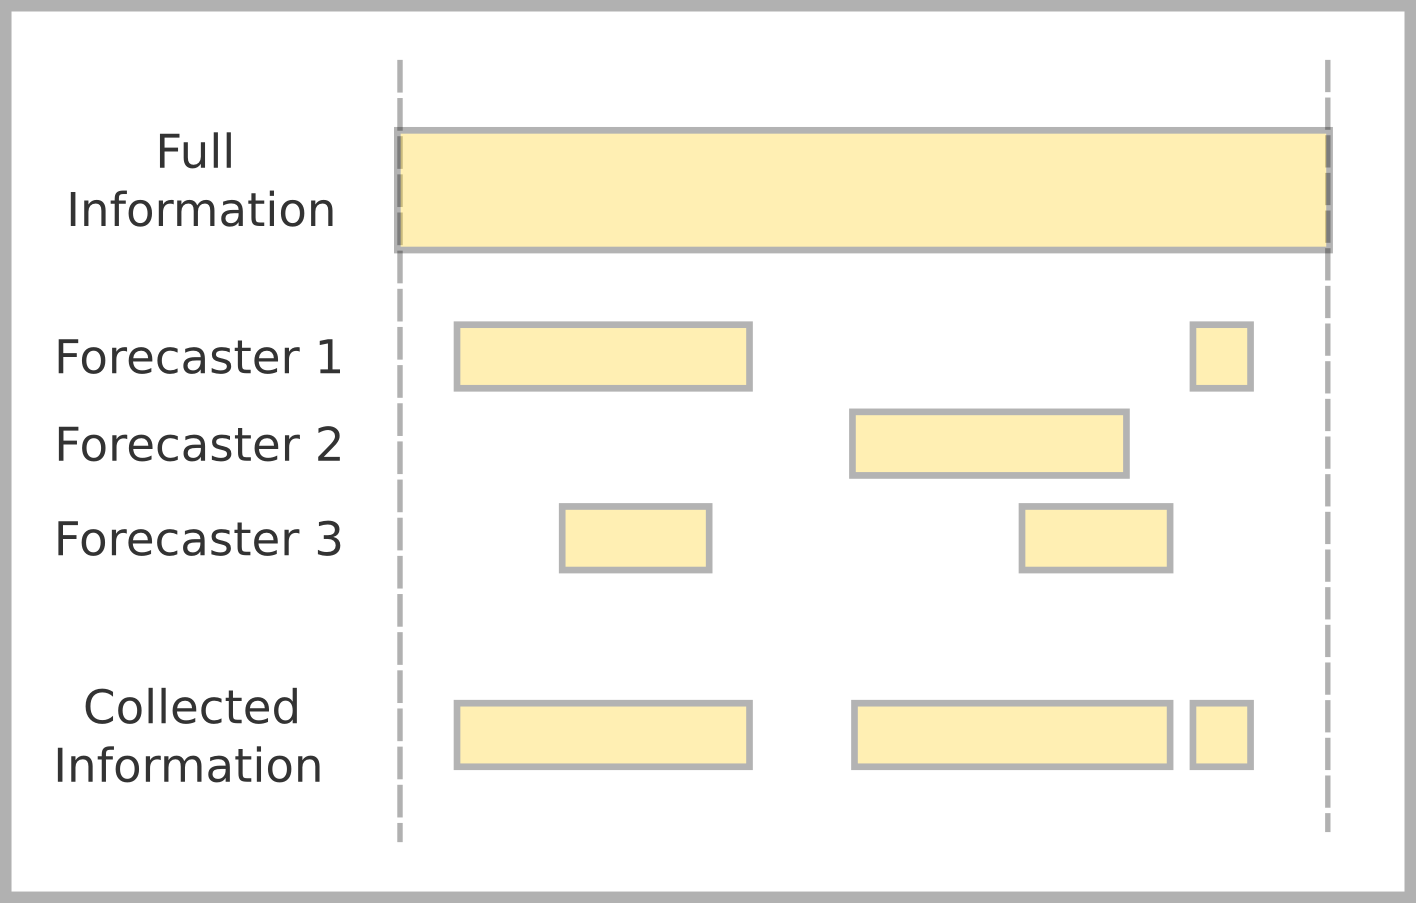
\includegraphics[width = 0.5\textwidth]{N=N.png} % requires the graphicx package
   \caption{Illustration of information collection under $N=3$ forecasters. The top bar represents $\F$ that contains all possible information that can be known about $Y$. Horizontally aligned with Forecaster $j$ is the partial information $\F_j$ revealed by that forecaster. The collected information $\F''$ is the union of the forecasters' partial information sets.}
   \label{CollectInfo}
\end{figure}

\begin{class}[Information Collectors]\label{infoAgg}
Consider $N$ forecasts $X_j$ of the outcome $Y$. An aggregator $\mathcal{X}''$ collects information if there exists a probability space $(\Omega, \F, \P)$ under which $\mathcal{X}'' = \E(Y | X_1, \dots, X_N)$ or, equivalently, $\mathcal{X}'' = \E(Y | \F'')$ with $\F'' = \sigma(X_1, \dots, X_N)$. 
%Sometimes $\mathcal{X}''$ is called the revealed aggregator because it uses all the information that the forecasters' reveal through their predictions. 
%Suppose the outcome $Y$ and its forecasts $X_j$, for $j = 1, \dots, N$, are defined on some probability space $(\Omega, \F, \P)$. Under this space, the \textit{revealed aggregator} is defined as the conditional expectation $\mathcal{X}'' := \E(Y | \F'') = \E(Y | X_1, \dots, X_N)$. This aggregator represents the forecasters' combined information   and hence is said to collect information. 
\end{class}
%, namely the $\sigma$-field generated by the individual forecasts. 
 %This forecast is called the \textit{revealed
%aggregator} because it uses all the information that the
%forecasters' reveal through their forecasts.  In fact, by the uniqueness of conditional expectation, it is the only aggregator that performs such information collection.
%Even though
%$\mathcal{X}'' $ is typically too abstract to be applied in practice,
%it provides an optimal baseline for aggregation
%efficiency. 
%Therefore it provides an ideal benchmark for
%understanding aggregators currently used in practice. 
Observe that each $\mathcal{X}''$ is paired with a probability space under which it collects information. 
\cite{dawid1995coherent} call such pairs \textit{compatible} and give some results on how to construct one from the other. At this point, however, our focus is not on any specific pair. Therefore $\mathcal{X}''$ is a generic aggregator that represents the entire class of information collectors. If some aggregator does not satisfy the condition in Definition \ref{infoAgg}, it does not collect information. Furthermore, it is deemed \textit{inefficient} because it does not use the forecasters' combined information under any probability space.
% under which it would use all the forecasters' information. 
%In this paper an aggregator is said to collect information if and only if it is a member of class described by Definition \ref{infoAgg}. 
In order to understand the behavior of these information collectors, the next theorem enumerates some of their properties. 
% At this level $\mathcal{X}''$ is very abstract and clearly cannot be applied in practice. Fortunately, however, its properties can be studied. 
%  These are summarized in the following theorem. 
  The proofs of this and all other theorems are deferred to the Appendix.

%\marginpar{What do we mean by "collect information" and does not collect information. Need a picture. Brain analogy}

%WRITE OUT A CLASS OF AGGREGATORS HERE AND EXPLAIN THAT IT DEPENDS ON THE PROBABLITY SPACE. THAT IS, A SPECIFIC INSTANCE OF X'' COLLECTS INFORMATION UNDER A CERTAIN PROBALITY SPACE. 
%\marginpar{Explain that X'' really coincides with the maximizing sharpness subject to calibration. It is the limit. }

%\marginpar{If one has a model, why cannot one just directly compute the $X''$ by taking the expectation. This leads to the curse of dimensionality. }

%COLLECTS INFOMRATION IF AND ONLYF IF IT IS EQUAL TO X'' FOR SOME PROBABLITY MODEL. 

\begin{theorem} \label{optimal}
%Suppose that $X_j = \E(Y | X_j)$ for all $j = 1, \dots, N$ and denote the revealed aggregator with $\mathcal{X}'' = \E(Y | \F'')$, where $\F'' = \sigma(X_1, \dots, X_N)$. 
%The individual forecasts agree with $Y$ in expectation, that is, $\E(X_j) = \E(Y) = \mu_0$. 
%Let $\delta_{max} := \max_j \{ \Var(X_j)  \}$ be the maximal variance among the individual forecast.
% $\delta_{max} = \E[(\mu_0 - X_j)^2]$. 
 An information collector $\mathcal{X}''$ has the following properties. 
\begin{enumerate}[i)] \label{properties}
%\item  $\mathcal{X}''$ is invariant to invertible transformations of the forecasts: if $f(\cdot)$ is an invertible transformation, then $\mathcal{X}'' = \E(Y|X_1, \dots, X_N) = \E(Y | f(X_1), \dots, f(X_N))$. 
\item $\mathcal{X}''$ is \textit{marginally consistent}:  $\E(\mathcal{X}'') = \E(Y) :=  \mu_0$.
\item $\mathcal{X}''$ is \textit{calibrated}: $\E(Y|\mathcal{X}'') = \mathcal{X}''$. 
\item $\mathcal{X}''$ is \textit{expanding}: $\max_j \{ \Var(X_j)  \} \leq \Var(\mathcal{X}'')$. 
%In words, the variance of $\mathcal{X}''$ is always at least as large as that of the most variable forecast. 
%\item \textbf{Information Collection.} $\mathcal{X}''$  is the only aggregator that uses all the information contained in the forecasts $X_1, \dots, X_N$. In other words, $\mathcal{X}''$ is the only aggregator that collects information. 
\item If $\E\left(Y^2\right) < \infty$, 
% the conditional expectation
%$\mathcal{X}'' := \E(Y | \F'')$ 
$\mathcal{X}''$ is the aggregator that minimizes the expected value of a large class of loss functions, including the quadratic loss \citep{satopaamodeling2}. 
\end{enumerate}
\end{theorem}
%Marginal consistency states that the forecast and the outcome agree in expectation.
According to item ii), $\mathcal{X}''$ is calibrated. This property is rather obvious after discussing Proposition \ref{calibrationProp} because, by definition, $\mathcal{X}''$ is based on $\F''$. 
% or, equivalently, based on some information set about $Y$. 
% Intuitively, this should be expected from an information collector. 
 Item i) shows that $\mathcal{X}''$ is also marginally consistent. In fact, if a forecast $X$ is calibrated, then $\E(X) = \E[\E(Y|X)] = \E(Y) = \mu_0$. Consequently, all calibrated forecasts (individual or aggregate) are marginally consistent. The converse, however, is not true. For instance, Theorem \ref{contraction} shows that any non-trivial weighted average is marginally consistent but not calibrated. This is an important observation that provides a technique for proving lack of calibration via marginal inconsistency -- a task that is generally much easier than disproving calibration directly. In fact, the proof of Theorem \ref{contractionXphi} makes use of this shortcut. 

%\marginpar{Theorem: $X''$ is the only aggregator that collects information.}
%\marginpar{Explain how to calibrate forecasts based on $\P$.}

To interpret the rest of the theorem, consider
%Proposition \ref{calibrationProp} combined with the fact that conditional expectation contracts in $L^2$ \citep[Theorem 5.1.4.]{durrett2010probability} show that the variance of any calibrated forecast (individual or aggregate) is upper-bounded by $\Var(Y)$. 
%%This follows directly from the fact that each reliable forecast can be associated with a sub-$\sigma$-field and the fact that conditional expectation is a contraction in $L^2$ \citep[Theorem 5.1.4.]{durrett2010probability}. 
%Theorem \ref{optimal} then shows that the corresponding lower bound for $\Var(\mathcal{X}'')$ is the maximum variance among the forecasters. More generally, consider 
%the least informative sub-$\sigma$-field, namely the trivial $\sigma$-field $\F_0 := \{\emptyset, \Omega\}$. A forecast based on $\F_0$ is always equal to the marginal mean $\mu_0$ and hence has zero variance. On the other hand, a forecast based on all the information, namely the principal $\sigma$-field $\F$, is equal to $Y$ and hence has variance $\Var(Y)$. 
%The intermediate cases can be understood by considering 
an increasing sequence of $\sigma$-fields $\F_0 = \{\emptyset, \Omega\} \subseteq \F_1 \subseteq \dots \subseteq \F_R \subseteq \F$ and the corresponding forecasts $X_r = \E(Y|\F_r)$ for $r = 0,1, \dots, R$. \citet[Proposition 2.1]{satopaamodeling2} shows that the variances of these forecasts respect the same order as their information sets; that is, $\Var(X_0) \leq \Var(X_1) \leq \dots \leq \Var(X_R) \leq \Var(Y)$, which suggest that the amount of information in a calibrated forecast is measured by its variance. Naturally, if an aggregator collects information from a group of calibrated forecasters, it should use at least as much information as the most informed individual among them. Therefore an information collector is necessarily at least as variable as each of the individual forecasts. This is precisely what item iii) describes. The final item iv) shows that $\mathcal{X}''$ is the optimal aggregator under different loss functions and hence justifies information collection as a reasonable goal in forecasts aggregation.
%This is a necessary condition for an aggregator to be a collector of information.
% Therefore any aggregator that \textit{expands} variance and satisfies this condition is
%%because it is expected to deviate more from the marginal mean than any of the individual forecasts. This is a necessary condition for an aggregator to be 
%considered a collector of information. 

%\marginpar{Do we want to discuss the coherence idea somewhere}

%If variance represents the amount of information, then a reasonable goal in aggregation is to maximize variance subject to calibration. Previously this goal has been well-established in the probability forecasting literature \citep{murphy1987general, gneiting2007probabilistic}. There a calibrated and highly variable forecast  is
%very useful to the policy-maker because it is both accurate and close
%to the most confident values of zero and one. Of course, no aggregator can use more information than $\F''$. Therefore a calibrated aggregator cannot be more variable than $\mathcal{X}''$. As a result, the general goal of maximizing variance subject to calibration is equivalent to aiming to be as close to $\mathcal{X}''$ as possible. Item iv) recasts this goal in terms of minimizing a class of loss functions. 

%Overall, this discussion poses an interesting hypothesis: 
%does Definition \ref{infoAgg} contain any measure of central tendency? 
In practice, the most common way of aggregating forecasts is with some measure of central tendency. These by definition aim to summarize the forecasts with a single central value. Given that, in expectation, this is likely to be closer to $\mu_0$ than the most variable forecast, these aggregators end up having a too low variance and hence not collecting information. To illustrate, suppose all forecasters independently predict a probability of $0.9$ for some future event. If these forecasters are using different information, then clearly their combined information should lead to an aggregate somewhat greater than $0.9$. In this simple scenario, however, all measures of central tendency aggregate to $0.9$. They do not account for the information heterogeneity among the forecasters and hence cannot collect their information. 
%In fact, \cite{satopaamodeling} explain that averaging-like techniques work well when the individual forecasters have very similar sets of information, that is, when there really is no information aggregation problem to begin with.
Instead, they reduce ``measurement error,'' which is philosophically very different to the idea of information aggregation discussed in this paper. This intuition is explored more carefully and rigorously in the following sections. 

% Past literature has acknowledged this but has typically worded it as maximizing sharpness subject to calibration. Here sharpness measures how far the forecasts are from the naive baseline forecast $\mu_0$. 
%
%They
% explain how the quality of a probability forecast
%(individual or aggregate) is typically measured in terms of
%\textit{reliability} and \textit{resolution} (sometimes also known as calibration and
%sharpness, respectively). Reliability describes how closely the
%conditional event frequencies align with the forecast
%probabilities. Resolution, on the other hand, measures how far the
%forecasts are from the naive baseline forecast, that is, the marginal
%event frequency. A forecast that is reliable and highly resolute is
%very useful to the policy-maker because it is both accurate and close
%to the most confident values of zero and one. Therefore a
%well-established goal in probability forecasting is to maximize resolution subject to
%reliability \citep{murphy1987general, gneiting2007probabilistic}.
%
%
%Recall that in probability forecasting a well-established goal is to maximize resolution subject to reliability. This goal can be easily interpreted intuitively with the help of partial information. First, conditioning on reliability requires the forecast to be consistent with some set of information about $Y$. Maximizing the resolution of this forecast takes it as far from $\mu_0$ as possible. This is equivalent to increasing the variance of the forecast as close to the theoretical upper bound $\Var(Y)$ as possible. Therefore the goal is equivalent to maximizing the amount of information that the forecast is consistent with. Intuitively, this is very reasonable and should be considered as the general goal in forecasting.


%\subsection{Weight Functions}
%This section explores what we really know about the weight functions. These functions input the predictions $X_1, \dots, X_N$. However, given that each of these forecasts is a function of $Y$, the weights can be also considered to be functions of $Y$ and the forecasters' information sets. This can be a bit confusing however because the weight function does not apply the information set in anything but the conditional expectation. Hence it may be clearer to just think about these weight functions as functions of the predictions. 
%\begin{enumerate}
%\item If $\E \sum_j w_j X_j = \mu_0$, then $\sum_j \Cov(w_j,X_j) = 0$. 
%\item $\sum_j w_j = 1$
%\item 
%\end{enumerate}

%\marginpar{We must explain somewhere why we care about the random weighted average; show with examples that this includes many of the averages such as the geometric mean, etc.  This captues the General Mean function for a finite t; see Steele's book}
%
%
%"The challenge is to identify ways to extract the maximum amount of predictive informa- tion form judgment and to us this information effectively to improve forecast accuracy" Nada Sanders and Larry Ritzman in Judgmental Adjustments of Statistical Forecasts. 







\section{WEIGHTED AVERAGING} \label{contractionSection}

%EPLAIN HERE THAT AVERAGING THE NONCALIBRATED IS NOT THE SAME AS AVERAGING THE CALIBRATED. HOWEVER, BUDESCU SHOW THAT CALIBRATING FIRST AND THEN AVERAGING INCREASES PERFORMANCE. 
%
%``An equal-weights rule offers a
%reasonable starting point, and a trimmed mean is desirable if you combine forecasts resulting
%from five or more methods. Use different weights if you have good domain knowledge or
%information on which method should be most accurate." Armstrong
%
%weights can be determined by Newbold and Granger 1974
%
%
%WRITE AS BOLD AGGREGATOR CLASS 1: EXPLAIN WHAT WEIGHTED AVERAGE IS. 

This section continues the analysis by \cite{dawid1995coherent} and \cite{Ranjan08} of the most commonly used aggregator, namely the weighted average. More precisely, the focus is on the following class of aggregators.
\begin{class}[Weighted Averages] \label{Xw}
The weighted average is $\mathcal{X}_w := \sum_{j=1}^N w_jX_j$, where each weight $w_j \geq 0$ is fixed and $\sum_{j=1}^N w_j = 1$. 
\end{class} 
%The following theorem shows that a non-trivial weighted average is neither expanding nor calibrated. Therefore it is ne can be considered suboptimal.
The most famous member of this class is the equally weighted average $\frac{1}{N}\sum_{j=1}^N X_j$ that sets all $w_j = 1/N$. Overall, the class turns out to be large yet specific enough for us to prove some detailed and useful results. These are given in the following theorem that analyzes $\mathcal{X}_w$ in the light of the properties discussed in Theorem \ref{optimal}. 
% The proof is again deferred to the Appendix. 


\begin{theorem}\label{contraction}
%Suppose that $X_j = \E(Y | X_j)$ for $j = 1, \dots, N$.  
Let $m = \argmax_j \{ \Var(X_j)  \}$ identify the forecast with the maximal variance; that is, $\Var(X_j) \leq \Var(X_m)$ for all $j = 1, \dots, N$. 
% $\delta_{max} = Var(X_m)$.  
 Then the weighted average $\mathcal{X}_w$ has the following properties. 
%Then the following holds.
\begin{enumerate}[i)]
\item  $\mathcal{X}_w$ is marginally consistent: $\E(\mathcal{X}_w) = \mu_0$. 

\item $\mathcal{X}_w$ is not calibrated, that is, $\P\left[\E(Y | \mathcal{X}_w) \neq \mathcal{X}_w\right] > 0$ if there exists a forecast pair $i \neq j$ such that $\P(X_i \neq X_j) > 0$ and $w_i, w_j > 0$. In words, $\mathcal{X}_w$ is necessarily uncalibrated if it assigns positive weight to at least two different forecasts. 
 
 \item Under the conditions of item ii), $\Var(\mathcal{X}_w)$ is too low. More specifically, if $\mathcal{X}_w' :=  \E(Y| \mathcal{X}_w)$ is the calibrated version of $\mathcal{X}_w$, then $\E(\mathcal{X}_w) = \E(\mathcal{X}_w') = \mu_0$ but $\Var(\mathcal{X}_w) < \Var(\mathcal{X}_w')$. In other words, $\mathcal{X}_w$ is under-confident in a sense that it is, in expectation, closer to the marginal mean $\mu_0$ than its calibrated version $\mathcal{X}_w'$. \label{underconfA}
 
\item $\mathcal{X}_w$ is not expanding: $\Var(\mathcal{X}_w) \leq \Var(X_m)$. This shows that $\mathcal{X}_w$ is under-confident in a sense that it is, in expectation, closer to the marginal mean $\mu_0$ than the revealed aggregator $\mathcal{X}''$.  Furthermore, $\Var(\mathcal{X}_w) = \Var(\mathcal{X}'')$ if and only if both $\mathcal{X}_w = \mathcal{X}'' = X_m$; that is,  $X_m$ contains all the forecasters' combined information, 
%provides all the information necessary for $\mathcal{X}''$, 
and $\mathcal{X}_w$ assigns all weight to $X_m$ (or to a group of forecasts equal to $X_m$). \label{underconfB}
\end{enumerate}
\end{theorem}

%NOT SURE IF IT NEEDS TO BE SAID THAT THERE MAY BE A GROUP OF FORECASTS ALL AGGREEING WITH THE MAXIMUM. EACH FORECASTER IS LIKELY TOH AVE DIFFERENT INFORMATION, AND HENCE THEIR VARIANCE MUST BE DIFFERENT. THIS IS FROM DURRET. 
%THE WEIGHTS DO NOT HAVE TO POSITIVE, THEY JUST HAVE TO SUM TO ONE. MAKE THIS GENERALIZATION. USE $\alpha$'s to make the linear weights. Be careful, expanding condition may require the weights to be positive. 
%\marginpar{Even if the weights here are allowed to be equal to one, the variance of the aggregator cannot exceed that of the forecasts. Therefore the X'' meets the weighted average only when there is an oracle forecaster and all weight has been assigned to it. Discuss this instead of the variance argument}

%Given that under-confidence is a relative concept, it requires a baseline
Items i) to iii) generalize \citet[Theorem 2.1.]{Ranjan08} from binary outcomes to any type of outcomes. 
%More specifically, the final two items 
%This theorem discusses under-confidence with respect to two different baselines. First, item \ref{underconfA}) generalizes 
% Intuitively, it states that if $\mathcal{X}_w$ is trained to use its information accurately, the resulting aggregator is more confident. 
More specifically, item iii) defines and considers under-confidence relative to the calibrated version of  $\mathcal{X}_w$. Given that $\mathcal{X}_w$ is closer to $\mu_0$ than its calibrated version, the noise or negative information in $\mathcal{X}_w$ has the effect of contracting towards $\mu_0$. 
%Under this kind of comparison, however, a calibrated aggregator is never under-confident. For instance, an aggregator that ignores the individual forecasts and always returns the marginal mean $\mu_0$ is calibrated and hence would not be considered under-confident. Intuitively, however, it is clear that no forecast is more under-confident than $\mu_0$. To avoid this problem, 
Item \ref{underconfB}), on the other hand, defines under-confidence relative to $\mathcal{X}''$. This checks whether $\mathcal{X}_w$ is as confident as it should be, given the information it received through the forecasts. Unfortunately, $\mathcal{X}_w$ is under-confident unless it assigns all the weight  to a forecaster whose information set contains every other forecasters' information. Even if $\mathcal{X}_w$ could pick out the most informed forecaster ex-ante, the chances of a single forecaster knowing everything that the rest of the forecasters know is extremely small in practice. In essentially all other cases, $\mathcal{X}_w$ is not expanding or calibrated and hence cannot equal $\mathcal{X}''$ under any probability model. This is emphasized in the following corollary.

%. Comparing this to $\mathcal{X}''$ then gives the following corollary.  
%Consequently, its variance cannot be interpreted as the amount of used information. 


\begin{corollary}
$\mathcal{X}_w$ does not collect information as long as it assigns positive weight to at least two different forecasts. 
\end{corollary}
%\marginpar{To put this in another way, there is not probability model under which Xw is the optimal aggregator.}

% but then modifies it slightly in order to derive new sub-optimality results.  
%to understand when members of this can and cannot collect information. 

% the aggregator class to be analyzed in the next section.
% to be analyzed in the next section. 
%For instance, if $f(X_1,X_2)$ is one of these measures of central tendency, 

% shortcoming spans across all measures of central tendency. These aggregators reduce variance and hence are separated from the revealed aggregator by the maximum variance among the individual forecasts. For instance, \cite{papadatos1995maximum} discuss the maximum variance of different order statistics and show that the variance of the median is upper bounded by the global variance of the individual forecasts. Given that such aggregators are not expanding, they cannot be considered to collect information. 

%This gives us motivation to analyze a broader class of aggregators. 

%For instance, under measurement error an aggregator with a relatively high variance is  considered to be less precise, whereas under partial information increased variance represents more information and hence better forecasting accuracy. 

%\marginpar{Another interesting idea is this: if all forecasters report, say, 0.9 the average is always equal to 0.9 -- not matter what the information overlap is. it is however reasonable to think that if more and more people give the estimate 0.9, the the combined evidence should give something much closer to 1. This is why they are not information collectors; this is probably best in the introduction. Also, this is bvery clear because it is prob forecasts. We however make it specific for all univariate forecasts and show that no matter what they are, averaging is not collection info.}
%
%\marginpar{information diversity pushes outwards while measurement error pulls inwards. Opposing forces.}
%\marginpar{make sure mention averaging not info collecting in the intro}

%This stands in sharp contrast with what increased variance represents under partial information. 

%Theorem \ref{contraction}, however, is not only negative in nature; it is also  constructive in several different ways. First, 
%%given that averaging aggregators are under-confident, a simple adjustment is to  increase their variance by transforming them systematically away from the marginal mean $\mu_0$. 
%%This
%it motivates a general and precise definition of extremizing:
%\begin{definition} \label{extrem}
%\textbf{Extremization.}
%Consider two reliable forecasts $X_i$ and $X_j$. Denote their common marginal mean with $\E(X_i) = \E(X_j) = \mu_0$. The forecast $X_j$ \textit{extremizes} $X_i$ if and only if either $X_j \leq X_i \leq \mu_0$ or $\mu_0 \leq X_i \leq X_j $ always holds.
%\end{definition}
%
%\noindent
%It is interesting to contrast this definition with the popular extremization heuristic in the context of probability forecasting.  Definition \ref{extrem} suggests that simply moving, say, the average probability forecast closer to zero or one improves the aggregate if and only if the marginal probability of success is $0.5$. In other cases naively following the heuristic may end up degrading the aggregate. For instance, consider a geographical region where rain is known to occur on $20$\% of the days. If the average probability forecast of rain tomorrow is $0.30$, instead of following the heuristic and shifting this aggregate towards zero and hence closer to the marginal mean of $0.20$, the aggregate should be actually shifted in the opposite direction, namely closer to one. Second, Theorem \ref{contraction} suggests that extremization, as defined formally above, is likely to improve the weighted average of any type of univariate forecasts. This justifies the construction of a broader class of extremizing techniques. In particular, the second part of item \ref{underconfB}) states that extremizing is likely to improve the weighted average when 
%%not required when the weighted average is able to give full weight to a single forecaster who happens to know everything that the other forecasters know. In all other cases and in particular when
% the single most informed forecaster knows a lot less than all the forecasters know as a group. To illustrate this, the next section introduces a simple optimization procedure that extremizes the weighted average of real-valued forecasts.
%% and applies it to two examples involving both synthetic and real-world data.
%%
%% This is precisely what extremizing does. Therefore it is not surprising that extremizing has been observed to improve the predictive accuracy of many simple aggregators of  probability forecasts. 
%%%To the best of our knowledge, however,  no previous study has illustrated the benefits of extremizing real-valued forecasts. 
%%This is the main topic in the rest of the paper.
%%
%%The next section introduces a simple optimization procedure that extremizes the weighted average of real-valued forecasts. 
A similar inefficiency result does not hold for all linear combinations (with an intercept term) of the forecasts. For instance, \cite{dawid1995coherent} describe a Binomial model under which $\mathcal{X}''$ is a linear combination of the individual $X_j$'s. Such techniques, however, are outside the scope of this paper. As was mentioned before, the focus here is on averaging-like techniques and other measures of central tendency. 
%Theorem \ref{contraction} gives a rather thorough analysis of the weighted average. 
This section analyzed direct averaging of the forecasts. Sometimes in practice, however, the forecasts are transformed before averaging. For instance, if the forecasts are expressed as ratios to a reference value, then the decision maker may want to use a geometric mean instead of an arithmetic mean. This and other similar aggregators are analyzed in the next section.
%The next section analysis the inefficiency of such aggregators. 


\section{TRANSFORMED WEIGHTED AVERAGING} \label{TranscontractionSection}
%\url{https://books.google.co.uk/books?id=2KC9uigO_04C&pg=PA370&lpg=PA370&dq=monotone+transformation+variance&source=bl&ots=oomq3d87xT&sig=dR3ZwqOe-zebI4VgZkOHbFWE1ig&hl=en&sa=X&ved=0ahUKEwi57sDjhf3PAhVmD8AKHeN9CK4Q6AEISzAH#v=onepage&q=monotone%20transformation%20variance&f=false}
%Ordinarily transform non-negative data. Monotonicity maintains information and does not transform two different values to the same value. 

This section expands Definition \ref{Xw} to allow transformations of the forecasts. In particular, the analysis focuses on the following class of aggregators.
\begin{class}[Transformed Weighted Averages] \label{Xphi}
Consider some strictly monotone function $\Phi: \supp(X_j) \to S \subseteq \R$. The transformed weighted average associated with $\Phi$ is then $\mathcal{X}_{\Phi} := \Phi^{-1} \left( \sum_{j=1}^N w_j \Phi(X_j) \right)$, where each weight $w_j \geq 0$ is fixed and $\sum_{j=1}^N w_j = 1$. 
\end{class} 
In other words, the idea is to transform the calibrated forecasts $X_j$ to some other space, average the transformed forecasts, and then transform the average back to the original space. The function $\Phi$ is required to be strictly monotonic so that its inverse exists. This also maintains order and ensures that two different forecasts are not mapped to the same value. From an information perspective, a strictly monotonic function preserves information; that is, $\sigma(X_j) = \sigma(\Phi(X_j))$. Clearly, if $\mathcal{X}_\Phi$ is to collect information from the original forecasts $X_j$, the transformation $\Phi(X_j)$ cannot lose any of the original information content. Thus, monotonicity is essential.  Despite this requirement, however, the following theorem states that $\mathcal{X}_\Phi$ often does not collect information. 
%This is made more precise in the following theorem.
%Some well-known members of this class are discussed shortly. First, however, the next theorem describes subsets of the class that never collect information. 
%In a forecasting application, the function $\Phi$ is typically strictly increasing and hence maintains the order among the forecasts. In contrast, a strictly decreasing function would reverse the order of the forecasts. Intuitively this hardly makes sense; it is as if the forecasters had been predicting $-Y$ instead of $Y$. Nonetheless, 

\begin{theorem}\label{contractionXphi}
%Suppose that 
%The following considers two subsets of the transformed weighted averages, characterized by the type of $\Phi$ and $\supp(X_j)$, namely the support of the forecasts: 
Suppose that $\mathcal{X}_\Phi$ assigns positive weight to at least two different forecasts. Then it has the following properties. 
\begin{enumerate}[i)]
\item If $\Phi$ is convex or concave, then $\mathcal{X}_\Phi$ is not calibrated and hence does not collect information. Furthermore, if $\Phi$ is strictly convex or concave, then  $\mathcal{X}_\Phi$ is not even marginally consistent. 
\item If $\Phi: \supp(X_j) \to S \subseteq \R^+$ is continuous and $X_j \geq 0$, then $\mathcal{X}_\Phi$ does not collect information. 
\end{enumerate}
\end{theorem}
The items of this theorem complement each other
%: one places no constraints on $\supp(X_j)$ but considers a smaller collection of $\Phi$'s. Together they
and capture 
%This Theorem \ref{contractionXphi}
many well-known aggregators. For instance, the results apply to the entire class of \textit{weighted generalized means} 
\begin{align*}
\mathcal{X}_a := \left( \sum_{j=1}^N w_j X_j^a \right)^{1/a},
\end{align*}
where $X_j \geq 0$ and $a \in \R$ is a given constant. Here the function $\Phi(x) = x^{a}$ is concave if $a \in [0,1]$ but convex otherwise. Notable members of this class include the harmonic, geometric, arithmetic, quadratic, and cubic means, corresponding respectively to $a = -1, 0, 1, 2, 3$. Thus, by Theorem  \ref{contractionXphi}, none of these aggregators collect information. In fact, they are not even calibrated and hence based on any information set about $Y$.

%The inefficiency of the generalized means follows from either item of Theorem  \ref{contractionXphi}. While the first item does not restrict $\supp(X_j)$ in any way, the second item restricts $X_j$ and $\Phi(X_j)$ to either half of the real-line such that $\sign(X_j \Phi(X_j))$ is fixed. In practice the forecasts are typically non-negative. If these forecasts are not calibrated, a common approach is to transform them by a monotonic function within their own space before aggregation. This and its connection to Theorem \ref{contractionXphi} is discussed in more detail in Section \ref{nonExperts}. 

%\marginpar{ the aggregator does not collect information as long as it assigns positive weight to at least two different forecasts. }

%Even though Theorem \ref{contractionXphi} is more general than Theorem \ref{contraction}, the
Unfortunately, the results discussed so far do not apply to many commonly used measures of central tendency, such as the median, midrange, or trimmed averages.  In short, this is because such aggregators do not treat the forecasts symmetrically ex-ante but instead depend on the realized values of the forecasts. 
%the weights would have to change as function of the forecasts. 
%Aggregation Class \ref{Xw}, however, considers the weights as fixed. 
The key towards a fully general analysis is to observe that all measures of central tendency are constrained to the convex hull of the forecasts. This property defines a new aggregator class that is analyzed in the next section.
%contains all measures of central tendency. The next section analyzes this class.



\section{MEASURES OF CENTRAL TENDENCY}\label{RandomSection}

%This is a very general class of aggregators. Therefore it is more difficult to make as detailed claims as in Theorem . For instance, the class is contains aggregators that are marginally consistent but not expanding (e.g., all of Class \ref{Xw}), and conversely aggregators that are expanding but not marginally consistent (e.g., $\min(X_j)$ or $\max(X_j)$). The goal, however, is to understand when aggregators in this class can and cannot collect information from the forecasters; that is, under what conditions $\mathcal{X}''$ is in this class. 

\subsection{Random Convex Combinations}
This section analyses aggregators that remain within the convex hull of the individual forecasts. 
These aggregators, called random convex combinations, are defined as follows. 

\begin{class}[Random Convex Combinations] \label{Xc}
The random convex combination $\mathcal{X}_{[\cdot]}$ is always within the convex hull of the forecasts, that is, $\mathcal{X}_{[\cdot]} \in [\min(X_j), \max(X_j)]$. The subindex here reminds that $\mathcal{X}_{[\cdot]}$ can take on any value within the closed convex hull. 
\end{class} 
%More specifically, if $\mathcal{X}$ denotes the aggregator, then 
%\begin{align}
%\mathcal{X}(\omega) \in [\min(X_j)(\omega), \max(X_j)(\omega)] \label{convexity}
%\end{align}
% for all $\omega \in \Omega$. 
% The goal is to understand when such an aggregate can and cannot collect information from the forecasters. This is a very general class of aggregators and includes all commonly used measures of central tendency such as the median, generalized average (with geometric mean, harmonic mean, and others), mid-range, trimmed means, and so on. 
%The plan is to first examine these aggregators in the most general probability space, and then add constraints as needed. 
%WHAT IS OUR STRATEGY HERE: TO START AS GENERAL AS POSSIBLE AND THEN MAKE AS FEW ASSUMPTIONS OR RESTRICTIONS AS POSSIBLE. 
%Write the random average as $\sum_{j=1}^N w_j X_j$, where $w_j$ is considered random. Thus $w_j$ is a function of $\omega \in \Omega$. However, for each $\omega$, they must satisfy $\sum_{j=1}^N w_j(\omega) = 1$. Hence the vector of weights can be viewed as a random point on the $N$-simplex. To begin our analysis, 
%This section shows that an aggregate satisfying (\ref{convexity}) can collect information. Thus criterion (\ref{convexity}) is too loose. 
%\marginpar{Somwhere we must be more specific about what is actually contained in this class. Should we write a separate class. }
Observe that this definition does not specify the functional form of the aggregator. The only requirement is that it remains within the convex hull under any realization of the forecasts. Therefore this is clearly the most general class of aggregators considered so far in this paper. In particular, it contains all measures of central tendency but also the other classes defined in Definitions \ref{Xw} and \ref{Xphi}. Unfortunately, this class is slightly too large for a general inefficiency result. This is illustrated in the following example. 
%Fortunately, the class can be modified slightly without excluding any measures of central tendency. 
\begin{example}\label{Example1}
Consider rolling a fair die and predicting whether the result is an even number. This can be described with the following probability model. Suppose $\Omega = \{\omega_1, \dots, \omega_6\}$ and let $\F = 2^\Omega$ be all subsets of $\Omega$. The outcome is $Y(\omega) = \one_A(\omega)$, where $A = \{\omega_2, \omega_4, \omega_6\}$, and $\P$ is uniform over $\Omega$; that is, $\P(A) = |A|/6$ for all $A \in \F$.  Consider two forecasters with the following information sets: $\F_1 = \sigma(\{\omega_1\})$ and $\F_2 = \sigma(\{\omega_6\})$. Their combined information is   $\F'' = \sigma(\F_1, \F_2) =  \sigma(\{\omega_1\}, \{\omega_6\})$. These three information sets are illustrated in Figure \ref{ExamplePartitionFinite}. The relevant forecasts are
\begin{align*}
X_1(\omega) &= \begin{cases}
0 & \text{ if } \omega = \omega_1\\
3/5& \text{ otherwise} 
\end{cases},&
X_2(\omega) &= \begin{cases}
1 & \text{ if } \omega = \omega_6\\
2/5 & \text{ otherwise} 
\end{cases},  &
\mathcal{X}'' &= \begin{cases}
0  & \text{ if } X_1 = 0 \\
1  & \text{ if } X_2 = 1\\
1/2 & \text{ otherwise} 
%1/2 = ( X_1(\omega) + X_2(\omega))/2 & \text{ otherwise} 
\end{cases}.
\end{align*}
%Each forecast here is calibrated. Their shared mean is $\E(Y) = 1/2$. The variances are $\Var(Y) = 1/4$, $\Var(X_1) = \Var(X_2) = 1/20$, and $\Var(X'') = 1/12$. Note that these are all in the order explained by the theory.
% \marginpar{This all could be recast as rolling a die. }
\end{example}
This example constructs an outcome and a probability space under which the information collector $\mathcal{X}''$ is a random convex combination. This means that $\mathcal{X}_{[\cdot]}$ can collect information. More specifically, however, the example was chosen to illustrate that $\mathcal{X}_{[\cdot]}$ can do this if it is allowed to equal  the minimum or maximum forecast when some of the forecasts disagree. Fortunately, if Definition \ref{Xc} is tightened slightly such that this is not allowed, the class still contains essentially all measures of central tendency but general inefficiency results can be proven. This is the topic in the next subsections.
% The next subsection analyzes these aggregators under two different levels of forecaster information. 

%\subsection{Random Weighted Averaging: Preliminary Example, Contiguous Information Sets}
%Consider $\Omega = \{w_1, w_2, w_3, w_4\}$. Let $\F_1 = \sigma(\{w_1,w_2\})$ and $\F_2 = \sigma(\{w_2,w_3\})$. Then $\F'' = \F$, $X'' = Y$, 
%\begin{align*}
%\E[Y|\F_1](w) &= \begin{cases}
%\frac{\P(w_1)Y(w_1) + \P(w_2)Y(w_2)}{\P(w_1) + \P(w_2)} & w \in \{w_1, w_2\}\\
%\frac{\P(w_3)Y(w_3) + \P(w_4)Y(w_4)}{\P(w_3) + \P(w_4)} & w \in \{w_3, w_4\}
%\end{cases}
%\end{align*}
%and
%\begin{align*}
%\E[Y|\F_2](w) &= \begin{cases}
%\frac{\P(w_2)Y(w_2) + \P(w_3)Y(w_3)}{\P(w_2) + \P(w_3)} & w \in \{w_2, w_3\}\\
%\frac{\P(w_1)Y(w_1) + \P(w_4)Y(w_4)}{\P(w_1) + \P(w_4)} & w \in \{w_1, w_4\}
%\end{cases}
%\end{align*}
%Denote $p_{ij} = \P(w_i) / (\P(w_i) + \P(w_j))$. Without loss of generality (one has to be larger), assume that
%\begin{align*}
%%\frac{\P(w_1)Y(w_1) + \P(w_2)Y(w_2)}{p_{12}} < Y(w_1) < \frac{\P(w_1)Y(w_1) + \P(w_4)Y(w_4)}{\P(w_1) + \P(w_4)}\\
%X_1(w_1) &< X''(w_1) < X_2(w_1)\\
%p_{12}Y(w_1) + (1-p_{12}) Y(w_2) &< Y(w_1) < p_{14}Y(w_1) + (1-p_{14})Y(w_4)
%%(1-p_{12}) Y(w_2) < (1 - p_{12} - p_{14})Y(w_1)  < (1-p_{14})Y(w_4)\\
%\end{align*}
%Here the strict inequality must hold because $w \in (0,1)$. That is, $X'' = wX_1 + (1-w)X_2$ for some random $w \in (0,1)$.  Notice that the left hand side is a weighted average of $Y(w_1)$ and $Y(w_2)$; hence is between  $Y(w_1)$ and $Y(w_2)$. Similarly, the right hand side is a weighted average of $Y(w_1)$ and $Y(w_4)$; hence is between $Y(w_1)$ and $Y(w_4)$. The only way $Y(w_1)$ can be stricly in the middle is if $Y(w_2) < Y(w_1) < Y(w_4)$. 
%
%A similar argument can be made for $w_2$. Without referring to our first result, this gives us that either  $Y(w_1) < Y(w_2) < Y(w_3)$ (if $X_1(w_2) < X_2(w_2)$) or  $Y(w_3) < Y(w_2) < Y(w_1)$ (if $X_2(w_2) < X_1(w_2)$). From our first result, however, we already know that $Y(w_2) < Y(w_1)$. Thus, only the second result can hold, and we have that  $Y(w_3) < Y(w_2) < Y(w_1) < Y(w_4)$.
%
%The argument for $w_3$ gives that either  $Y(w_4) < Y(w_3) < Y(w_2)$ (if $X_1(w_3) < X_2(w_3)$) or  $Y(w_2) < Y(w_3) < Y(w_4)$ (if $X_2(w_3) < X_1(w_3)$).  Given that we have already established that $Y(w_3) < Y(w_2) < Y(w_1) < Y(w_4)$, neither of these results can be true. Hence it is not possible to have $X'' = wX_1 + (1-w)X_2$ for some $w \in (0,1)$. This example illustrates the essential idea behind the conflict: it is physically not possible to allocate the measure and pick the values of $Y$ such that $X'' = wX_1 + (1-w)X_2$ for some $w \in (0,1)$. 
%
%
%
%
%\subsection{Random Weighted Averaging: Discrete Sample Space, Contiguous Information Sets}
%
%\textbf{Suppose that $X'' = wX_1 + (1-w)X_2$ for some random $w \in (0,1)$.}\\
%\\
%Consider $\Omega = \{w_1, w_2, \dots, w_W\}$. Suppose $\F_1 = \sigma(A_1, \dots, A_I)$ and $\F_2 = \sigma(B_1, \dots, B_J)$ for some partitions (filled from left to right) $\{A_1, \dots, A_I\}$ and $\{B_1, \dots, B_J\}$ of $\Omega$. (To justify the use of a partition: \url{http://math.stackexchange.com/questions/1441596/show-the-sigma-algebra-of-a-countable-set-is-generated-by-a-partition}) Then, $\F'' = \sigma(\{C_{ij} := A_i \cap B_j\}) = \sigma(C_1, \dots, C_K)$ (also ordered from left to right). Note that all of these partitions must satisfy the law of total expectation: $\E[Y] = \sum_i^I \E[Y | A_i] \P(A_i)$. This shows the overall budget. 
%%We can merge each $w \in C_{ij}$ into a single $w$ with the combined measured because none of the observables change if one moves from one $w$ to another within the same $C_{ij}$. Therefore we can assume that each $C_{ij}$ holds only one $w$. 
%
%\begin{align*}
%\frac{\sum_{w \in A_i} \P(w) Y(w)}{\sum_{w \in A_i} \P(w)} &= \frac{\sum_{k : C_k \cap A_i \neq \emptyset}\sum_{w \in C_k} \P(w) Y(w)}{\sum_{w \in A_i} \P(w)}\\
% &= \frac{\sum_{k : C_k \cap A_i \neq \emptyset}X''(C_k) \sum_{w \in C_k} \P(w) }{\sum_{w \in A_i} \P(w)}\\
% &= \sum_{k : C_k \cap A_i \neq \emptyset}p_{ik}X''(C_k),
%\end{align*}
%where $p_{ik} = \sum_{w \in C_k} \P(w)  / \sum_{w \in A_i} \P(w)$ and $\sum_{k : C_k \cap A_i \neq \emptyset}p_{ik} = 1$. Similarly define $q_{jk} = \sum_{w \in C_k} \P(w)  / \sum_{w \in B_j} \P(w)$. Thus both $X_1$ and $X_2$ can be written as a convex combination of $X''$ (note: this is all true for any $N$). It is not possible to have $C_k = A_i$ or $C_k = B_j$ for any $i,j,k$. If this were true, then $X''$ would match with $X_1$ or $X_2$, suggesting a weight $w = 1$ or $0$. Equality would lead to a $X''$ that is not well-defined. More specifically, this would allow any weight $w \in [0,1]$. For the sake of the argument, such equal pairs can be removed from the proof. This essentially just cuts off a piece of $\Omega$. The argument then will show that if $X_1 \neq X_2$ at least for some $\omega \in \Omega$. Therefore for now assume that no $A_i \subset B_j$ or $B_j \subset A_i$. This then means that each $A_i = C_k \cap C_{k+1}$ or $C_k \cap C_{k-1}$. Note that such a set cannot be split into more than two $C_k$'s because otherwise one of them would have to be in the middle. This middle set then would have have been formed by some $B_j$. Such a $B_j$ would be then a proper subset of $A_i$, leading again to a weight of $1$.
%% and hence would contradict our assumption.
%
%\marginpar{This assumes that sets are contigious; how to generalize from this}
%
%Now, without loss of generality (one has to be larger), assume that
%%\scriptsize
%\begin{align*}
%X_1(C_1) &< X''(C_1) < X_2(C_1)\\
% \sum_{k : C_k \cap A_1 \neq \emptyset}p_{1k}X''(C_k) &< X''(C_1)  <  \sum_{k : C_k \cap B_1 \neq \emptyset}q_{1k}X''(C_k) 
%%\frac{\sum_{w \in  A_1 / C_{11}} \P(w) Y(w) + \sum_{w \in C_{11}} \P(w) Y(w)}{\sum_{w \in A_1} \P(w)} &< \frac{\sum_{w \in C_{11}} \P(w) Y(w)}{\sum_{w \in C_{11}} \P(w)}  < \frac{\sum_{w \in B_1 / C_{11}} \P(w) Y(w) + \sum_{w \in C_{11}} \P(w) Y(w)}{\sum_{w \in B_1} \P(w)}\\
%%\frac{\sum_{w \in  A_1 / C_{11}} \P(w) Y(w) + X''(w_1)  \sum_{w \in C_{11}} \P(w) }{\sum_{w \in A_1} \P(w)} &< X''(w_1)   < \frac{\sum_{w \in B_1 / C_{11}} \P(w) Y(w) + X''(w_1)  \sum_{w \in C_{11}} \P(w) }{\sum_{w \in B_1} \P(w)}\\
%%\frac{\sum_{w \in  A_1 / C_{11}} \P(w) Y(w) +   \sum_{w \in C_{11}} \P(w) X''(w_1) }{\sum_{w \in A_1} \P(w)} &< X''(w_1)   < \frac{\sum_{w \in B_1 / C_{11}} \P(w) Y(w) +   \sum_{w \in C_{11}} \P(w) X''(w_1)}{\sum_{w \in B_1} \P(w) }
%\end{align*}
%%\normalsize
%This tells us that $\min\{X''(C_k) : C_k \cap A_1 \neq \emptyset\} < X''(C_1) < \max\{X''(C_k) : C_k \cap B_1 \neq \emptyset\}$. Now if the sets are contiguous, then (again it does not matter how we label)
%\begin{align*}
%p_{11}X''(C_1) + p_{1K}X''(C_{K}) &< X''(C_1)  <  q_{11}X''(C_1)  + q_{12}X''(C_{2}),
%\end{align*}
%which then gives that $X''(C_K) < X''(C_1) < X''(C_2)$. Now repeat this argument for $C_2$ to get that $X''(C_3) < X''(C_2) < X''(C_1)$ (if $X_1(C_2) < X_2(C_2)$)  or $X''(C_1) < X''(C_2) < X''(C_3)$ (if $X_1(C_2) > X_2(C_2)$). Of course, based on what we know from before, only the second case is possible. Hence we have established that $X''(X_K) < X''(C_1) < X''(C_2) < X''(C_3)$. You repeat this argument until the very last set. This then gives you $X''(C_{K-1}) < X''(C_K)$. A contradiction. 



%
%\subsection{Random Weighted Averaging: More Involved Example}
%Consider $\Omega = \{\omega_1, \dots, \omega_9\}$. Let $\F_1 = \sigma(\{\omega_1, \omega_2, \omega_3\}, \{\omega_4, \omega_5, \omega_6\}, \{\omega_7, \omega_8, \omega_9\})$ and $\F_2 = \sigma(\{\omega_1, \omega_4, \omega_7\}, \{\omega_2, \omega_5, \omega_8\}, \{\omega_3, \omega_6, \omega_9\})$. Then $\F'' = \F$ and $X'' = Y$. This is the smallest case that leads to each $X_i$ being a weighted average of three terms; hence it is the simplest case that represents the general complexity of the problem. If $\P(w_j) = p_j$, then
% \begin{align*} 
%\begin{cases}
%\min \{ Y(\omega_2), Y(\omega_3)\} < Y(\omega_1) < \max \{ Y(\omega_4), Y(\omega_7)\} & \text{ if } X_1(\omega_1) < X_2(\omega_1)\\
%\min \{ Y(\omega_4), Y(\omega_7)\} < Y(\omega_1) < \max \{ Y(\omega_2), Y(\omega_3)\} & \text{ if } X_1(\omega_1) > X_2(\omega_1)
%\end{cases}\\
%\begin{cases}
%\min \{ Y(\omega_1), Y(\omega_3)\} < Y(\omega_2) < \max \{ Y(\omega_5), Y(\omega_8)\} & \text{ if } X_1(\omega_2) < X_2(\omega_2)\\
%\min \{ Y(\omega_5), Y(\omega_8)\} < Y(\omega_2) < \max \{ Y(\omega_1), Y(\omega_3)\} & \text{ if } X_1(\omega_2) > X_2(\omega_2)
%\end{cases}\\
%\begin{cases}
%\min \{ Y(\omega_1), Y(\omega_2)\} < Y(\omega_3) < \max \{ Y(\omega_6), Y(\omega_9)\} & \text{ if } X_1(\omega_3) < X_2(\omega_3)\\
%\min \{ Y(\omega_6), Y(\omega_9)\} < Y(\omega_3) < \max \{ Y(\omega_1), Y(\omega_2)\} & \text{ if } X_1(\omega_3) > X_2(\omega_3)
%\end{cases}\\
%\begin{cases}
%\min \{ Y(\omega_5), Y(\omega_6)\} < Y(\omega_4) < \max \{ Y(\omega_1), Y(\omega_7)\} & \text{ if } X_1(\omega_4) < X_2(\omega_4)\\
%\min \{ Y(\omega_1), Y(\omega_7)\} < Y(\omega_4) < \max \{ Y(\omega_5), Y(\omega_6)\} & \text{ if } X_1(\omega_4) > X_2(\omega_4)
%\end{cases}\\
%\begin{cases}
%\min \{ Y(\omega_4), Y(\omega_6)\} < Y(\omega_5) < \max \{ Y(\omega_2), Y(\omega_8)\} & \text{ if } X_1(\omega_5) < X_2(\omega_5)\\
%\min \{ Y(\omega_2), Y(\omega_8)\} < Y(\omega_5) < \max \{ Y(\omega_4), Y(\omega_6)\} & \text{ if } X_1(\omega_5) > X_2(\omega_5)
%\end{cases}\\
%\begin{cases}
%\min \{ Y(\omega_4), Y(\omega_5)\} < Y(\omega_6) < \max \{ Y(\omega_3), Y(\omega_9)\} & \text{ if } X_1(\omega_6) < X_2(\omega_6)\\
%\min \{ Y(\omega_3), Y(\omega_9)\} < Y(\omega_6) < \max \{ Y(\omega_4), Y(\omega_5)\} & \text{ if } X_1(\omega_6) > X_2(\omega_6)
%\end{cases}\\
%\begin{cases}
%\min \{ Y(\omega_8), Y(\omega_9)\} < Y(\omega_7) < \max \{ Y(\omega_1), Y(\omega_4)\} & \text{ if } X_1(\omega_7) < X_2(\omega_7)\\
%\min \{ Y(\omega_1), Y(\omega_4)\} < Y(\omega_7) < \max \{ Y(\omega_8), Y(\omega_9)\} & \text{ if } X_1(\omega_7) > X_2(\omega_7)
%\end{cases}\\
%\begin{cases}
%\min \{ Y(\omega_7), Y(\omega_9)\} < Y(\omega_8) < \max \{ Y(\omega_2), Y(\omega_5)\} & \text{ if } X_1(\omega_8) < X_2(\omega_8)\\
%\min \{ Y(\omega_2), Y(\omega_5)\} < Y(\omega_8) < \max \{ Y(\omega_7), Y(\omega_9)\} & \text{ if } X_1(\omega_8) > X_2(\omega_8)
%\end{cases}\\
%\begin{cases}
%\min \{ Y(\omega_7), Y(\omega_8)\} < Y(\omega_9) < \max \{ Y(\omega_3), Y(\omega_6)\} & \text{ if } X_1(\omega_9) < X_2(\omega_9)\\
%\min \{ Y(\omega_3), Y(\omega_6)\} < Y(\omega_9) < \max \{ Y(\omega_7), Y(\omega_8)\} & \text{ if } X_1(\omega_9) > X_2(\omega_9)
%\end{cases}
%\end{align*}
%
%These can be written a bit more concisely as follows:
% \begin{align*} 
%\min \{ Y(\omega_2), Y(\omega_3), Y(\omega_4), Y(\omega_7)\} &&<&Y(\omega_1) <&& \max \{ Y(\omega_4), Y(\omega_7), Y(\omega_2), Y(\omega_3)\} \\
%\min \{ Y(\omega_1), Y(\omega_3), Y(\omega_5), Y(\omega_8)\} &&<&Y(\omega_2) <&& \max \{ Y(\omega_5), Y(\omega_8), Y(\omega_1), Y(\omega_3)\}\\
%\min \{ Y(\omega_1), Y(\omega_2), Y(\omega_6), Y(\omega_9)\} &&<&Y(\omega_3) <&& \max \{ Y(\omega_6), Y(\omega_9), Y(\omega_1), Y(\omega_2)\}\\
%\min \{ Y(\omega_5), Y(\omega_6), Y(\omega_1), Y(\omega_7)\} &&<&Y(\omega_4) <&& \max \{ Y(\omega_5), Y(\omega_6), Y(\omega_1), Y(\omega_7)\}\\
%\min \{ Y(\omega_4), Y(\omega_6), Y(\omega_2), Y(\omega_8)\} &&<&Y(\omega_5) <&& \max \{ Y(\omega_4), Y(\omega_6), Y(\omega_2), Y(\omega_8)\}\\
%\min \{ Y(\omega_4), Y(\omega_5), Y(\omega_3), Y(\omega_9)\} &&<&Y(\omega_6) <&& \max \{ Y(\omega_4), Y(\omega_5), Y(\omega_3), Y(\omega_9)\}\\
%\min \{ Y(\omega_8), Y(\omega_9), Y(\omega_1), Y(\omega_4)\} &&<&Y(\omega_7) <&& \max \{ Y(\omega_8), Y(\omega_9), Y(\omega_1), Y(\omega_4)\}\\
%\min \{ Y(\omega_7), Y(\omega_9), Y(\omega_2), Y(\omega_5)\} &&<&Y(\omega_8) <&& \max \{ Y(\omega_7), Y(\omega_9), Y(\omega_2), Y(\omega_5)\}\\
%\min \{ Y(\omega_7), Y(\omega_8), Y(\omega_3), Y(\omega_6)\} &&<&Y(\omega_9) <&& \max \{ Y(\omega_7), Y(\omega_8), Y(\omega_3), Y(\omega_6)\}
%\end{align*}
%This shows now that satisfying these inequalities is not possible. Why? Because it shows that $Y$ does not have a minimum or a maximum. 

%We can assume WLOG that one of these pairs reduces to a single inequality.
%% $X_1(\omega_1) < X''(\omega_1) < X_2(\omega_1)$. If $\P(w_j) = p_j$, then
%%\begin{align*}
%%\frac{p_1 Y(\omega_1) + p_2 Y(\omega_2) + p_3 Y(\omega_3)}{p_1+p_2+p_3} &< Y(\omega_1) < \frac{p_1 Y(\omega_1) + p_4 Y(\omega_4) + p_7 Y(\omega_7)}{p_1+p_4+p_7}\\
%%\min \{ Y(\omega_2), Y(\omega_3)\} &< Y(\omega_1) < \max \{ Y(\omega_4), Y(\omega_7)\}
%%\end{align*}
%Now, we need to find a way to argue that all of these inequalities cannot be satisfied simultaneously. 

\subsection{Random Strictly Convex Combinations}
Motivated by Example \ref{Example1}, this section analyses the following class of aggregators. 
\begin{class}[Random Strictly Convex Combinations] \label{Xsc}
The random strictly convex combination $\mathcal{X}_{(\cdot)}$ equals the unanimous forecast if all forecasts agree but  $\mathcal{X}_{(\cdot)} \in (\min(X_j), \max(X_j))$ if at least two forecasters disagree. The subindex reminds that $\mathcal{X}_{(\cdot)}$ can only take on values within the open convex hull when some forecasts disagree. 
%always within the convex hull of the forecasts, that is, $\mathcal{X}_c(\omega) \in [\min(X_j)(\omega), \max(X_j)(\omega)]$ for all $\omega \in \Omega$. 
\end{class} 

Given that a measure of central tendency aims to summarize the forecasts with a single central value, this class contains essentially all of them. Surely, it is possible to construct simple examples where a measure of central tendency does not classify as a random strictly convex combination.  For instance, consider three forecasts that can only take on two different values. Every time some of the forecasts disagree, the median or the mode equals the minimum or maximum forecast. This is admittedly a rather contrived example, and for most complex and interesting cases, measures of central tendency can be assumed to fall within Definition \ref{Xsc}. 
%This class is a very large family of aggregators. Most importantly and to the best of our knowledge, it includes all measures of central tendency.
%Before the results are discussed,
%The following analysis is split into two parts in terms of the size of the forecasters' information sets. 
Now, recall from Section \ref{outcomes} that each $\F_j$ is countably generated. Therefore each $\F_j$ is either finite or uncountably large (for this well-known result, see, e.g., \citealt{proschan2016essentials}). It turns out to be useful to analyze these cases separately. 
%The following discussion performs the analysis under each case separately.
 %
%All $\sigma$-algebras generated by a random variables are countable generated? 
%\url{http://math.stackexchange.com/questions/10711/countably-generated-sigma-algebra}
%\url{http://math.stackexchange.com/questions/318706/sigma-algebra-generated-by-a-conditional-expectation}
%Use this make the separation here even more clear. Each $\F_j$, for the sake of aggregation, is assumed to have been generated by $X_j$; and thus is countably generated. 
%
%
%
%
%ACTUALLY THIS MAY NOT REQUIRE THE INTERVAL TO BE OPEN AT BOTH ENDS. PERHAPS YOU CAN ONLY LET THE OTHER OTHER END BE CLOSED, SAY, THE LOWER BOUND HAS TO BE STRICT. 
%
%BE CAFEFUL HERE: IF IT IS GENERATED BY A FINITE SET, THIS DOES NOT MEAN THAT EVERY  SET IS A UNION. IT MAY BE OMEGA / THE UNION. SEE HERE
%\url{http://math.stackexchange.com/questions/468577/can-every-member-of-a-sigma-algebra-be-represented-by-a-countable-union-of-di}
%
%
%\subsection{Finite Information Sets}
Therefore, to begin, suppose that the forecasters' information sets have finite cardinality. The next theorem shows that in such a setting $\mathcal{X}_{(\cdot)}$ never collects information.
%analyzes aggregators described in Definition \ref{Xsc}

%An information set $\F_j$ is either finite or uncountable; that is, a $\sigma$-field is never countably infinite. For a reference of this well-known result in measure theory see, e.g., Proschan, Michael A., and Pamela A. Shaw. Essentials of Probability Theory for Statisticians. CRC Press, 2016.
%
%

%See \url{http://galton.uchicago.edu/~lalley/Courses/385/ConditionalExpectation.pdf} for splitting the conditional expectation. \\
%See \url{http://www.swansonsite.com/W/instructional/condexp.pdf} the partition is unique. 


%This involves for sure all types of trimmed aggregates. These have been hyped way too much. 
%
%\textbf{Suppose that $X'' = \sum_{j=1}^N w_jX_j$ for some random $w_j \in (0,1)$ such that $\sum_{j=1}^N w_j = 1$}\\
%\textbf{Suppose that $X'' \in (\min\{X_1, \dots, X_N\}, \max\{X_1, \dots, X_N\})$ a.s.}\\
\begin{theorem}\label{centralTendency}
Suppose the forecasters' information sets are finite $|\F_j| < \infty$ for all $j = 1, \dots, N$.
%, and an aggregator $\mathcal{X}$ that $\mathcal{X} \in (\min(X_1, \dots, X_N), \max(X_1, \dots, X_N))$ whenever at least two forecasts disagree.
% If all the forecasts agree, then the aggregate equals that consensus. 
 If at least two forecasts disagree with positive probability, then
% when the aggregate $\mathcal{X}$ realizes its minimum or maximum value,
% based on a 
%If these forecasts are never exactly the same, it is possible to consider an aggregator $\mathcal{X}$ that $\mathcal{X} \in (\min(X_1, \dots, X_N), \max(X_1, \dots, X_N))$. Such an aggregator, however, 
$\mathcal{X}_{(\cdot)}$ does not collect information.
%that is, there is no probabilistic description of the world under which the forecasters use finite information and the corresponding information collector $\mathcal{X}$ is in Class \ref{Xsc}. 
\end{theorem}

Given that Definition \ref{Xsc} describes a highly general class of aggregators, detailed results akin to Theorems \ref{contraction} and \ref{contractionXphi}, can be hardly expected. Therefore it is important to emphasize that Theorem \ref{centralTendency} does not state that $\mathcal{X}_{(\cdot)}$ is under confident or uncalibrated. Instead, it shows that $\mathcal{X}_{(\cdot)}$ never uses all the forecasters' information. In other words, $\mathcal{X}_{(\cdot)}$ is inefficient in its usage of information. Theorem \ref{centralTendency} can be actually made somewhat more general. This is because its proof only requires $\mathcal{X}_{(\cdot)}$ to remain within either half-open convex hull of the forecasts. Given that Definition \ref{Xsc} includes essentially all measures of central tendency despite whether the convex hull is open or half-open, this minor generalization is excluded for the sake of clarity. 

%\marginpar{discuss the fact that forecasts are all different. This is where aggregation is important. If they are all the same, there really is only once reasonable aggregate. This is also less likely as $N$ grows larger. In practice, it is hard to imagine a situation where all the forecasts agree. }

%This is a rather technical condition. In practice it suggests that the most extreme possible consensus is reached with unanimity. In rare occasions it may be possible that all the forecasters agree. In practice, however, this is unlikely to happen at extreme values. Observe that the theorem does not specify what the aggregator should equal when all forecasters agree. The result and its proof are in fact not sensitive to  this choice. 
%They do not all give the exact same forecast for every 

%Two problems:\\
%%a) $\P(C_k) > 0$
%b) The forecasts cannot all agree on some $\omega$. Can we consider  only $C_k$ where they are not all equal? I think such an equality would only be a problem in forming the inequality statement. Can we change the definition of the aggregator to one where it is in the strict set if forecasts are all different. And it can be on the boarder if they are all the same?? And then suppose that the they are not all the same everywhere. In such a case, the aggregator clearly collect information. 




%\begin{corollary}
%%Consider the forecasts $X_j = \E(Y|\F_j)$ and $|\F_j| < \infty$ for all $j = 1, \dots, N$. If at least two forecasters always disagree, any aggregator $\mathcal{X}$ that $\mathcal{X} \in (\min(X_1, \dots, X_N), \max(X_1, \dots, X_N))$ does not utilize all the forecasters' information; that is, $\mathcal{X} \neq X''$. 
%Write here all the common aggregators trimmed means etc. as a corollary. 
%\end{corollary}

%DOES THIS WORK EVEN IF WE ALLOW THE FORECASTEST TO USE THEIR OWN PROBAILITY MEASURE; OF COURSE SUBJECT TO SOME ABSOLUTE CONTINUITY CONDITIONS. 
%
%
%
%IT IS IMPORTANT TO DISCUSS WHAT THIS RESULT MEANS: THIS DOES NOT MEAN THAT THE MEASURE OF CENTRAL TENDENCY IS UNCALIBRATED. IT CAN STILL BE CONSISTENT WITH AN INFORMATION SET BUT IT JUST DOES NOT USE ALL INFOMRATION OPTIMALLY -- IT IS INEFFICIENT. 
%
%HOW ONE ARGUE THAT ALL MEASURES OF CENTRAL TENDENCY FALL IN THIS GROUP: THEY MUST SATISFY THE UNANIMATY ARGUMENT (FIND THE CITATION FOR THIS); WHY IN THE STRICT CONVEX HULL? NOT MUCH OF A CENTRAL TENDENCY IF ON THE BOARDER. 




%\subsection{Unrestricted Convex Combination: An Example}
%\subsection{Uncountable Information Sets}
Suppose now that the forecasters' information sets are allowed to be uncountably infinite. In such a case, $\mathcal{X}_{(\cdot)}$ can collect information and, consequently, the conditions of Theorem \ref{centralTendency} can not be relaxed to any type of $\sigma$-fields.  This is illustrated in the next example. 

\begin{figure}[t]
\centering
\begin{subfigure}[t]{.48\textwidth}
   \centering
   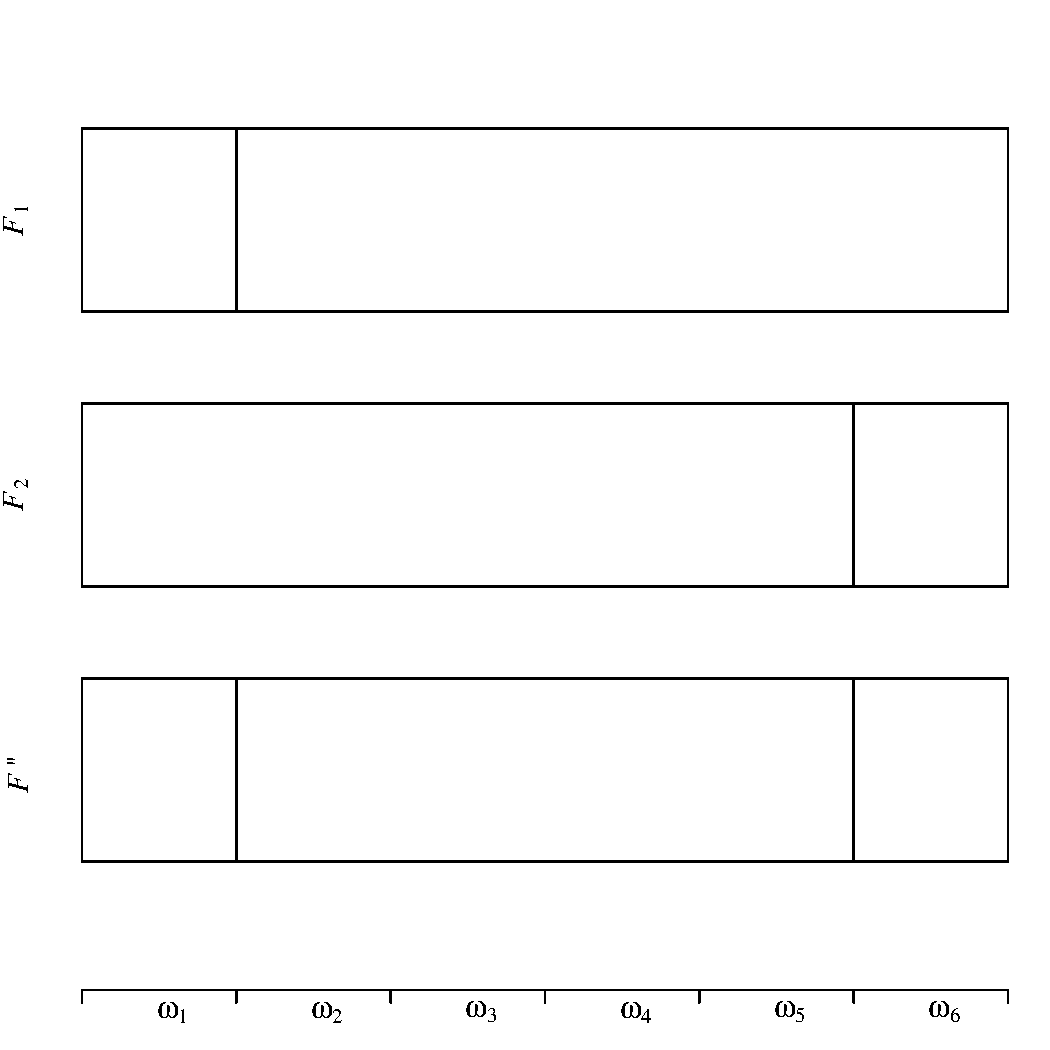
\includegraphics[width = \linewidth]{plots/Finite.pdf} % requires the graphicx package
   \caption{The information sets $\F_1$ and $\F_2$ in Example \ref{Example1} are generated by the above partitions of $\Omega = \{\omega_1, \dots, \omega_6\}$. The collected information $\F''$ is then generated by the partition induced by considering all interactions of the forecasters' partitions.}
   \label{ExamplePartitionFinite}
\end{subfigure}%
\hspace{0.7em}
\begin{subfigure}[t]{.48\textwidth}
   \centering
   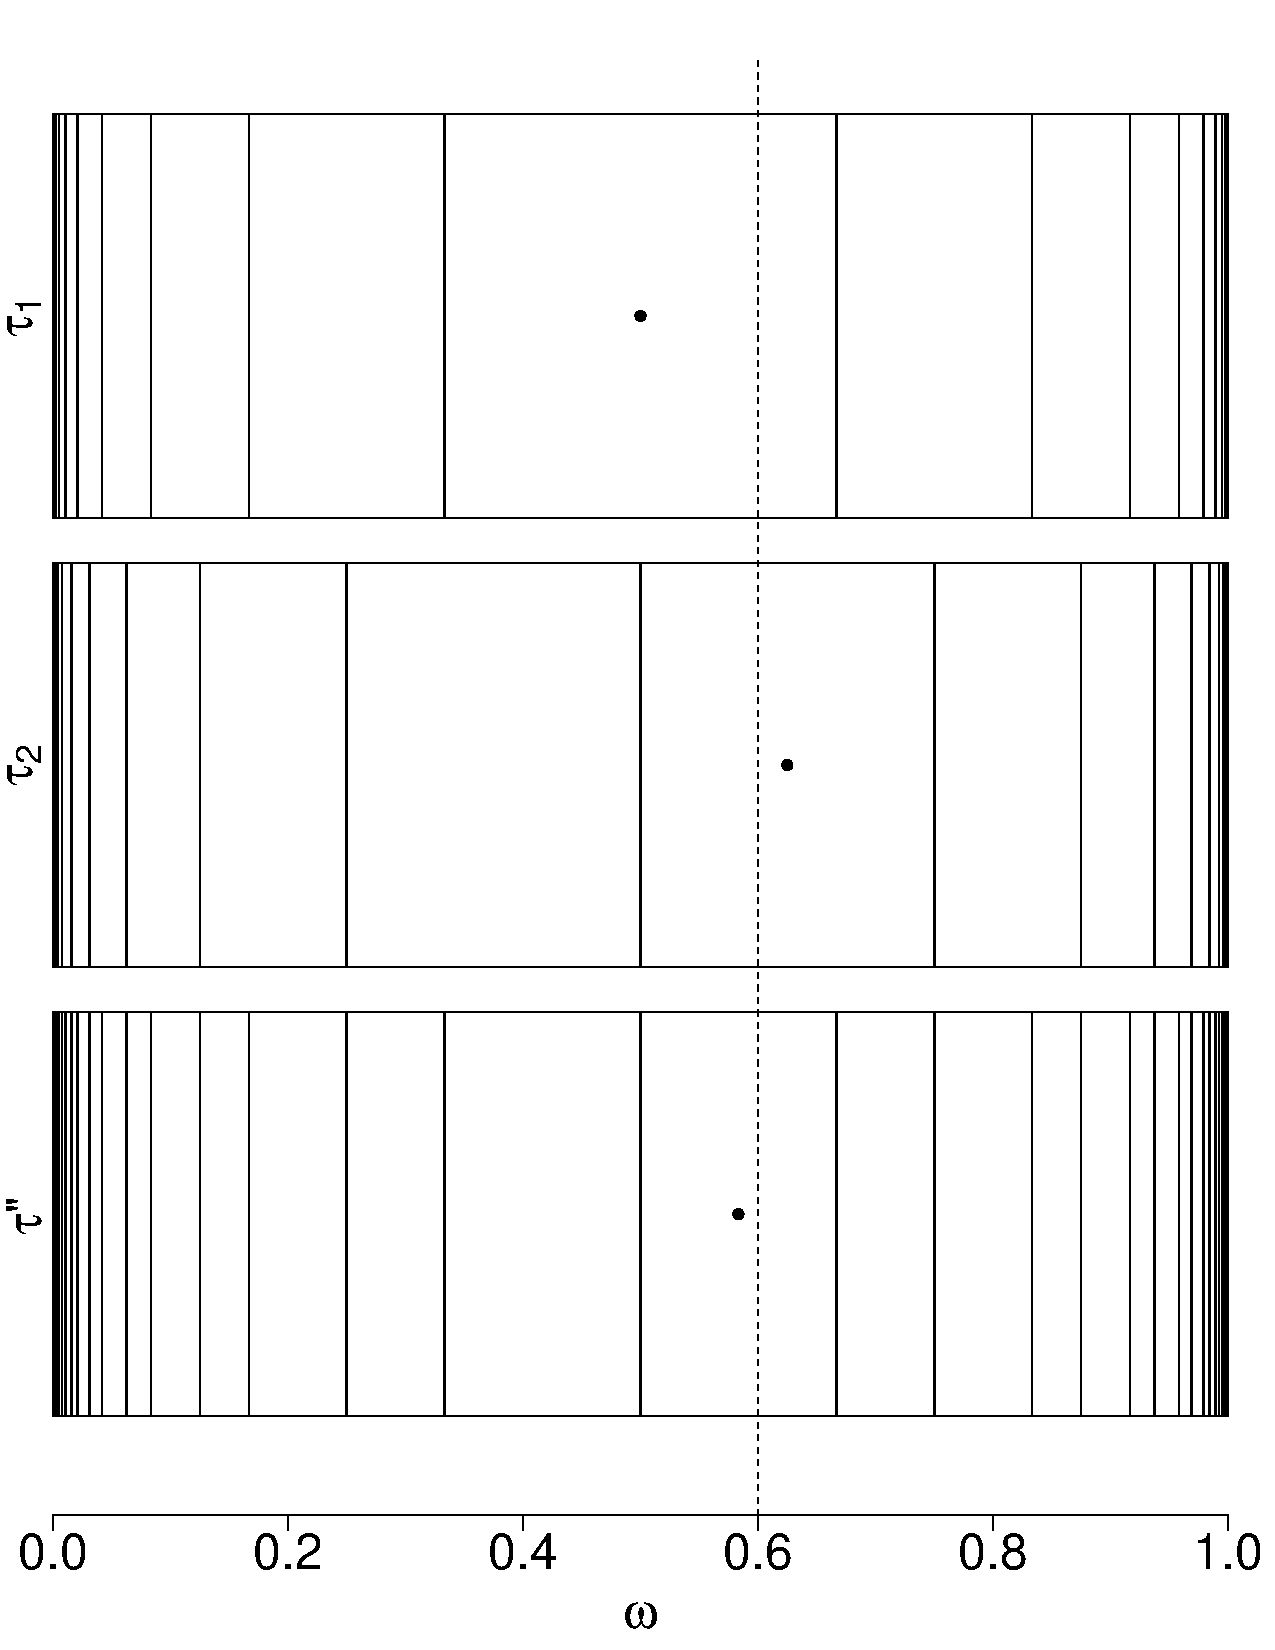
\includegraphics[width = \linewidth]{plots/Countable.pdf} % requires the graphicx package
   \caption{The partitions $\tau_1$ and $\tau_2$ generate the forecasters' information. Together they form the partition $\tau''$ that generates the revealed information. Under Lebesgue measure the forecasts are the middle points of each interval. Observe how $\mathcal{X}''$ is strictly between $X_1$ and $X_2$. }
   \label{ExamplePartition}
\end{subfigure}
\end{figure}


%\begin{figure}[t!]
%   \centering
%   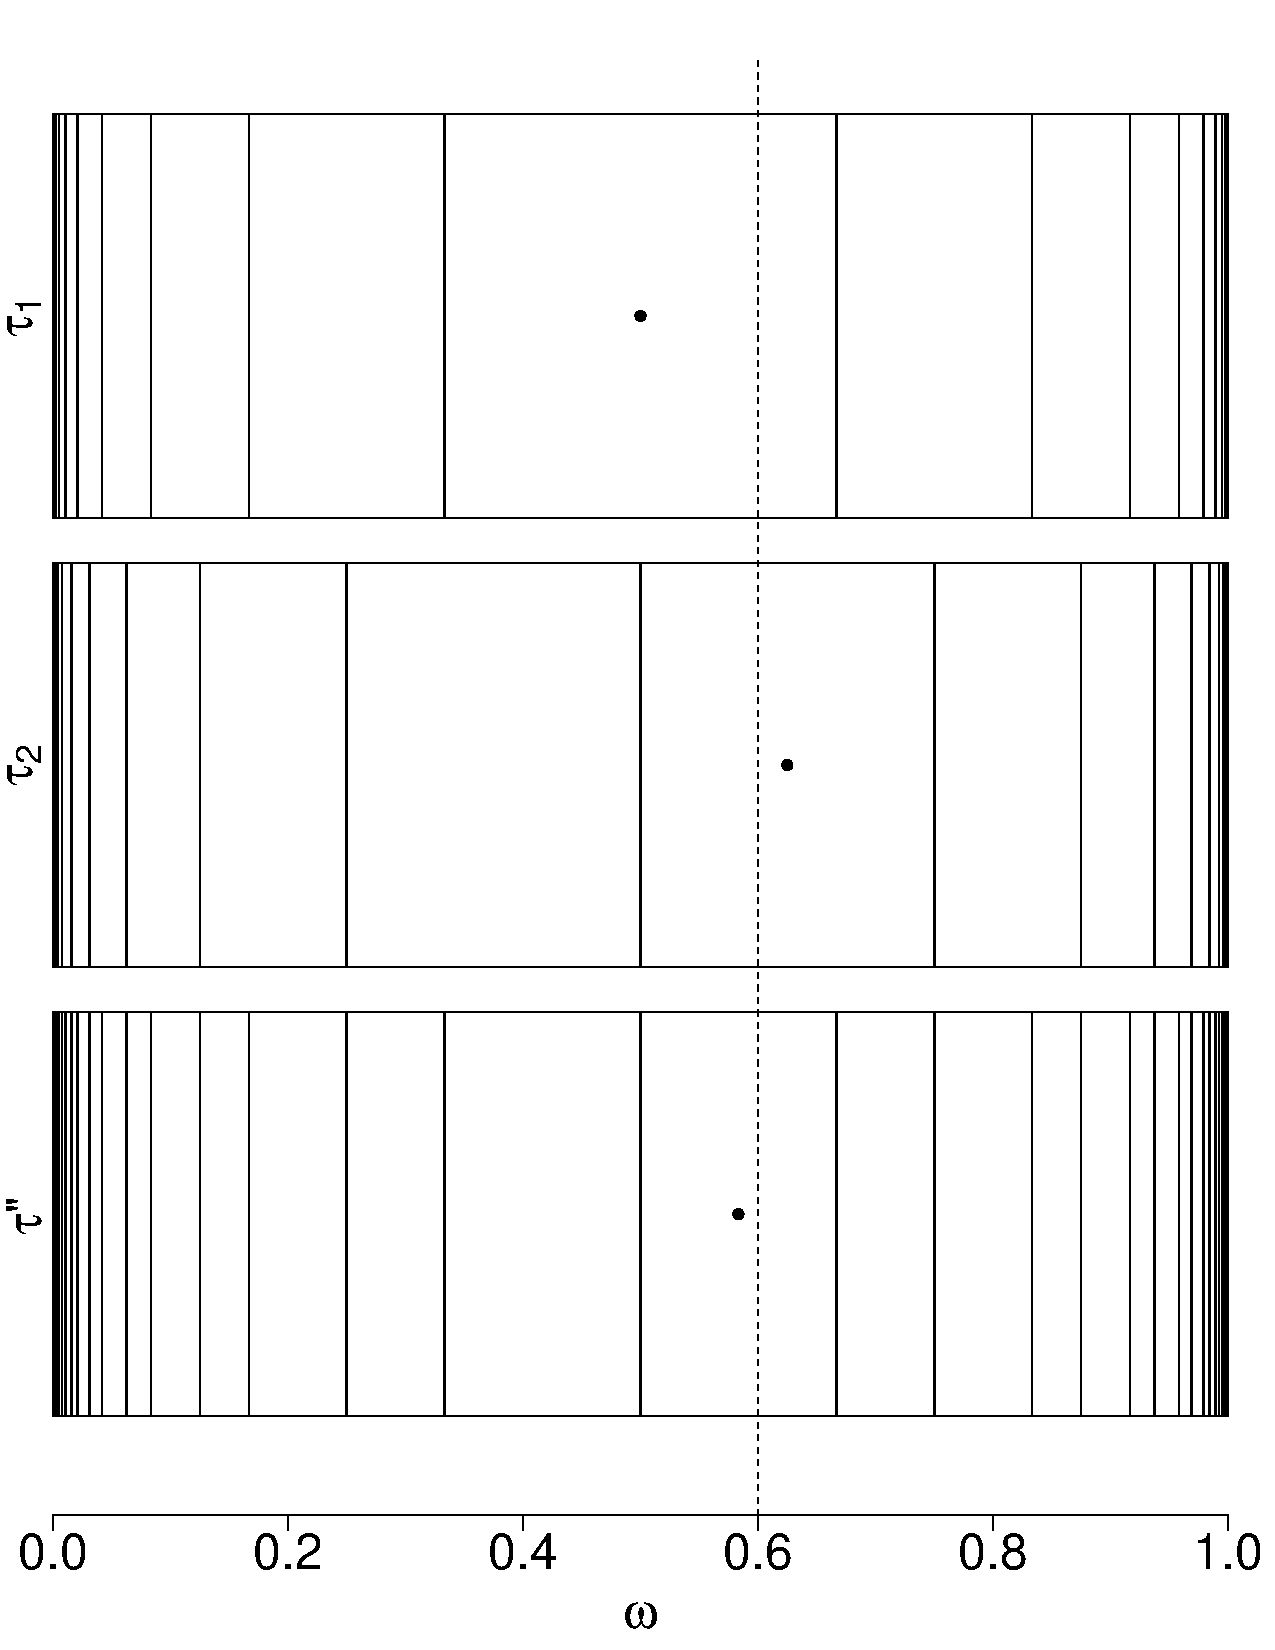
\includegraphics[width = 0.5\linewidth]{plots/Countable.pdf} % requires the graphicx package
%   \caption{The partitions $\tau_1$ and $\tau_2$ generate the forecasters' information. Together they form the partition $\tau''$ that generates the revealed information. Under Lebesgue measure the forecasts are the middle points of each interval. Observe how $X''$ is strictly between $X_1$ and $X_2$. }
%   \label{ExamplePartition}
%\end{figure}
%
%\begin{example}
%Consider a probability space $(\Omega, \F, \P)$, where $\Omega = \R$ and $\F$ is the Borel $\sigma$-field. Let the target outcome be $Y(\omega) = \omega$. Consider two forecasters with the following information sets: 
%\begin{align*}
%\F_1 &= \sigma(\dots, [-2 -1), [-1, 0), [0, 1), [1, 2), [2, 3), \dots)\\
%&= \sigma\left(A_j := [j,j+1) : j \in \mathbb{Z}\right)\\
%\F_2 &= \sigma(\dots, [-1.5, -0.5), [-0.5, 0.5), [0.5, 1.5), [1.5, 2.5), [2.5, 3.5), \dots)\\
%&= \sigma\left(B_j := [j-0.5,j+0.5) : j \in \mathbb{Z}\right)\\
%\F'' &= \sigma(\dots, [-1, -0.5), [-0.5, 0), [0, 0.5), [0.5, 1), [1, 1.5), \dots)\\
%&= \sigma\left(C_j := [j/2,j/2+0.5) : j \in \mathbb{Z}\right)
%\end{align*}
%Suppose that $\P(C_j) > 0$ for all $j \in \mathbb{Z}$. Each of these information sets is generated by a countably infinite partition of $\Omega$. This setup is illustrated in Figure . The forecasts here are 
%\begin{align*}
%X_1(\omega) = \E(Y|\F_1)(\omega) &= \sum_{i}\frac{\int_{A_i} Y d\P}{\int_{A_i}1 d\P} \one_{A_i} = \sum_{i}\frac{\E( \one_{A_i} Y )}{\P(A_i)} \one_{A_i} \text{ a.s.}\\
%X_2(\omega) = \E(Y|\F_2)(\omega) &= \sum_{j}\frac{\int_{B_j} Y d\P}{\int_{B_j}1 d\P} \one_{B_j} = \sum_{j}\frac{\E( \one_{B_j} Y )}{\P(B_j)} \one_{B_j}\text{ a.s.}\\
%X''(\omega) = \E(Y|\F'')(\omega) &= \sum_{k}\frac{\int_{C_k} Y d\P}{\int_{C_k}1 d\P} \one_{C_k} = \sum_{k}\frac{\E( \one_{C_k} Y )}{\P(C_k)} \one_{C_k}\text{ a.s.}\\
%\end{align*}
%\end{example}
%
\begin{example}
Consider a probability space $(\Omega, \F, \P)$, where $\Omega = [0,1]$, $\F$ holds all the Borel subsets of $\Omega$, and $\P$ is the Lebesgue measure. The target outcome is defined as $Y(\omega) = \omega$. Pick two strictly increasing countably infinite sequences within the unit interval
\begin{align*}
%\tau_1 &= \{\dots, a_{-3}}\} \\
\tau_1= \{\dots, a_{-2}, a_{-1}, a_0, a_1, a_2, \dots\} && \text{and} &&
%= \left\{\dots, \frac{1}{12}, \frac{1}{6}, \frac{1}{3}, \frac{2}{3}, \frac{5}{6}, \frac{11}{12}, \dots\right\} = \left\{\frac{1}{2} \pm \left( \frac{1}{6} - \frac{\gamma_k}{3} \right): k \in \mathbb{N}\right\}\\
%\tau_2 &= \{b_k :  k \in \mathbb{N}, b_k \in [0,1], b_k < b_{k+1}\} 
\tau_2= \{\dots, b_{-2}, b_{-1}, b_0, b_1, b_2, \dots\}
% = \left\{\dots, \frac{1}{8}, \frac{1}{4}, \frac{1}{2}, \frac{3}{4}, \frac{7}{8}, \dots\right\} =  \left\{\frac{1}{2}, \frac{1}{2} \pm \frac{\gamma_k}{4} : k \in \mathbb{N}\right\},
\end{align*}
such that $a_{-k} \downarrow 0$, $b_{-k} \downarrow 0$, $a_k \uparrow 1$, and $b_{k} \uparrow 1$ as $k \to \infty$. Suppose that these values alternate between the two sequences: $b_{k} < a_{k} < b_{k+1} < a_{k+1}$ for all $k \in \mathbb{Z}$. For instance, one can let
%%based on the following points:
\begin{align}
\tau_1 &= 
%\{\dots, a_{-1}, a_0, a_1, \dots\} = \left\{\dots, \frac{1}{12}, \frac{1}{6}, \frac{1}{3}, \frac{2}{3}, \frac{5}{6}, \frac{11}{12}, \dots\right\} =
 \left\{\frac{1}{2} \pm \left( \frac{1}{6} - \frac{\gamma_k}{3} \right): k \in \mathbb{N}\right\} & \text{ and } && \tau_2 &=
% \{\dots, b_{-1}, b_0, b_1, \dots\} = \left\{\dots, \frac{1}{8}, \frac{1}{4}, \frac{1}{2}, \frac{3}{4}, \frac{7}{8}, \dots\right\} =  
 \left\{\frac{1}{2}, \frac{1}{2} \pm \frac{\gamma_k}{4} : k \in \mathbb{N}\right\}, \label{specificChoice}
\end{align}
%Consider two forecasters with the following information sets: 
%\begin{align*}
%\F_1
%% &= \sigma(\dots, A_{-1}, A_0, A_1, \dots)\\
%%&= \sigma(\dots, [1/12, 1/6), [1/6, 1/3), [1/3, 2/3], (2/3, 5/6], (5/6, 11/12], \dots)\\
%&= \sigma\left(\left[2/3 - \gamma_{k+1}/3, 2/3 - \gamma_{k}/3\right), [1/3, 2/3], \left(2/3 + \gamma_{k}/3, 2/3 + \gamma_{k+1}/3\right] \right)\\
%\F_2 
%%&= \sigma(\dots, [1/16, 1/8), [1/8, 1/4), [1/4, 1/2], (1/2, 3/4], (3/4, 7/8], (7/8, 15/16], \dots)\\
%&= \sigma\left(\left[1/2 - \gamma_{k+1}/4, 1/2 - \gamma_k/4\right), [1/4, 1/2], (1/2, 3/4], \left(1/2 + \gamma_k/4, 1/2 + \gamma_{k+1}/4 \right] \right)
%%\\
%%&= \sigma\left(\left[\frac{1}{6} - \frac{1}{3}\sum_{j=0}^{k+1} \left( \frac{1}{2}\right)^j,\frac{1}{6} - \frac{1}{3}\sum_{j=0}^k \left( \frac{1}{2}\right)^j \right), \left(\frac{2}{3} + \frac{1}{3}\sum_{j=0}^{k} \left( \frac{1}{2}\right)^j,\frac{2}{3} + \frac{1}{3}\sum_{j=0}^{k+1} \left( \frac{1}{2}\right)^j \right]: k \in \mathbb{N}\right)
%\end{align*}
where $\gamma_k = \sum_{j=0}^{k} \left( \frac{1}{2}\right)^j$ and $\gamma_k \to 2$ as $k \to \infty$. These partitions are illustrated in Figure \ref{ExamplePartition}. In general, the sequences $\tau_1$ and $\tau_2$ define two countably infinite partitions of $\Omega$. The atoms of these partitions accumulate only at the extremes, and no atom in one partition is contained within an atom in the other partition.
%Given that $\gamma_k \to 2$ as $k \to \infty$, each collection forms a countably infinite partition of $\Omega$. 
Now, generate the $j$th forecaster's information set from the partition induced by $\tau_j$. This computes all possible disjoint unions of the atoms. The result is an uncountable information set because it has the same cardinality as the power set of a countably infinite set. 
%The information set then has the same cardinality as the power set, which is uncountably infinite. 
 Their combined information is generated by the partition
%\begin{align*}
$\tau'' = \{\dots, a_{-1}, b_{-1}, a_0, b_0, a_1, b_1, \dots\}$. 
%\end{align*}

 Each forecaster predicts the middle point of the atom to which the realized $\omega$ belongs. More specifically, if $\omega \in [a_j, a_{j+1}] \cap [b_i, b_{i+1}]$, then $X_1 = (a_j+a_{j+1})/2$, $X_2 = (b_i+b_{i+1})/2$, and the information collector is
\begin{align}
\mathcal{X}'' &= \begin{cases}
(b_i+a_{j+1})/2 & \text{ if } a_j < b_i\\
(b_{i+1}+a_{j})/2 & \text{ if } a_j > b_i
\end{cases}. \label{Example2Rev}
\end{align}
Given the way these points alternative in a strictly increasing manner, $\mathcal{X}''$ is always strictly between $X_1$ and $X_2$. Thus $\mathcal{X}''$ is a random strictly convex combination. Under the specific sequences (\ref{specificChoice}), the information collector (\ref{Example2Rev}) becomes
\begin{align*}
\mathcal{X}''
%&= \begin{cases}
%\frac{1}{3}X_1 + \frac{2}{3}X_2 & \text{ if } X_1 < X_2\\
%\frac{2}{3}X_1 + \frac{1}{3}X_2 & \text{ if } X_1 > X_2
%\end{cases}\\
&= \begin{cases}
\frac{2}{3} \min(X_1,X_2) + \frac{1}{3} \max(X_1,X_2) & \text{ if } X_2 < 0.5\\
\frac{1}{3} \min(X_1,X_2) + \frac{2}{3} \max(X_1,X_2) & \text{ if } X_2 > 0.5\\
\end{cases}
% \label{SpecificX}
\end{align*}
This is a weighted average of the forecasts but the weights depend on the realized values of the forecasts. In particular, a weight of $2/3$ is given to the forecast that is closer to the nearest extreme value (at $0.0$ or $1.0$). Compared to the equally weighted average $(X_1+X_2)/2$, the aggregator $\mathcal{X}''$ is then closer to the nearer extreme value, or equivalently, further away from the marginal mean $\mu_0 = \E(X_j) = 0.5$. 

% $X''(\omega) = (b_i+a_{j+1})/2$ if $a_j < b_i$ and otherwise $X''(\omega) = (b_{i+1}+a_{j})/2$ if $a_j < b_i$ 
% The revealed information is
%\begin{align*}
%\F'' &= \sigma(\dots, [1/12, 1/6), [1/4, 1/3), [1/3, 1/2], (2/3, 5/6], (5/6, 11/12], \dots)\\
%\end{align*}
%CAN YOU CHOOSE THESE SUCH THAT THE AGGREGATE IS THE GEOMETRIC MEAN.
\end{example}


%The specific partitions (\ref{specificChoice}) were chosen because they lead to an information collector (\ref{SpecificX}) that is clearly within Definition \ref{Xsc}. Therefore if $\F_j$, for $j = 1, \dots, N$, are allowed to  be uncountably large, $\mathcal{X}_{(\cdot)}$ can collect information.  


%Of course, it is possible to imagine many different examples where the information collector is a random strict convex combination. been constructed specifically such that it is clearly a reasonable measure of central tendency. Can we think of a real world example where we would give more weight to a maximum forecast?
Given that the inefficiency result (Theorem \ref{centralTendency}) does not hold under uncountably infinite $\sigma$-fields, it is natural to ask whether such $\sigma$-fields exist in the real world. Suppose, for instance, that the forecaster first observes a random variable $Z$ and then makes a prediction based on this information. If $Z$ only takes upon a finite number of different values, then the forecasters information set will be finite; that is, $|\sigma(Z)| < \infty$. If, on the other hand, $Z$ takes upon an infinite number of different values, then the information set will be uncountable. Such information sets, however, do not exist in the real-world. First, information content is finite in the physical world \citep{hibbard2014self}. In fact, according to \cite{lloyd2002computational}, the observable universe has a finite information capacity of at most $10^{120}$ bits. Second, even if the universe did contain infinite information, forecasters could not process it. Computers have finite memory and represent the world in a discrete form. For instance, consider an algorithm that makes predictions based on a dataset. There are only finitely many values this dataset can realize on the computer's finite and discrete memory. Thus the dataset generates a finite $\sigma$-field. 
%Human forecasters, however, live in a continuous world and base their forecasts on their past experience. 
%Is this realized as a infinite variable or as a finite variable? It is certainly an uncountable variable but is it processed as such by the human? 
Similarly, the human cognition is limited in its ability to process information.
% See  brain is a finite physical object, made out of a finite number of different particles. If this is considered the random variable leading to the forecast, it is finite and hence generates a finite information set. 
Therefore, even though a forecaster with infinite information may be a convenient approximation in some theoretical work, it is not a precise description of reality. For all practical purposes, this makes Theorem \ref{centralTendency} the more relevant result. The following corollary states this in terms of measures of central tendency. 
\begin{corollary}[Inefficiency of Measures of Central Tendency] \label{MCTCor}
For all practical purposes, measures of central tendency do not collect information.
\end{corollary}
This result concludes the theoretical development of this paper. The next section summarizes the results and explains how they relate to other areas of forecasting literature. 


%Consequently, in practice no measure of central tendency collects information from calibrated forecasts.
% While these arguments may seem overly philosophical, they emphasize both the highly theoretical nature of our results in Section and also the general scope of the results in Section . 
%\url{https://arxiv.org/pdf/1411.1373.pdf} 

%\marginpar{Write the final result as a corollary: only collects information if uncountable information sets}



%Another example would consider $\Omega = \R$ with Gaussian measure on it. Then we can have overlapping sets that drifts off to infinity. The aggregate must always be in the middle. 


%Explain why average here does not reduce to a fixed weight average. 

%To appreciate how subtle the difference is: Note that each countably infinite set can be modified such that the difference between the new finite set and the original countably infinite set has only measure $\epsilon > 0$. This can be made vanishing small, and hence small enough to not make a difference in practice. An average can never collect information over the modified sets but it can over the non-modified. Yet, we may not observe the difference between the forecasts in a million years. The countably infinite case is only the limiting case of the finite partition theory. 
%
%These $\sigma$-fields are actually uncountable. To see this, let $\{C_k : k =1, \dots\}$ denote the countable partition of $\Omega$. Then each $C \in \F''$ can be written as some union 


%This shows that averaging like techniques only work when people have infinite information. Is this realistic? That is what the next subsection talks about.


%\marginpar{This contradicts the Page hypothesis}


%roughly 100 million neurons and 100 billion synapses linking the neurons together. Every possible setting of these is a realization of a random variable. Given that this is a finite object with only finitely many states, the information generated by this random variable is contained in a finite $\sigma$-field. 




%\subsection{Random Strict Convex Combinations}
%\marginpar{The only assumption here is that we are assuming each sigma-field to be generated by a finite collection}
%%\textbf{Suppose that $X'' = \sum_{j=1}^N w_jX_j$ for some random $w_j \in (0,1)$ such that $\sum_{j=1}^N w_j = 1$}\\
%\textbf{Suppose that $X'' \in (\min\{X_1, \dots, X_N\}, \max\{X_1, \dots, X_N\})$ a.s.}\\
%\\
%Consider probability space $(\Omega, \F, \P)$. Suppose $\E | Y | < \infty$ and that $\F_j = \sigma(A_{ij} : i = 1, 2, \dots)$ are generated by  countable partitions of $\Omega$. The generator of the cumulative information is formed by taking all intersections $\F'' = \sigma(C_1, C_2, \dots)$.
%% It is known that every $\sigma$-field on a countable set $\Omega$ can be generated by a countable partition.  
%%Note that all of these partitions must satisfy the law of total expectation: $\E[Y] = \sum_i^I \E[Y | A_i] \P(A_i)$. This shows the overall budget. 
%% (To justify the use of a partition: \url{http://math.stackexchange.com/questions/1441596/show-the-sigma-algebra-of-a-countable-set-is-generated-by-a-partition})
%%We can merge each $w \in C_{ij}$ into a single $w$ with the combined measured because none of the observables change if one moves from one $w$ to another within the same $C_{ij}$. Therefore we can assume that each $C_{ij}$ holds only one $w$. 
%Observe that $X_j$ remains constant over any set $A_{ij}$. The set $A_{ij}$ can be written as a unique union of some $C_k$'s. More specifically, 
%\begin{align*}
%X_j(A_{ij}) = \frac{\sum_{\omega \in A_{ij}} \P(\omega) Y(\omega)}{\sum_{\omega \in A_{ij}} \P(\omega)} &= \frac{\sum_{k : C_k \cap A_{ij} \neq \emptyset}\sum_{\omega \in C_k} \P(\omega) Y(\omega)}{\sum_{\omega \in A_{ij}} \P(\omega)}\\
% &= \frac{\sum_{k : C_k \cap A_{ij} \neq \emptyset}X''(C_k) \sum_{\omega \in C_k} \P(\omega) }{\sum_{\omega \in A_{ij}} \P(\omega)}\\
% &= \sum_{k : C_k \cap A_{ij} \neq \emptyset}p_{ijk}X''(C_k),
%\end{align*}
%where $p_{ijk} = \sum_{\omega \in C_k} \P(\omega)  / \sum_{\omega \in A_{ij}} \P(\omega)$ such that $\sum_{k : C_k \cap A_{ij} \neq \emptyset}p_{ijk} = 1$. 
%%Given that the weights $w_j \in (0,1)$, $X''$ is always in the interior of the convex hull of the forecasts; that is, $X''(\omega) \in (\min\{X_j(\omega)\}, \max\{X_j(\omega)\})$. 
%Note that all forecasts remain constant over any set $C_k$. 
%Hence it is sufficient to consider the sets $C_k$ instead of the individual $\omega$'s. Define the index for the minimum forecast over a set $C_k$ as ${j}^* := \argmin_j\{X_j(C_k)\}$ and index for the maximum forecast as $j^{**} := \argmax_j\{X_j(C_k)\}$. Given that $X''$ is always in the interior of the convex hull of the forecasts, for all sets $C_k$, we have that
%% Similarly define $q_{jk} = \sum_{w \in C_k} \P(w)  / \sum_{w \in B_j} \P(w)$. 
%% and hence would contradict our assumption.
%%\scriptsize
%\begin{align*}
%X_{j^*}(C_{k}) &< X''(C_{k}) < X_{j^{**}}(C_{k})\\
%\Leftrightarrow \sum_{k' : C_k \cap A_{ij^*} \neq \emptyset, C_{k'} \cap A_{ij^*} \neq \emptyset}p_{ij^*k'}X''(C_{k'}) &<  X''(C_k)  <   \sum_{k' : C_k \cap A_{ij^{**}} \neq \emptyset, C_{k'} \cap A_{ij^{**}} \neq \emptyset}p_{ij^{**}k'}X''(C_{k'})\\
%%\frac{\sum_{w \in  A_1 / C_{11}} \P(w) Y(w) + \sum_{w \in C_{11}} \P(w) Y(w)}{\sum_{w \in A_1} \P(w)} &< \frac{\sum_{w \in C_{11}} \P(w) Y(w)}{\sum_{w \in C_{11}} \P(w)}  < \frac{\sum_{w \in B_1 / C_{11}} \P(w) Y(w) + \sum_{w \in C_{11}} \P(w) Y(w)}{\sum_{w \in B_1} \P(w)}\\
%%\frac{\sum_{w \in  A_1 / C_{11}} \P(w) Y(w) + X''(w_1)  \sum_{w \in C_{11}} \P(w) }{\sum_{w \in A_1} \P(w)} &< X''(w_1)   < \frac{\sum_{w \in B_1 / C_{11}} \P(w) Y(w) + X''(w_1)  \sum_{w \in C_{11}} \P(w) }{\sum_{w \in B_1} \P(w)}\\
%%\frac{\sum_{w \in  A_1 / C_{11}} \P(w) Y(w) +   \sum_{w \in C_{11}} \P(w) X''(w_1) }{\sum_{w \in A_1} \P(w)} &< X''(w_1)   < \frac{\sum_{w \in B_1 / C_{11}} \P(w) Y(w) +   \sum_{w \in C_{11}} \P(w) X''(w_1)}{\sum_{w \in B_1} \P(w) }
%\Leftrightarrow \max L_k &< X''(C_k)  < \min U_k,
%\end{align*}
%where
%\begin{align*}
%L_k := \{X''(C_{k'}) : X''(C_{k'}) < X''(C_{k}), C_k \cap A_{ij^*} \neq \emptyset, C_{k'} \cap A_{ij^*} \neq \emptyset\}\\
% U_k := \{X''(C_{k'}) : X''(C_{k'}) < X''(C_{k}), C_k \cap A_{ij^{**}} \neq \emptyset, C_{k'} \cap A_{ij^{**}} \neq \emptyset\} 
%\end{align*}
%Given that $X''(C_k)$ is included on both sides of the strict inequality, we know that $L_k$ and $U_k$ are non-empty. They can be finite or countable.  
%
%\noindent
%\textbf{Countable partitions:} If this is true, then $X''$ must be bounded from below and above by limit points. That is, there is some (potentially infinite) lower bound $l$ such that $X''(C_k) \downarrow l$ monotonically as $k \to \infty$ for some sets of the partition and similarly for an upper bound $X''(C_k) \uparrow u$ monotonically. Note that for each $X''(C_k)$ there is some $X_j$ that is strictly greater (or lower) than $X''(C_k)$.  
%
%%Note that
%%\begin{align*}
%%X''(C_k) &= \sum_{j=1}^N w_j X_j(C_k)\\
%%&= \sum_{j=1}^N w_j X_j(A_{ij} : A_{ij} \cap C_k \neq \emptyset)\\
%%&= \sum_{j=1}^N  \sum_{k' : C_{k'} \cap A_{ij} \neq \emptyset, C_{k} \cap A_{ij} \neq \emptyset} w_j p_{ijk'}X''(C_{k'})
%%\end{align*}
%%Hence each $X''(C_k)$ is a convex combination of some other $X''(C_k)$'s.  Here each $w_j \in (0,1)$ but each $p_{ijk'} \in [0,1]$. Thus $w_jp_{ijk'} \in [0,1)$. They all sum to one. This suggests that at least two difference $X''(C_k)$'s are used in this composition. 
%
%
%\noindent
%\textbf{Finite partitions:} This is a set of $K$ inequalities. In particular, it gives strict upper and lower bounds for each $X''(C_k)$ in terms of the other $X''(C_k)$; that is, each $X''(C_k)$ is upper and lower bounded by some other $X''(C_k)$. This, however, necessarily leads to a cycle of strict inequalities of the form $X''(C_{(1)}) < X''(C_{(2)}) < \dots < X''(C_{(1)})$. To see this, consider a set of $K$ elements $\{x_1, \dots, x_K\}$ in which for each $x_j$ there is some $x_k$ such that $x_j < x_k$ and $j \neq k$. Thus one can begin with a element, say, $x_1$ and always move to another element that is strictly greater. Unfortunately, however, one can make at most $K-1$ steps before the next strictly increasing element is an element that has already been visited. Thus the current element is both strictly smaller and greater than that element. This is a contradiction. Thus such inequalities cannot hold simultaneously. 
%
%\marginpar{When do you have a generator for the sigma field?}
%\marginpar{This assumes a finite partition? Does this need to be the case?}
%%\marginpar{What about equal sets or border case sets? What do we need for this proof to work? Is it enough to just stay that X'' is always strictly inside the convex hull of the forecasts.}
%\marginpar{Should we re-write this with integration?}



%, however, is not possible because it implies, for instance, that there is no minimum $X''(C_k)$. 

%\normalsize
%This tells us that $\min\{X''(C_k) : C_k \cap A_1 \neq \emptyset\} < X''(C_1) < \max\{X''(C_k) : C_k \cap B_1 \neq \emptyset\}$. Now if the sets are contiguous, then (again it does not matter how we label)
%\begin{align*}
%p_{11}X''(C_1) + p_{1K}X''(C_{K}) &< X''(C_1)  <  q_{11}X''(C_1)  + q_{12}X''(C_{2}),
%\end{align*}
%which then gives that $X''(C_K) < X''(C_1) < X''(C_2)$. Now repeat this argument for $C_2$ to get that $X''(C_3) < X''(C_2) < X''(C_1)$ (if $X_1(C_2) < X_2(C_2)$)  or $X''(C_1) < X''(C_2) < X''(C_3)$ (if $X_1(C_2) > X_2(C_2)$). Of course, based on what we know from before, only the second case is possible. Hence we have established that $X''(X_K) < X''(C_1) < X''(C_2) < X''(C_3)$. You repeat this argument until the very last set. This then gives you $X''(C_{K-1}) < X''(C_K)$. A contradiction. 





%\subsection{Random Weighted Averaging: Calibration}
%
%The goal in this section is to analyze the (random) weighted average and in particular show that it does not collect information. To keep things tractable, suppose we are working in $L^2(\Omega, \F, \P)$. This is a Hilbert space with all random variables $X \in \F$ such that $\int_\Omega |X|^2 d\P = \E(|X|^2) < \infty$. The inner product is $\langle X,Y \rangle = \E (XY)$. The norm is $||X||^2 = \int_\Omega X^2 d\P = \E(X^2)$. Recall that a Hilbert space is a Banach space; hence every Cauchy sequence converges to an element in the same space. This is important for taking limits. By making this assumption, we are assuming that the outcome $Y$ has $\E(Y^2) < \infty$. 
%
%The Cauchy-Schwartz inequality says that $|\langle X,Y \rangle| \leq \sqrt{\langle X,X \rangle \langle Y,Y \rangle}$. This shows that $-1 \leq \langle X,Y \rangle  / \sqrt{\langle X,X \rangle \langle Y,Y \rangle} \leq 1$, which means that we can interpret it as the cosine of the angle between $X$ and $Y$. Note that if the random variables are assumed to have mean zero, then  $ \langle X,Y \rangle  / \sqrt{\langle X,X \rangle \langle Y,Y \rangle}  =  \E (XY) / \sqrt{ \E (X^2)  \E (Y^2)} = \Corr(X,Y)$
%
%
%%In this vector space, the length $||X||$ is the standard deviation of $X$. 
%
%Any conditional expectation $X_j = \E(Y|\F_j)$ with $\F_j \subset \F$ is an orthogonal projection of $Y$ onto the space of square-integrable random variables measurable with respect to $\F_j$. Call this space $L^2(\F_j)$. Under a Hilbert space such projections are linear contractions. In other words, if $PY = \E(Y|\F_j)$, then $P(\alpha X + \beta Y) = \alpha PX + \beta PY$ and $||\E(Y|\F_j) || =  ||PY|| = \E[(PY)^2] \leq ||Y|| = \E(Y^2)$. These can be easily verified for the conditional expectation. In terms of properties of the projection,  The projections are self-adjoint: for all $X,Y \in L^2$, we have that $\langle PX, Y \rangle = \langle PX, PY \rangle  = \langle X, PY \rangle $.  The projection is idempotent; that is, $P^2 = P$. That is, projecting twice is the same as projecting once. 
%%\item 
%%The converse is also true: if $P$ is a self-adjoint operator in a Hilbert space and if $P^2 = P$, then the range of $P$ is a subspace of the Hilbert space and $P$ is a projection onto that subspace. Thus, an operator is a projection in a Hilbert space if and only if it is self-adjoint and idempotent. Note, however, that not all projections are conditional expectations. In fact, a projection $P$ on $L^2$ is a conditional expectation if and only if it is positive and it leaves the constant function $1$ invariant.   
%An operator on $L^2$ is a conditional expectation if and only if  
%\begin{enumerate}[i)]
%\item preserves unity: $P(1) = 1$. This suggests that $P$ keeps all the constants. 
%\item positive: $PX \geq 0$ for all $X \geq 0$. 
%\item linear operator: $P(\alpha X + \beta Y) = \alpha P X + \beta P Y$ for all possible $X,Y \in L^2$ and constants $\alpha, \beta$. 
%\item idempotent: $P^2 = P$, which means that multiple applications do not change the value beyond the initial application. 
%\item has $||P|| \leq 1$. 
%\end{enumerate}
%
%
%%\item Given that $P$ is self-adjoint, we have that $||P|| = 1$ where the operator is defined as 
%%\begin{align*}
%%||P|| &= \sup_{||Y||^2 = 1} |\langle PY,Y\rangle|\\
%%&= \sup_{||Y||^2 = 1} |\langle PY,PY\rangle|\\
%%&= \sup_{||Y||^2 = 1} | \E(X_j^2)|\\
%%%&= \sup_{ \E(Y^2) = 1} |\E [\E(Y | \F_j) Y]|\\
%%%&= \sup_{ \E(Y^2) = 1} |\E [X_j Y]|\\
%%%&= \sup_{ \E(Y^2) = 1} |\Cov(X_j,Y) + \mu_0^2|\\
%%\end{align*}
%
%%\item 
%%
%%\end{enumerate}
%
%
%
%The study here focuses on $\sum_{j=1}^n w_j X_j$, where each $X_j = \E(Y|\F_j)$ and $\sum_{j=1}^N w_j = 1$. The weights are assumed to be a function of $\{X_j : j = 1, \dots, N\}$ and hence random. Given that each $X_j$ is a function of $Y$, this means that the random weighted average is only a function of $Y$. This aggregator satisfies the following properties:
%
%\begin{enumerate}[i)]
%\item preserves unity: $\phi(1 | \F_1, \dots, \F_N) = \sum_{j=1}^n w_j \E(1|\F_j) = \sum_{j=1}^n w_j  = 1$
%\item positive: If $Y > 0$, then each $\E(Y | \F_j) > 0$. Given that $w_j \in [0,1]$, we have that
%\begin{align*}
%\phi(Y) &=  \sum_{j=1}^n w_j(Y; \F_1, \dots, \F_N) \E( Y|\F_j) \geq 0
%%&=  \alpha \sum_{j=1}^n w_j(\alpha Y_1 + \beta Y_2; \F_1, \dots, \F_N) \E( Y_1 |\F_j) + \beta \sum_{j=1}^n w_j(\alpha Y_1 + \beta Y_2; \F_1, \dots, \F_N) \E(Y_2|\F_j)\\\\
%\end{align*}
%
%
%\item linear operator: \\
%$\Rightarrow$ Suppose $w_j$ is a constant.  Then,
%\begin{align*}
%\phi(\alpha Y_1 + \beta Y_2) &=  \sum_{j=1}^n w_j \E(\alpha Y_1 + \beta Y_2|\F_j)\\
%&=  \sum_{j=1}^n w_j\left[ \alpha \E(Y_1| \F_j) + \beta \E(Y_2|\F_j) \right]\\
%&=   \alpha \sum_{j=1}^n w_j \E(Y_1| \F_j) + \beta \sum_{j=1}^n w_j \E(Y_2|\F_j) \\
%&= \alpha \phi( Y_1) + \beta \phi(Y_2) 
%%&=  \alpha \sum_{j=1}^n w_j(\alpha Y_1 + \beta Y_2; \F_1, \dots, \F_N) \E( Y_1 |\F_j) + \beta \sum_{j=1}^n w_j(\alpha Y_1 + \beta Y_2; \F_1, \dots, \F_N) \E(Y_2|\F_j)\\\\
%\end{align*}
%$\Leftarrow$ Suppose $\phi$ is a linear operator. Then for all $Y_1, Y_2 \in L^2$ we have that 
%\begin{align*}
%\phi(\alpha Y_1 + \beta Y_2) &=   \alpha \phi( Y_1) + \beta \phi(Y_2) \\
%\sum_{j=1}^n w_j(\alpha Y_1 + \beta Y_2) \E(\alpha Y_1 + \beta Y_2|\F_j) &= \alpha \sum_{j=1}^n w_j(Y_1) \E(Y_1| \F_j) + \beta \sum_{j=1}^n w_j(Y_2) \E(Y_2|\F_j) \\
%\sum_{j=1}^n w_j(\alpha Y_1 + \beta Y_2) \left( \alpha\E( Y_1 |\F_j)  + \beta \E(Y_2 | \F_j)\right)&= \alpha \sum_{j=1}^n w_j(Y_1) \E(Y_1| \F_j) + \beta \sum_{j=1}^n w_j(Y_2) \E(Y_2|\F_j) 
%\end{align*}
%Re-ordering the terms gives
%\begin{align*}
%\sum_{j=1}^n \left[ w_j(\alpha Y_1 + \beta Y_2) - w_j(Y_1) \right] \alpha\E( Y_1 |\F_j) + \sum_{j=1}^n \left[ w_j(\alpha Y_1 + \beta Y_2) - w_j(Y_2)\right] \beta \E(Y_2|\F_j)&= 0
%\end{align*}
%This equation has one solution at $w_j(\alpha Y_1 + \beta Y_2) = w_j(Y_1) = w_j(Y_2)$ for all $j = 1, \dots, N$. This shows that the weight functions are constant: they are the same no matter what $Y \in L^2$ is being predicted. When is this the unique solution? All solutions must work for all choices of $\{ \F_j : j = 1, \dots, N\}$ and $\alpha$. We need a subset on which only constant weights work. Setting $\beta = 0$ gives
%\begin{align*}
%\sum_{j=1}^n \left[ w_j(\alpha Y) - w_j(Y) \right] \alpha\E( Y |\F_j) &= 0\\
%\sum_{j=1}^n \left[ w_j(\alpha Y) - w_j(Y) \right] \E( Y |\F_j) &= 0
%\end{align*}
%This does not prove that the functions are constant. It only shows that they are invariable to the choice of units. For instance, think of a weight function that sets $w_j = X_j / (X_1 + \dots + X_N)$. These are random, sum to one, and also invariable to multiplications by a constant. Therefore this is not enough for us to show that the weight functions are constant. Notice, however, that the above weight function does not pass the addition test. This is quite easy to see. What kind of weights would satisfy this? Setting $\alpha = \beta = 1$ gives us
%\begin{align*}
%\sum_{j=1}^n \left[ w_j( Y_1 +  Y_2) - w_j(Y_1) \right] \E( Y_1 |\F_j) + \sum_{j=1}^n \left[ w_j( Y_1 +  Y_2) - w_j(Y_2)\right]  \E(Y_2|\F_j)&= 0
%\end{align*}
%or alternatively
%\begin{align*}
%\sum_{j=1}^n w_j( Y_1 +  Y_2) \left[ \E( Y_1|\F_j)  +  \E(Y_2|\F_j) \right] &=  \sum_{j=1}^n \left[ w_j(Y_1) \E(Y_1| \F_j) + w_j(Y_2) \E(Y_2|\F_j)  \right]
%\end{align*}
%%Looking at each term gives us 
%%
%%\begin{align*}
%%w_j( Y_1 +  Y_2) \left[ \E( Y_1|\F_j)  +  \E(Y_2|\F_j) \right] &= w_j(Y_1) \E(Y_1| \F_j) + w_j(Y_2) \E(Y_2|\F_j)\\
%%w_j( Y_1 +  Y_2) &= w_j(Y_1) \frac{\E(Y_1| \F_j)}{\left[ \E( Y_1|\F_j)  +  \E(Y_2|\F_j) \right] } + w_j(Y_2) \frac{\E(Y_2|\F_j)}{\left[ \E( Y_1|\F_j)  +  \E(Y_2|\F_j) \right] }\\
%%\end{align*}
%
%
%It is important to note here that this is a general statement about the operator. Hence it must hold for any $N$ and $\alpha, \beta$. For instance, let $Z = \alpha Y+\beta$. Then, we must also have 
%\begin{align*}
%\phi( Z) &= \alpha \phi( Y) +\beta\\
%w(Z)\E(\alpha Y+\beta | \F_1) + (1-w(Z))\E(\alpha Y+\beta| \F_2) &= w(Y)\alpha \E(Y | \F_1) + (1-w(Y))\alpha\E( Y| \F_2) + \beta\\
%w(Z) \left( \E( Y | \F_1) - \E( Y| \F_2) \right) &= w(Y) \left( \E(Y | \F_1) - \E( Y| \F_2) \right)\\
%w(\alpha Y + \beta)  &= w(Y),
%\end{align*}
%which shows that $\w(\cdot)$ is invariant to linear transformations. It is important to think about what the weight function really is. It is really a function of $X_j$ as this is what has been observed. Thus one could write $w(X_1, \dots, X_N)$. This result then shows that $w(X_1, \dots, X_N) = w(\alpha X_1 + \beta, \dots, \alpha X_N + \beta)$. In other words, the weight function is invariable to linear transformation of the forecasts. For instance, the median behaves like this. Now, let $Z = Y_1 + Y_2$. Then,
%\begin{align*}
%\phi( Y_1 + Y_2) &= \phi( Y_1) + \phi(Y_2)\\
%w(Z)\E(Z | \F_1) + (1-w(Z))\E(Z| \F_2) &= w(Y_1)\E(Y_1 | \F_1) + (1-w(Y_1))\E(Y_1| \F_2) + w(Y_2)\E(Y_2 | \F_1) + (1-w(Y_2))\E(Y_2| \F_2)
%\end{align*}
%
%%Suppose now that $Y$ is not identically zero. In fact, if $Y = 0$, there is not much forecasting to be done. Differentiating (this places some continuity constraints on $w(\cdot)$) both sides by $\alpha$ gives  $Y \frac{\partial }{\partial \alpha} w(\alpha Y) = 0$. If $Y$ is not identically zero, then $ \frac{\partial }{\partial \alpha} w(\alpha Y) = 0$. Next, differentiate both sides by $Y$ to get $\alpha \frac{\partial }{\partial Y} w(\alpha Y) = \frac{\partial }{\partial Y} w(Y)$
%
%
%%\begin{align*}
%%\phi( Y_1 + Y_2) &= \phi( Y_1) + \phi( Y_2)\\
%%%& w\E(\alpha Y_1 + \beta Y_2 | \F_1) + (1-w)\E(\alpha Y_1 + \beta Y_2 | \F_2) \\
%%% &= \alpha[w\E(Y_1 | \F_1) + (1-w)\E(Y_1 | \F_2)]+ \beta[w\E(Y_2 | \F_1) + (1-w)\E(Y_2 | \F_2)]\\
%%%& w\E(\alpha Y_1 + \beta Y_2 | \F_1) + \E(\alpha Y_1 + \beta Y_2 | \F_2) - w\E(\alpha Y_1 + \beta Y_2 | \F_2)\\
%%%  &= \alpha w\E(Y_1 | \F_1) + \alpha\E(Y_1 | \F_2) - \alpha w \E(Y_1 | \F_2)+ \beta w\E(Y_2 | \F_1) + \beta\E(Y_2 | \F_2)] - \beta w \E(Y_2 | \F_2)]\\
%%%& w\E(\alpha Y_1 + \beta Y_2 | \F_1) - w\E(\alpha Y_1 + \beta Y_2 | \F_2)  -  \alpha w\E(Y_1 | \F_1) + \alpha w \E(Y_1 | \F_2) - \beta w\E(Y_2 | \F_1) + \beta w \E(Y_2 | \F_2)]\\
%%% &= \alpha\E(Y_1 | \F_2) + \beta\E(Y_2 | \F_2)] - \E(\alpha Y_1 + \beta Y_2 | \F_2)\\
%%%& w\left( \E(\alpha Y_1 + \beta Y_2 | \F_1) - \E(\alpha Y_1 + \beta Y_2 | \F_2)  -  \alpha \E(Y_1 | \F_1) + \alpha \E(Y_1 | \F_2) - \beta \E(Y_2 | \F_1) + \beta  \E(Y_2 | \F_2)] \right)\\
%%% &= \alpha\E(Y_1 | \F_2) + \beta\E(Y_2 | \F_2)] - \E(\alpha Y_1 + \beta Y_2 | \F_2)\\
%%\end{align*}
%%which gives
%%\begin{align*}
%%w &= \frac{\alpha\E(Y_1 | \F_2) + \beta\E(Y_2 | \F_2) - \E(\alpha Y_1 + \beta Y_2 | \F_2)}{\left( \E(\alpha Y_1 + \beta Y_2 | \F_1) - \E(\alpha Y_1 + \beta Y_2 | \F_2)  -  \alpha \E(Y_1 | \F_1) + \alpha \E(Y_1 | \F_2) - \beta \E(Y_2 | \F_1) + \beta  \E(Y_2 | \F_2)] \right)}
%%\end{align*}
%%We also have the sum constraints. THIS MAY BE COMPLICATED TO SHOW.
%
%\item Idempotent: This applies the procedure twice recursively. In words, the average forecast should be the same as the average of the forecasters' predictions about the consensus. This requires the forecasters to make predictions about each others forecasts: that is, compute $\E[\E[Y| \F_i] | \F_j]$. Of course, if one $\sigma$-field is subset of the other, this can be reduced by the "smallest $\sigma$-field wins"-theorem. Typically, however, these $\sigma$-fields are partially overlapping. 
%
%\end{enumerate}
%
%
%Note that each projection $P$ on  $X, Y \in L^2$ we have that $\langle PX, Y \rangle = \langle X, PY \rangle$; that is, they are self-adjoint. The goal now is to show that this is not true for the weighted average. 
%
%\begin{align*}
%\E \left[ X \sum_{j=1}^n w_j(Y) \E(Y|\F_j) \right] &= \E \left[ Y \sum_{j=1}^n w_j(X) \E(X|\F_j) \right] \\
%\E \left[ X \sum_{j=1}^n w_j(Y) \E(Y|\F_j) \right] &= \E \left[ Y\right] \E[X]\\
%\E \left[ \sum_{j=1}^n w_j(Y) \E(Y|\F_j) \right] &= \E \left[ Y\right]\\
%\end{align*}
%The same applies for any constant $Y$. 
%
%
%\subsection{Random Weighted Averaging: Variance Bound}
%
%In this section we are analyzing the variance of $\phi(Y) = \sum_{j=1}^n w_j X_j$. In particular, the goal is to show that this variance is upper bounded by $\delta_{max} = \Var(X_{max})$. To begin, suppose $\phi$ is calibrated. If it is not, then it is not consistent with some information set and we are done. Recall that calibration implies marginal consistent. Hence $\E\phi = \mu_0$. Then,
%\begin{align*}
%\Var\left(\sum_j w_j X_j\right) &= \E\left[ \left(\sum_j w_j X_j\right)^2\right] -\mu_0^2
%\end{align*}
%Given that $\Var(X_{max}) = \E(X_{max}^2) - \mu_0^2$, it suffices to show that 
%\begin{align*}
%\E\left[ \left(\sum_j w_j X_j\right)^2\right] \leq \E(X_{max}^2)
%\end{align*}
%By Jensen's inequality, for any $\omega \in \Omega$, we have that 
%\begin{align*}
% \sum_j w_j X_j^2 -  \left(\sum_j w_j X_j\right)^2 &= \frac{1}{2}\sum_{ij} w_i w_j (X_i - X_j)^2 \\
% \left(\sum_j w_j X_j\right)^2 &=  \sum_j w_j X_j^2 - \frac{1}{2}\sum_{ij} w_i w_j (X_i - X_j)^2 \\
% \left(\sum_j w_j X_j\right)^2 &\leq  \sum_j w_j X_j^2
%\end{align*}
%Taking expectations gives us
%\begin{align*}
% \E \left(\sum_j w_j X_j\right)^2 &=  \sum_j \E (w_j X_j^2) - \frac{1}{2}\sum_{ij} \E[w_i w_j (X_i - X_j)^2]\\
% &=  \sum_j \E (w_j) \E(X_j^2) + \Cov(w_j, X_j^2) - \frac{1}{2}\sum_{ij} \E[w_i w_j (X_i - X_j)^2]\\
% &\leq \sum_j \E (w_j) \E(X_{max}^2) + \sum_j\Cov(w_j, X_j^2) - \frac{1}{2}\sum_{ij} \E[w_i w_j (X_i - X_j)^2]\\
% &=  \E(X_{max}^2) + \sum_j\Cov(w_j, X_j^2) - \frac{1}{2}\sum_{ij} \E[w_{i}w_j (X_i - X_j)^2]
%% &=  \E(X_{max}^2) + \sum_j\Cov(w_j, X_j^2) - \sum_{i<j} \E[w_{ij} (X_i - X_j)^2],
%\end{align*}
%%where $w_{ij} = w_i w_j \leq \min\{w_i, w_j\}$.  
%%This inequality is sharp, with the equality happening when $X_i = X_j$ for all $i \neq j$. Note also that it is trivially true for constant $w_j$ or if $w_j$ is uncorrelated with $X_j$ because in both cases all $\Cov(w_j, X_j^2) = 0$. 
%Therefore it remains to be shown that 
%\begin{align*}
%\sum_j\Cov(w_j, X_j^2) &\leq \frac{1}{2}\sum_{ij} \E[w_{i}w_j (X_i - X_j)^2] \\
%%\sum_j \E[w_j X_j^2] - \sum_j \E[w_j]\E[X_j^2] &\leq \frac{1}{2}\sum_{ij} \E[w_{i}w_j (X_i - X_j)^2] \\
%\E[ \sum_{ij}w_iw_j X_j^2] - \sum_j \E[w_j]\E[X_j^2] &\leq \frac{1}{2}\sum_{ij} \E[w_{i}w_j (X_i - X_j)^2] \\
%\E[ \sum_{ij}w_iw_j X_j^2] - \sum_j \E[w_j]\E[X_j^2] &\leq \frac{1}{2}\left( \sum_{ij} \E[w_{i}w_j X_i^2 - 2w_{i}w_j X_iX_j + w_{i}w_jX_j^2]  \right) \\
%\E[ \sum_{ij}w_iw_j X_j^2] - \sum_j \E[w_j]\E[X_j^2] &\leq \left( \sum_{ij} \E[w_{i}w_j X_i^2 - w_{i}w_j X_iX_j]  \right) \\
% - \sum_j \E[w_j]\E[X_j^2] &\leq - \sum_{ij} \E[w_{i}w_j X_iX_j]   \\
%\E\left[ (\sum_j w_j X_j)^2 \right] = \sum_{ij} \E[w_{i}w_j X_iX_j]   &\leq   \sum_j \E[w_j]\E[X_j^2] = \sum_{ij} \E[w_iw_j]\E[X_j^2]\\
%\end{align*}
%%
%%\begin{align*}
%% \sum_j\Cov(w_j, X_j^2)  &\leq 0\\
%% \sum_j \E[w_jX_j^2] - \E[w_j]\E[X_j^2]  &\leq 0\\
%% \sum_j \E[w_jX_j^2] - \E[w_j](\delta_j + \mu_0^2)  &\leq 0\\
%% \sum_j \E[w_jX_j^2] - \sum_j\E[w_j]\delta_j - \sum_j\E[w_j]\mu_0^2  &\leq 0\\
%% \sum_j \E[w_jX_j^2] - \sum_j\E[w_j]\delta_j  &\leq \mu_0^2\\
%% \sum_j^{N-1} \E[w_jX_j^2] + \E[(1-\sum_j^{N-1}w_j)X_N^2] - \sum_j^{N-1}\E[w_j]\delta_j - (1-\sum_{j}^{N-1}\E[w_j])\delta_N  &\leq \mu_0^2\\
%% \sum_j^{N-1} \E[w_jX_j^2] + \E[X_N^2]-\sum_j^{N-1}\E[w_jX_N^2] - \sum_j^{N-1}\E[w_j]\delta_j - \delta_N+\sum_{j}^{N-1}\E[w_j]\delta_N  &\leq \mu_0^2\\
%% \sum_j^{N-1} \E[w_j(X_j^2-X_N^2)] - \sum_j^{N-1}\E[w_j](\delta_j-\delta_N)   &\leq 0
%%%\\
%%%  \sum_j\Corr(w_j, X_j^2) \Sd(w_j)\Sd(X_j^2) &\leq 0\\
%%% \Leftrightarrow  \sum_j\Cor(w_j, X_j^2) &\leq 0\\
%%\end{align*}
%%The choice of the base group was entirely arbitrary. Suppose then that $X_N = X_{max}$. 
%%\begin{align*}
%% \sum_j^{N-1} \E[w_j(X_{max}^2-X_j^2)]   &\geq \sum_j^{N-1}\E[w_j](\delta_{max}-\delta_j) 
%%\end{align*}
%This show that our inequality holds if the variance of (or simply the quadratic expectation) of our aggregator is less than the expected weighted average of the individual variances. That is, it is true if $\Var(\sum_j w_j X_j) \leq \sum_j \E(w_j) \Var(X_j)$. This all is obviously true when $\sum_{ij} \Cov(w_iw_j, X_iX_j) \leq 0$. Calibration gives us some useful equalities:
%\begin{align*}
%\E[(Y+X_j)^2] = ||Y+X_j||^2 &= ||Y||^2 + 3||X_j||^2 = \E[Y^2] + 3\E[X_j^2]\\
%\E[(Y-X_j)^2] = ||Y-X_j||^2 &= ||Y||^2 - ||X_j||^2  = \E[Y^2] - \E[X_j^2]\\
%\langle X_j, Y \rangle &= \E[X_jY] = \E[X_j^2] = \langle X_j, X_j \rangle\\
%\\
%\\
%\E[(Y+\sum_j w_j X_j)^2] &= \E[Y^2] + 3\sum_{ij} \E[w_iw_j X_jX_i]\\
%\E[(Y-\sum_j w_j X_j)^2] &= \E[Y^2] - \sum_{ij} \E[w_iw_j X_jX_i]\\
% \sum_{ij} \E[w_iw_j X_jX_i] &=  \sum_{j} \E[Y w_j X_j]
%\end{align*}
%These will help us to assume calibration in the computation. Once plugged in, the inequality should hold always. 
%\begin{align*}
%\E\left[ (\sum_j w_j X_j)^2 \right] = \sum_{ij} \E[w_{i}w_j X_iX_j]   &\leq   \sum_j \E[w_j]\E[X_j^2]\\
%\end{align*}
%
%
%\begin{align*}
%\sum_j \Cov(w_j, X_j) &= 0\\
%\\
%\sum_{ij} w_{i}w_j X_iX_j &= \sum_{ij} (w_{i}X_i)(w_j X_j)\\
%&\leq \sqrt{\sum_{ij} (w_{i}X_i)^2} \sqrt{\sum_{ij} (w_j X_j)^2}\\
%&= \sqrt{N\sum_{i} (w_{i}X_i)^2} \sqrt{N \sum_{j} (w_j X_j)^2}\\
%&= N \sum_{j} (w_j X_j)^2\\
%&= \sum_{ij} (w_j X_j)^2\\
%\end{align*}
%
%
%
%We know here that $w_j \in [0,1]$, $\sum_j w_j = 1$, and that each $X_j^2 \geq 0$. We know that these aggregators are not calibrated. Hence it may be a bit odd to assume that. However, it should be the case that $\E(\sum_j w_j X_j) = \mu_0$. This holds if and only if $\sum_j \Cov(w_j, X_j) = 0$. This is essentially satisfied by the maximum counter example. Something else is needed. In short, this is not a measure of centrality. Then what is? How can we characterize this?   A measure of Central Tendency is a typical value around which other figures congregate. A more general definition is as follows: a measure of central tendency $X$ takes on any function of a list $g(X_1, \dots, X_N)$ that is symmetric under any permutation of the list and equates it to the same function with the value of the average replacing each member of the list $g(X_1, \dots, X_N) = g(X, \dots, X)$ (see page 48 in Statistical Techniques for Project Control). This, however, hardly makes sense. For instance, consider $\argmax_{X_j} (X_j - \mu_0)^2$. This clearly is invariable under permutation and returns a constant when given one. Hence it should be an average. It is, however, not reasonable to consider this as a measure of central tendency. It seems that the most reasonable definition is a value that minimizes the sum of distances to all the data points. 
%
%One may also ask: what kind of a function $w(X_j)$ is? Does it increase or decrease in $X_j$? This can then be combined with Chebyshev's to prove results. 
%
%
%
%
%\subsection{Geometric Interpretation of Information Collection}
%


%
%
%\section{EXTREMIZING REAL-VALUED FORECASTS} \label{extremization}
%This section focuses on extremizing the simple weighted average $\bar{X}$ as this is the most common and often the first approach that many practitioners take when aggregating forecasts. 
%
%\begin{theorem}\label{middle}
%In expectation $\bar{X}$ is between $\mu_0$ and $X''$. 
%\end{theorem}
%\begin{proof}
%Define $T = (X'' - \bar{X})(\bar{X} - \mu_0)$ and note that $T \geq 0$ if and only if $\bar{X}$ is between $\mu_0$ and $X''$. To see this consider all six possible cases:
%\begin{align*}
%& \text{If $X'' > \mu_0$, then} && &&\\
%& \bar{X} \in (-\infty, \mu_0) & &\bar{X} \in (\mu_0, X'')  & &\bar{X} \in (X'', \infty) \\
%& (+,-) && (+,+) && (-,+)\\
%& \text{If $X'' < \mu_0$, then} && &&\\
%& \bar{X} \in (-\infty, X'') & &\bar{X} \in (X'', \mu_0)  & &\bar{X} \in (\mu_0, \infty) \\
%& (+,-) && (-,-) && (-,+)
%\end{align*}
%Therefore it suffices to show that $\E(T) \geq 0$. This can be shown as follows:
%\begin{align*}
%\E(T) &= \E[(X'' - \bar{X})(\bar{X} - \mu_0)]\\
% &= \E[X''\bar{X} - \mu_0 X'' - \bar{X}^2 + \mu_0 \bar{X}]\\
% &= \E[X''\bar{X} - \bar{X}^2] & &\text{as } \E(X'') = \E(\bar{X}) = \mu_0\\
% &= \frac{1}{N} \sum_j \E\left[X''X_j\right] - \frac{1}{N^2} \E\left[\left( \sum_j X_j\right)^2\right]\\
% &= \frac{1}{N} \sum_j (\delta_j + \mu_0^2)- \frac{1}{N^2} \left[ \sum_j \E(X_j^2) + \sum_{i \neq j} \E(X_iX_j)\right]\\
% &= \frac{1}{N} \sum_j (\delta_j + \mu_0^2)- \frac{1}{N^2} \left[ \sum_j (\delta_j + \mu_0^2) + \sum_{i \neq j} (\rho_{ij} + \mu_0^2)\right]\\
% &= \frac{1}{N} \sum_j \delta_j- \frac{1}{N^2} \left( \sum_j \delta_j + \sum_{i \neq j} \rho_{ij}\right)
%\end{align*}
%Given that $\bSigma \succeq 0$, the off-diagonal $\rho_{ij} \leq (\delta_i + \delta_j)/2$. Plugging this in gives:
%\begin{align*}
%\E(T)  &\geq \frac{1}{N} \sum_j \delta_j- \frac{1}{N^2} \left( \sum_j \delta_j + \sum_{i \neq j} \frac{\delta_i + \delta_j}{2}\right)\\
%&=  \frac{1}{N} \sum_j \delta_j- \frac{1}{N^2} \left( \sum_j \delta_j + \frac{1}{2} \sum_{j} 2(N-1)\delta_j \right)\\
%&=  \frac{1}{N} \sum_j \delta_j- \frac{1}{N^2} N \sum_j \delta_j \\
%&= 0
%\end{align*}
%\end{proof}
%This suggest that the performance of $\bar{X}$ can be improved by extremizing, that is, by moving it away from $\mu_0$ and closer to $X''$. The main challenge, however, is to determine how much? In this section the amount of linear extremization is chosen by minimizing the quadratic loss, that is, find $\alpha$ such that 
%\begin{align}
%\frac{\partial}{\partial \alpha} \E (X'' - (\mu_0 + \alpha(\bar{X} - \mu_0))^2) &= 0 \label{Alpha}
%\end{align}
%
%\begin{theorem}\label{alphaThm}
%Equation (\ref{Alpha}) is solved by
%\begin{align}
%\alpha &= 
%\end{align}
%\end{theorem}
%\begin{proof}
%Exchanging the order of integration and differentiation gives
%\begin{align*}
%\frac{\partial}{\partial \alpha} \E (X'' - (\mu_0 + \alpha(\bar{X} - \mu_0))^2) &= 0\\
% \E(X'' - \mu_0 - \alpha(\bar{X} - \mu_0)) (\bar{X}-\mu_0) &= 0
%\end{align*}
%\end{proof}
%




%
%\section{REAL-WORLD IMPLICATIONS}\label{realworld}
%
%\subsection{Aggregation of Suboptimal Forecasts} \label{Noisy Forecasts}
%
%This would require an understanding of the source of noise. This likely to vary widely from application to another. 
%%Hence it is hard to make a general analysis 
%
%Discuss here the aggregation of suboptimal predictions. The results follow as long as the calibration function is invertible. This has often been the case: typically people use a sigmoidal function or even the more flexible isotonic regression (what was the motivation for this). This then means that no information is lost in recalibartion. Then $X''$ is the same in both cases; that is, it does not matter whether you apply the aggregator to the original or the calibrated forecasts. Then any fixed function (that collects information) must be exactly the same whether it is applied to the calibrated or original forecast. If it is not collecting information under the calibrated, it is not doing so either under the origin forecasts. Write this out as a general corollary here for all the classes of aggregators we did. 
%
%Ok, it is very unlikely that any of these functions will collect information if they don't do so when the forecasts are calibrated. However, here is what we know. If the calibration function invertible etc... 
%
%Of course, machine forecasts are often quite calibrated to begin with. But even there similar calibration functions have been found successful. 

%\section{UNCALIBRATED FORECASTS} \label{nonExperts}


\section{SUMMARY AND DISCUSSION} \label{conclusion}
%
%
%Compared to the equally weighted average $(X_1+X_2)/2$, the aggregator $\mathcal{X}''$ is further away from the marginal mean $\mu_0 = \E(X_j) = 0.5$. Past literature has discussed this relationship. In particular, it  motivates an empirical aggregation technique known as \textit{extremization} (for more information, see, e.g., \citealt{satopaa, satopaamodeling}). DISCUSS THIS IN THE CONTEXT OF OTHER THEOREMS AS WELL. EXTREMIZATION
%
%TALK ABOUT PAGES CONVEX HULL PAPER. THEY SHOW ON SIMPLE EXMAPLES AND EXPLAIN THAT CAN LEAVE. THIS PAPER MAKES IT MORE PRECISE WHEN THE OPTIMAL AGGREGATOR CAN LEAVE. IN FACT WHEN THE INFORMATION IS FINITE AS IS THE CASE IN THEIR EXAMPLE THE OPTIMAL AGGREGATOR ALWAYS LEAVE THE CONVEX HULL. 
%
%ONLY CONSIDER EXPECTATIONS
%
%
%"The challenge is to identify ways to extract the maximum amount of predictive information form judgment and to us this information effectively to improve forecast accuracy" Nada Sanders and Larry Ritzman in Judgmental Adjustments of Statistical Forecasts. 
%
%First, a simple average of the individual probabilities seems to encompass all of the information embedded in the individual forecasts (Clements \& Harvey 2011); and second, these average forecast probabilities do not seem to have any predictive power
%This is from 
%"Testing the Value of Probability Forecasts for Calibrated Combining"
%Kajal Lahiri, Huaming Peng, and Yongchen Zhao
%
%	WE NEED TO STOP LOOKING FOR A MAGIC FORMULA. NO AGGREGATION RULE WORKS ON EVERY SINGLE PROBABLY MODEL. THEREFORE WE SHOULD TAKE A DIFFERENT APPROACH: BUILD MODELS AND FIND THE AGGREGATOR FOR EACH TASK. 
%
%What do we recommend? One should not simply take aggregators that are much out of context. Measuremenet error is inherently much different to information diversity: in one the estimated are coming from a single device while in other they are often widely different. One must think about the underlying model: does it make  sense? If it does, then proceed finding the aggregator or any other tasks that is required.  Instead aggregation practice should begin with a model that is reasonable and that incorporates the forecasters information. Then under this model one needs to find the optimal aggregator, that is, derive the revealed aggregator. For examples on how to do this, look at Dawid or satopaa
%
%Dawid and also the other paper show that by incorporating the the naive forecast in the average can lead to a coherent formula. One idea is to look at deviations from the naive forecast, average those, and then add the average deviation to the naive forecast. This shows that deviation, or equivalently, variance is an important component to consider. 
%
%
%It is unlikely that a single aggregator works in every application; these are dependent on the underlying probability model after all. Thefeore the best one can do is to begin with a reasonable model and the construct the aggregator. Our paper proposed one such a model that can works well as a default choice when no specific prior information about the forecasts is available. 
%
%
%People may not be interpreting the information the same wya. This is fine; each forecaster can make his own prediction based on whatever world view he has. The common probability however is the world view of the aggregator. This then converts all the forecasts. 
%
%
%It is important to state that our results does not exclude the possibility that the average performs better than any individual on average. Hence it does not contradict with the general results of wisdom of the crowd. It is saying that averaging like techniques are not optimal. We can do better than this! 

This paper discussed forecast aggregation under a general probability model, called the partial information framework. The forecasts were assumed to be information-driven but no restrictions were placed on the structure of the forecasters' information. The discussion began by defining information collection (Definition \ref{infoAgg}) and then enumerating  several properties of aggregators that behave in this manner (Theorem \ref{optimal}). These properties provide guidance for developing and understanding aggregators that are often used in practice. In this paper they shed light on different  measures of central tendency. The analysis progressed in steps of increasing generality. First, the focus was on the class of weighted averages.  
% class of weighted averages of any type of univariate forecasts. 
 Even though these averages are marginally consistent, they fail to satisfy two of the optimality properties, namely calibration and variance expansion (Theorem \ref{contraction}). As a result, they are under-confident and do not collect information. Second, the class of weighted averages was extended to allow a monotonic transformation before and after (weighted) averaging. Here the inefficiency results (Theorem \ref{contractionXphi}) show that the harmonic, geometric, quadratic, and cubic weighted means among many other aggregators lack calibration and hence never collect information.  Third, the most general analysis considered a class of aggregators that remain strictly within the convex hull of the forecasts when at least two forecasts disagree but equals the unanimous forecast when all forecasts are the same. This contains essentially all measures of central tendency. The analysis showed that these aggregators do not collect information if the forecasters' information sets are finite (Theorem \ref{centralTendency}). Given that real-world forecasters (human or machine agents) use finite information sets, it can be reasonably concluded that, for all practical purposes, measures of central tendency do not collect information and are hence inefficient aggregators of information-driven forecasts (Corollary \ref{MCTCor}).
 
% This shortcoming can be naturally alleviated by extremizing, that is, by shifting the weighted average further away from the marginal mean.  Section \ref{extremization} introduced a simple linear procedure (Equation \ref{firstProblem}) that extremizes the weighted average of real-valued forecasts and maintains marginal consistency. This procedure and the theoretical results were illustrated on synthetic (Section \ref{simulation}) and real-world data (Section \ref{application}). In both cases the optimally weighted average was shown to be both unreliable and under-confident, especially when the forecasters used very different sets of information. Fortunately, extremization was able to largely correct these drawbacks and provide transformed aggregates that were both reliable and more resolute. 

%\marginpar{Is it possible to find the direction of extremization simply based on the forecasts?}
%\marginpar{If one were to look at the the distribution of the $X_j$s as a whole what would it look like? Is it skewed? If so, which direction, etc. Can we use this somehow to find the direction of extremization?}

%\marginpar{when what works and Budescu paper comparison}

The discussion in this paper has many links to other areas of forecasting. For one, Theorem \ref{contraction} shows that the simple weighted average is typically too close to the marginal mean $\mu_0$. Thus its performance could be improved by transforming it directly away from $\mu_0$. This is precisely what a post-transformation heuristic known as \textit{extremization} does. Extremization has been particularly successful in aggregation of probability forecasts. 
%In probability forecasting the under-confidence of a simple aggregator, such as the average or median, is typically alleviated by a heuristic known as \textit{extremizing}, that is, by systematically transforming the aggregate towards its nearer extreme (at zero or one). 
%away from the naive baseline forecast, namely the marginal mean of the outcome. 
%non-informative prior probability of $1/2$
%This technique has become known as \textit{extremizing}. 
For instance, \cite{Ranjan08} propose a beta transformation that extremizes the weighted average of
  the probability forecasts; \cite{satopaa} use a logistic regression model to extremize the average log-odds of the
  forecasts; many others, including  \cite{shlomi2010subjective}, \cite{baron2014two}, and  \cite{mellers2014psychological}, have also discussed extremization of probability forecasts.
%   Intuitively, this kind of extremization can be best understood with simple illustrative examples. For instance, suppose two forecasters independently report $0.65$ as the (reliable) probability of some event. Clearly, if their forecasts were based on the same set of information, the optimal aggregate is $0.65$. On the other hand, if the forecasts are based on different sets of information, the combined evidence should give an aggregate forecast greater than $0.65$. 
%%  into a forecast that is more confident than   
%   whether the event occurs or not. 
 % can be therefore seen as a logical approach to combining evidence from different forecasters.  
   %  Given that the forecasters' information sets are typically not identical, some amount of extremization is likely to be beneficial. 
%  See \cite{satopaamodeling} for examples with detailed calculations.   
%  Therefore extremization considers the forecasts jointly and aims to convert their overall evidence into a single aggregate forecast. 
%  , often resulting in a forecast that is more confident than, say, the average forecast. 
% As the number of forecasts increases, more information becomes available, the aggregator becomes more confident, and the optimal aggregate converges towards either boundary of the sample space, that is, zero or one. Many simple aggregators, such as the simple average, fail to account for differences in the forecasters' information sets and hence must be extremized to reflect any lost information. 
%  Extremization therefore takes into account the total amount of evidence 
%  \marginpar{We also define extremization in the general context}
%  \marginpar{No literature on this before}
%   Extremization then only makes the known under-confidence average more confident by pushing it more towards the most confident values of zero and one. 
%Intuitively, extremization increases confidence by explicitly moving the aggregate closer to  the most confident values of zero and one. 
%%Extremization is particularly easy to understand in the binary outcome case where the most confident values, namely zero and one, are explicit boundary points of the sample space. 
%Naturally, the same intuition applies to probability forecasts of any categorical outcome. 
%   It is this well-defined boundary of most confidence values that makes extermination easy to understand in the binary case.
%    A similar story applied to any categorial outcome with forecasts in the corresponding simplex. 
Theorem \ref{contraction} suggests that extremization can be beneficial even when the outcome is not binary. Most importantly, however, this empirical success of extremization provides evidence in favor of the partial information framework because it can be explained and derived within the assumptions of the framework. 
%
%
%
%    However, if the outcome and forecasts are real-valued, it is not clear anymore what values represent the most confident forecasts. Consequently, it seems that extremization, as described above, lacks direction and cannot be applied. 
%%     of extremization is not well-defined. 
%%    
%%     and, consequently, it is not at first  clear what it means or how it could be applied. 
%Furthermore, the idea of extremizing may seem counter-intuitive given the large amount of literature attesting to the benefits of shrinkage \citep{james1961estimation}.  These may be the main reasons why, to the best of our knowledge, no previous literature has discussed extremization of real-valued forecasts.  
%

Even though this paper is clearly very critical of measures of central tendency, the results are not in contradiction with the extensive empirical evidence that simple averaging-like techniques outperform the individual forecasts. The message here is that, as aggregators of forecasts, measures of central tendency may be suboptimal and hence can be improved upon. In the presence of historical forecasting data, this can be done via simple empirical techniques such as extremization. In many settings, however, no historical data is available. For instance, consider predicting the customer demand of a new yet-to-be-released product. In such cases, we recommend a \textit{top-down}-approach that begins with a careful consideration of a model that links the forecasts and outcomes. Once the model has been chosen, the next step is to compute $\mathcal{X}''$ either analytically or numerically 
%Under this model, the efficient aggregator $\mathcal{X}''$ is then be derived analytically or approximated numerically 
(e.g., \citealt{clemen1986objective}). This aggregator is efficient and collects information under the chosen model. 
%The general message in this paper is that measures of central tendency cannot be constructed in this manner. Thus they do not stem from any model of the forecasts and outcomes. 
Of course, constructing a probability model for the forecasts and outcomes requires a certain amount of specific field expertise. If such expertise is not available, one can work with 
%efficient aggregation can be performed under 
a generic model such as the \textit{Gaussian partial information model} that was introduced by \citet{satopaamodeling2} as a default choice for forecast aggregation. 

In terms of future research, our analysis can be extended in many different ways. For instance, the forecaster with the partial information set $\F_j \subseteq \F$ has a conditional distribution $\P(Y | \F_j)$ of the outcome $Y$. This paper assumed that the forecaster reports the expected value $\E(Y|\F_j)$ of this distribution. Even though in many ways this is the natural starting point, it would be interesting to analyze other choices such as the median or $95\%$ credible interval of the conditional distribution. Another research direction could replace Definition \ref{Xsc} with a more precise characterization of measures of central tendency. For instance, at least the mode, median, mean, and midrange can be described as minimizers of variation from the center.  Perhaps this or some other more precise characterization can lead to more detailed results about these aggregators. 
%prove more specific results about measures of central tendency by finding a more precise characterization for them. For instance, 
%Another avenue is to explore measures of central tendency applied to non-calibrated forecasts. 

%general model described in the past literature. For instance, \citet{satopaamodeling2} describe a general model, known as the  

Forecast aggregation literature by and large agrees that the goal is to collect and combine  information from different forecasters (see, e.g., \citealt{dawid1995coherent, armstrong2, forlines2012heuristics}). At the same time aggregation continues to be performed via weighted averaging or perhaps some other measure of central tendency, such as the median \citep{levins1966strategy, armstrong2, lobo2010human}. This paper explained that these popular techniques do not behave like aggregators of information. Instead, they are designed to reduce measurement error which is philosophically very different from information diversity \citep{satopaamodeling2}. Therefore some details of their workings seem to have been misunderstood. Unfortunately, it is unlikely that this paper will prevent aggregation with measures of central tendency all together. This practice is simply too widespread. However, it is hoped that our contributions will at least prompt interest and provide direction in discovering alternative aggregation techniques. 
% do not operate in the manner that they are believed to operate. 
% some of the workings of these techniques have been misunderstood or the role of the techniques is . Therefore, 

%This paper illustrated that good information aggregation can arise from a simple linear transformation that extremizes the weighted average. Of course, under a large number of prediction problems, a non-linear extremizing function can lead to further improvements in aggregation. The linear function, however, is a simple and natural starting point that suffices for illustrating the benefits of extremizing. Is extremizing then guaranteed to be beneficial in every prediction task? Probably not. 
%%However, no single aggregation technique is guaranteed to outperform the others in all forecasting setups. 
%Therefore, for the sake of applications, it is important to discuss conditions under which extremizing is likely to improve the commonly used aggregators. Item \ref{underconfB}) of Theorem \ref{contraction} and the empirical results in Sections \ref{simulation} and \ref{application} suggest that extremizing is likely to be more beneficial under no or low information overlap. This aligns with  \cite{satopaamodeling} who use the Gaussian partial information model to show empirically that extremizing probability forecasts becomes more important a) as the amount of the forecasters' combined information increases, and b) as the forecasters' information sets become more diverse. This means that, for instance, the average forecast of team members working in close collaboration require little extremizing whereas forecasts coming from widely different sources must be heavily extremized.  
%
%
%
%
%Unfortunately, the amount and direction of extremization depends on a training set with known outcomes. Such a training set may not always be available. In the most extreme case  the decision-maker may have only a set of forecasts of a single unknown outcome. How should the forecasts be aggregated in such a low-data setting? The results in this paper suggest that any type of weighted average (or some other measure of central tendency) is a poor choice. A better alternative was discussed by \cite{satopaamodeling}. They assume that the forecasters' covariance matrix is compound symmetric and then aggregate the probability forecasts with the optimal aggregator under the corresponding Gaussian partial information model. 
%%Intuitively, this aggregator assumes that the forecasters sample information sources from a common distribution. 
%%requires an assumption on the structure of the covariance matrix of the forecasts. 
%% In general, it is not clear what aggregator should be used.
% Developing more general aggregators that place less constraints on the joint dependence structure while satisfying at least two of the optimality properties of Theorem \ref{optimal} is certainly an interesting future research direction. The first step is to develop a simple aggregator that is both marginally consistent and expanding. Finding an aggregator that maintains forecasters' reliability seems more difficult. 
% Meanwhile, the analysis of the general revealed aggregator should continue to explore other optimality properties.

%\marginpar{Time to find new class of inflation aggregators; the averages just do not do this.}
%\marginpar{Be more explicit about what we want to find: aggregator with no tuning parameters. Can integrate our.}

%  with the hope of finding more optimality properties.
%  should be explored by further analyzing the revealed aggregator. 


%
%
%This paper makes the first step by pointing out the mismatch. The next step is to convince the practitioners by developing a set of aggregators to replace the measurement-error based aggregators. This in particular involves a continued exploration of the properties of the optimal revealed aggregator. 
%
%
%This paper makes the first points out the mismatch between 
%
%
%It is clear that this misunderstanding must be  corrected and the methodological gap closed by 
%
%The first step  it is clear that forecast aggregation must move away from the measurement-error based aggregators and 
%
%
%
%
%Levins (1966), a biologist, suggested that rather than building one master
%model, it is often better to build several simple models that, among them, use all the information available and then
%average them. I

\appendix
\section{APPENDIX: PROOFS AND DERIVATIONS}
\subsection{Proof of Theorem \ref{optimal}}
%\begin{proof}
\begin{enumerate}[i)]
\item The law of total expectation gives:
\begin{align*}
\E(\mathcal{X}'') &= \E[\E(Y|\mathcal{X}'')] =  \E(Y) = \mu_0.
\end{align*}

\item Recall that $ \mathcal{X}'' = \E(Y | \F'')$, $\mathcal{X}'' \in \F''$, and $\F'' = \sigma(X_1, \dots, X_N)$. Then,
\begin{align*}
&\hspace{1.3em}  \E(Y | \mathcal{X}'') \\
%&= \E[\E(Y|\mathcal{X}'')|\mathcal{X}'']\\
 &= \E[\E(Y|\mathcal{X}'',\F'')|\mathcal{X}''] & \text{ (as $\mathcal{X}'' \in \F''$)}\\
&= \E[\E(Y|\F'')|\mathcal{X}'']\\
&= \E(\mathcal{X}''|\mathcal{X}'') \\
&= \mathcal{X}''.
\end{align*}

\item This relies on the observation that $\sigma(X_m) = \F_m \subseteq \F'' = \sigma(X_1, \dots, X_N)$. Then,
\begin{align*}
\delta_{max} &:=\Var(X_m)\\
 &= \E\left(X_m^2\right) - \mu_0^2\\
 &= \E[\E(Y|\F_m)X_m] - \mu_0^2 & \text{(as $X_m = \E(Y|\F_m)$)}\\
 &= \E\{\E[\E(Y|\F'')|\F_m]X_m\} - \mu_0^2 & \text{(the smallest $\sigma$-field wins)}\\
 &= \E[\E(\mathcal{X}''|\F_m)X_m] - \mu_0^2 \\
 &= \E[\E(\mathcal{X}''X_m|\F_m)] - \mu_0^2 \\
 &= \E(\mathcal{X}''X_m) - \mu_0^2 & \text{(reverse iterated expectation)} \\
 &= \E[(\mathcal{X}''-\mu_0)(X_m-\mu_0)]  \\
 &\leq \sqrt{\Var(\mathcal{X}'')\delta_{max} } & \text{(by the Cauchy-Schwarz inequality).} 
\end{align*}
Squaring and diving both sides by $\delta_{max} $ gives the desired result. 

\end{enumerate}
%\end{proof}
\qed

\subsection{Proof of Theorem \ref{contraction}}
%\begin{proof}
Items ii) and iii) are generalizations of the proof in \cite{Ranjan08}. 
\begin{enumerate}[i)]
\item
% Given that $X_j$ for all $j = 1, \dots, N$ are integrable,
%\begin{align*}
%\E(|\w'\X|) &\leq \sum_{j=1}^N \E(|w_jX_j|) & \text{ (by the triangle inequality)}\\
%&= \sum_{j=1}^N w_j \E(|X_j|)\\
%&< \infty
%\end{align*}
This follows from direct computation:
\begin{align*}
\E(\mathcal{X}_w) = \E(\w' \X) &= \w' \E(\X) = \mu_0 \w' \one_N = \mu_0.
\end{align*}

%This follows from direct computation:
%\begin{align*}
%\E[X''] &= \E[\E[Y|X'']] = \mu_0\\
%\end{align*}
\item Consider some reliable aggregate $\mathcal{X}$ such that $\E(Y | \mathcal{X}) = \mathcal{X}$. Then,
\begin{align*}
&\hspace{1.3em} \E[(Y-\mathcal{X})^2]\\
 &= \E\left\{\E\left[(Y-\mathcal{X})^2|\mathcal{X}\right]\right\}\\
&= \E\left[\E\left(Y^2-2Y\mathcal{X}+\mathcal{X}^2|\mathcal{X} \right)\right]\\
&= \E\left[\E\left(Y^2|\mathcal{X}\right)-\mathcal{X}^2\right]\\
&= \E(Y^2)-\E(\mathcal{X}^2).
\end{align*}
The rest of the proof shows that if $\mathcal{X} = \mathcal{X}_w = \w'\X$, then the above identity cannot hold. This gives a contradiction and hence proves the desired result. First, note that $\sum_{i=1}^N\sum_{j=1}^Nw_iw_j = 1$. Then,
\begin{align*}
&\hspace{1.3em}  \E\left[\left(Y-\mathcal{X}_w\right)^2\right]\\
 &= \E\left[\left(Y-\w'\X\right)^2\right] \\
 &= \E\left\{\left[\sum_{j=1}^Nw_j (Y-X_j)\right]^2\right\} \\
% &= \E[Y^2-2Y\w'\X+\w'\X\X'\w] \\
% &= \E[\sum_{i=1}^N\sum_{j=1}^N w_iw_j Y^2-2Y\w'\X+\sum_{i=1}^N\sum_{j=1}^N w_iw_j X_iX_j] \\
&= \sum_{i=1}^N\sum_{j=1}^Nw_iw_j \E[(Y-X_i)(Y-X_j)] \\
&= \sum_{i=1}^N\sum_{j=1}^Nw_iw_j \E\left(Y^2-YX_i-YX_j+X_jX_i\right) \\
&= \sum_{i=1}^N\sum_{j=1}^Nw_iw_j \E\left[ \E\left( Y^2|X_i \right)-\E\left( YX_i|X_i \right)-\E\left( YX_j|X_j\right)+X_jX_i \right] \\
&= \sum_{i=1}^N\sum_{j=1}^Nw_iw_j \E\left[ \E\left( Y^2|X_i \right)-X_i^2-X_j^2+X_jX_i \right] \\
&= \sum_{i=1}^N\sum_{j=1}^Nw_iw_j \E\left[\E\left(Y^2|X_i\right) +\left(X_jX_i-X_jX_i\right)-X_i^2-X_j^2+X_jX_i\right] \\
&= \sum_{i=1}^N\sum_{j=1}^Nw_iw_j \E\left[\E\left(Y^2|X_i\right) -X_jX_i-\left(X_i-X_j\right)^2\right] \\
&= \sum_{i=1}^N\sum_{j=1}^Nw_iw_j \E\left[\E\left(Y^2|X_i\right) -X_jX_i\right]-\sum_{i=1}^N\sum_{j=1}^Nw_iw_j\E\left[\left(X_i-X_j\right)^2\right] \\
&=  \E\left(Y^2\right) - \sum_{i=1}^N\sum_{j=1}^Nw_iw_j \E\left(X_jX_i\right)-\sum_{i=1}^N\sum_{j=1}^Nw_iw_j\E\left[\left(X_i-X_j\right)^2\right] \\
&=  \E\left(Y^2\right) -  \E\left(\w'\X \X'\w\right)-\sum_{i=1}^N\sum_{j=1}^Nw_iw_j\E\left[\left(X_i-X_j\right)^2\right] \\
&= \left[\E\left(Y^2\right) -  \E\left(\mathcal{X}_w^2\right) \right]-\sum_{i=1}^N\sum_{j=1}^Nw_iw_j\E\left[\left(X_i-X_j\right)^2\right].
\end{align*}
This leads to a contradiction because the double sum on the final line is strictly positive as long as there exists a forecast pair $i \neq j$ such that $\P(X_i \neq X_j) > 0$ and $w_i, w_j > 0$. 

\item The fact that $\E(\mathcal{X}_w') = \mu_0$ follows similarly to the proof of item i) of Theorem \ref{optimal}. This item continues under the conditions of the previous item. Therefore it can be assumed that $\mathcal{X}_w$ is not calibrated, that is, $\P(\mathcal{X}_w' \neq \mathcal{X}_w) > 0$. Then,
\begin{align*}
&\hspace{1.3em}   \E \left[ \left( Y - \mathcal{X}_w\right)^2\right]\\
 &= \E \left( Y^2 - 2Y\mathcal{X}_w + \mathcal{X}_w^2\right)\\
&= \E \left( Y^2 + 2\left(\mathcal{X}_w'^2-\mathcal{X}_w'^2\right)- 2Y\mathcal{X}_w + \mathcal{X}_w^2\right)\\
&= \E \left( Y^2 -2Y\mathcal{X}_w'+2\mathcal{X}_w'^2- 2\mathcal{X}_w'\mathcal{X}_w + \mathcal{X}_w^2\right)\\
&= \E\left[\left(Y-\mathcal{X}_w'\right)^2\right] + \E\left[\left(\mathcal{X}_w-\mathcal{X}_w'\right)^2\right] \\
&= \E(Y^2)-\E(\mathcal{X}_w'^2) + \E\left[\left(\mathcal{X}_w-\mathcal{X}_w'\right)^2\right] & \text{(because $\mathcal{X}_w'$ is reliable)}\\
&> \E(Y^2)-\E(\mathcal{X}_w'^2).
\end{align*}
Furthermore, from the previous item, $\E \left[ \left( Y - \mathcal{X}_w\right)^2\right] < \E(Y^2)-\E(\mathcal{X}_w^2)$. Putting this all together gives
\begin{align*}
&&\E(Y^2)-\E(\mathcal{X}_w'^2)  &< \E(Y^2)-\E(\mathcal{X}_w^2)\\
%\E(\mathcal{X}_w'^2)  &> \E(\mathcal{X}_w^2)\\
\Leftrightarrow && \E(\mathcal{X}_w'^2) - \mu_0^2  &> \E(\mathcal{X}_w^2) - \mu_0^2\\
\Leftrightarrow && \Var(\mathcal{X}_w')  &> \Var(\mathcal{X}_w^2).
\end{align*}


%Given that $\mathcal{X}_w'$ is reliable, the previous item gives $\E\left[\left(Y-\mathcal{X}_w'\right)^2\right] =\E(Y^2)-\E(\mathcal{X}_w'^2)$. 

\item The fact that $\Var(\mathcal{X}_w)\leq \delta_{max}$ follows from direct computation:
\begin{align*}
\Var(\mathcal{X}_w) &= \E[(\mu_0 - \mathcal{X}_w)^2]\\
% &= \E(\mu_0^2 - 2\mu_0\mathcal{X}_w + \mathcal{X}_w^2)\\
&= \E(\mathcal{X}_w^2) - \mu_0^2\\
&= \w' \E(\X \X')\w - \w'\one_N \mu_0^2\one_N'\w\\
&= \w' \left[ \E(\X \X') - \mu_0^2 \one_N \one_N' \right]\w\\
&= \w' \E[(\X - \one_N \mu_0)(\X - \one_N \mu_0)']\w\\
&= \w' \Cov(\X)\w\\
&\leq \delta_{max} \one_N'\w\\
&= \delta_{max}.
\end{align*}
To see the identity part of the statement, note that $$\Var(\mathcal{X}_w)  = \w' \Cov(\X)\w = \Sigma_{i=1}^N \Sigma_{j=1}^N w_{ij} \Cov(X_i, X_j),$$ where $w_{ij} = w_iw_j \in [0,1]$ and $\sum_{i=1}^N \sum_{j=1}^N w_{ij} = 1$.  First, suppose that $\Var(X_m) = \delta_{max} > \Var(X_i) = \delta_i$ for all $i \neq m$. Then, if $w_{ii} > 0$ for some $i \neq m$, the term $w_{ii}\Cov(X_i, X_i)$ brings $\Var(\mathcal{X}_w)$ below $\delta_{max}$. This decrease cannot be compensated by any other term because no element in $\Cov(\X)$ is larger than $\delta_{max}$. Consequently, it must be case that $w_i = 0$ for all $i \neq m$. Now, if there exists $j \neq m$ such that $\delta_j = \delta_{max}$ and $w_j > 0$, then $\Var(\mathcal{X}_w) = \delta_{max}$ only if all weight is given to $X_m$ and $X_j$, and $\Cov(X_j, X_m) = \delta_{max}$. This covariance implies that $\Corr(X_j, X_m) = 1$. Thus, $\sigma(X_j) = \sigma(X_m)$ and hence that $X_j = \E[Y | \sigma(X_j)] = \E[Y | \sigma(X_m)] = X_m$. Consequently, $\Var(\mathcal{X}_w) = \delta_{max}$ only if all weight is distributed among $X_i$ such that $X_i = X_m$. 

 From the Theorem \ref{optimal}, $\delta_{max} \leq \Var(\mathcal{X}'')$, where the inequality arises from the Cauchy-Schwarz inequality. It is well-known that this reduces to an equality if and only if $\mathcal{X}''$ and $X_m$ are linearly dependent. Such a linear dependence would imply that $\sigma(\mathcal{X}'') = \sigma(X_m)$ and hence that $X_m = \E[Y | \sigma(X_m)] = \E[Y | \sigma(\mathcal{X}'')] = \mathcal{X}''$. Now, if there exists $j \neq m$ such that $\delta_j = \delta_{max}$, then by the same argument $\sigma(\mathcal{X}'') = \sigma(X_m) = \sigma(X_j)$ and consequently $X_j = X_m = \mathcal{X}''$. 

Putting this all together gives that $\w'\X = \mathcal{X}''$ if and only if $\sigma(X_m) = \sigma(\mathcal{X}'')$ and $w_i > 0$ only for all $X_i = X_m$.

\end{enumerate}
%\end{proof}
\qed

%\subsection{Derivation of Equation \ref{decomposition}}
%Suppose that $\mathcal{X}_k \in \{f_1, \dots, f_I\}$ for some finite $I$. Let $K_i$ be the number of times $f_i$ occurs, $\bar{Y}_i$ be the empirical average of $\{Y_k : \mathcal{X}_k = f_i\}$, and $\bar{Y} = \frac{1}{K} \sum_{k=1}^K Y_k$. Then,
%\begin{align*}
%&\hspace{1.3em}  \frac{1}{K} \sum_{k=1}^K (Y_k - \mathcal{X}_k)^2\\
% &= \frac{1}{K} \left( \sum_{k=1}^K \mathcal{X}_k^2 - 2\sum_{k=1}^KY_k\mathcal{X}_k + \sum_{k=1}^KY_k^2 \right)\\
% &= \frac{1}{K} \left[ \sum_{i=1}^I K_i f_i^2 - 2\sum_{i=1}^I K_i f_i \bar{Y}_i + \left( 2 \sum_{i=1}^IK_i\bar{Y}_i\bar{Y}- 2 \sum_{i=1}^IK_i\bar{Y}_i\bar{Y} \right) \right. \\
% &\qquad \left. {} +  \left( \sum_{i=1}^IK_i\bar{Y}^2- \sum_{i=1}^IK_i\bar{Y}^2 \right) + \sum_{k=1}^KY_k^2 \right]\\
% &= \frac{1}{K} \left[ \sum_{i=1}^I K_i \left( f_i^2 - 2 f_i \bar{Y}_i + 2 \bar{Y}_i\bar{Y}-  \bar{Y}^2 \right) + \sum_{k=1}^K(Y_k^2 -2\bar{Y}_k\bar{Y}+ \bar{Y}^2) \right]\\
% &= \frac{1}{K} \left[ \sum_{i=1}^I K_i \left( f_i^2 - 2 f_i \bar{Y}_i + (\bar{Y}_i^2 - \bar{Y}_i^2) + 2 \bar{Y}_i\bar{Y}-  \bar{Y}^2 \right) + \sum_{k=1}^K(Y_k -\bar{Y})^2 \right]\\
% &= \frac{1}{K} \left[ \sum_{i=1}^I K_i \left( f_i^2 - 2 f_i \bar{Y}_i + \bar{Y}_i^2 \right)  - \sum_{i=1}^I K_i  \left(\bar{Y}_i^2 - 2 \bar{Y}_i\bar{Y} + \bar{Y}^2 \right) + \sum_{k=1}^K(Y_k -\bar{Y})^2 \right]\\
% &=  \frac{1}{K} \sum_{i=1}^I K_i \left( f_i - \bar{Y}_i \right)^2  - \frac{1}{K} \sum_{i=1}^I K_i  \left(\bar{Y}_i - \bar{Y} \right)^2 + \frac{1}{K} \sum_{k=1}^K(Y_k -\bar{Y})^2.
%\end{align*}

\subsection{Proof of Theorem \ref{Xphi}}
\begin{enumerate}[i)]
\item If $\Phi$ is linear, then $\mathcal{X}_\Phi = \mathcal{X}_w$ and the result follows from Theorem \ref{contraction}. First, suppose that $\Phi^{-1}$ is strictly convex. Then, by strict convexity, for all $\omega \in \Omega$ 
\begin{align*}
\Phi^{-1} \left( \sum_{j=1}^N w_j \Phi(X_j (\omega)) \right) &< \sum_{j=1}^N w_j \Phi^{-1} \left( \Phi(X_j(\omega)) \right)
%&= \sum_{j=1}^N w_j X_j(\omega)
 = \mathcal{X}_w (\omega)
\end{align*}
Taking expectations of both sides gives $\E(\mathcal{X}_\Phi) < \E(\mathcal{X}_w) = \mu_0$. If, on the other hand, $\Phi^{-1}$ is strictly concave, then  $\E(\mathcal{X}_\Phi) >  \mu_0$. Thus, no matter whether $\Phi^{-1}$ is strictly convex or concave,  $\E(\mathcal{X}_\Phi) \neq \mu_0$. Given that $\Phi$ is strictly monotone, it is either strictly increasing or strictly decreasing. If it is strictly decreasing (increasing), $\Phi^{-1}$ is strictly concave (convex, respectively). Now, recall from Section \ref{InfoCollection} that all calibrated forecasts are marginally consistent. Given that $\E(\mathcal{X}_\Phi) \neq \mu_0$ when $\Phi$ is strictly convex or concave, it is not calibrated either. 

\item If $\E(\mathcal{X}_\Phi) \neq \mu_0$, then $\mathcal{X}_\Phi$ does not collect information. Thus, suppose that $\E(\mathcal{X}_\Phi) = \mu_0$ and proceed by analyzing how large $\Var(\mathcal{X}_\Phi)$ can be under marginal consistency. This is equivalent to maximizing $\E(\mathcal{X}_\Phi^2)$ as a function of $\w = \{w_1, \dots, w_N\}$ over the $N$-simplex. To begin, consider the partial derivative with respect to $w_j$
\begin{align*}
\frac{\partial }{\partial w_j} \E\left(\mathcal{X}_\Phi^2\right)
%&= \E\left[ \frac{\partial }{\partial w_j}  \Phi^{-1} \left( \sum_{j=1}^N w_j \Phi(X_j ) \right)^2 \right] \\
&= \E\left[ 2 \Phi^{-1} \left( \sum_{j=1}^N w_j \Phi(X_j) \right) \Phi(X_j) \frac{\partial }{\partial x}\Phi^{-1} \left( x \right) \bigg|_{\sum_{j=1}^N w_j \Phi(X_j )}   \right].
%&> 0
\end{align*}
This derivative is positive except in the degenerated case where $$\Phi^{-1} \left( \sum_{j=1}^N w_j \Phi(X_j) \right) \Phi(X_j) = 0$$ almost surely. Given that the same is true for all $w_j$, no optimum value is within the $N$-simplex. In particular, the constrained maximum must be on the boarder of the $N$-simplex. Thus at least one $w_j$ is zero at the maximizing value. Remove the corresponding $X_j$ from the analysis and repeat the argument to find that again at least one $w_j$ is zero. Proceeding in this way shows that the maximum value occurs at a vertex of the $N$-simplex; that is, when $w_j = 1$ for some $j$. If $w_k = 1$, then $\E(\mathcal{X}_\Phi^2) = \E(X_k^2) \leq \max \{\E(X_j^2)\}$. In fact, given that $\mathcal{X}_\Phi$ assigns positive weight to at least two different forecasts, $\E(\mathcal{X}_\Phi^2) < \max \{\E(X_j^2)\}$. Consequently, $\Var(\mathcal{X}_\Phi) < \max\{\Var(X_j)\}$, which shows that $\mathcal{X}_\Phi$ cannot be an information collector even if it is marginally consistent. 

%Furthermore, given that $\mathcal{X}_\Phi$ assigns positive weight to at least two different forecasts, $\Var(\mathcal{X}_\Phi) < \max\{\Var(X_j)\}$. 
 \end{enumerate}
\qed


\subsection{Proof of Theorem \ref{centralTendency}}
Suppose $\mathcal{X}''$ is a random strict convex combination that collects information. Consider a probability space $(\Omega, \F, \P)$. Given that each $\F_j$ is finite, there exists a unique partition $\tau_j = \{A_{1j}, A_{2j}, \dots, A_{n_jj}\}$ of $\Omega$ such that $\F_j = \sigma(\tau_j)$. The corresponding forecast $X_j$ is constant within any $A_{ij}$. Denote this forecast with $X_j(A_{ij})$. The combined information is $\F'' = \sigma\left( \cup_{j=1}^N \F_j \right) =\sigma(\tau'' := \{C_k : C_k \neq \emptyset, A_{ij} \in \tau_j, C_k = \cap_{j=1}^N A_{ij} \})$. Given that each $|\tau_j| < \infty$, it must be that $|\tau''| < \infty$. 
%Here $\tau''$ is the coarsest partition that is finer than $\tau_j$ for all $j = 1, \dots, N$.  
%Observe that all forecasts, $X_1, \dots, X_N, X''$ are constant within any $C_k \in \tau$. 
%It is known that every $\sigma$-field on a countable set $\Omega$ can be generated by a countable partition.  
%Note that all of these partitions must satisfy the law of total expectation: $\E[Y] = \sum_i^I \E[Y | A_i] \P(A_i)$. This shows the overall budget. 
% (To justify the use of a partition: \url{http://math.stackexchange.com/questions/1441596/show-the-sigma-algebra-of-a-countable-set-is-generated-by-a-partition})
%We can merge each $w \in C_{ij}$ into a single $w$ with the combined measured because none of the observables change if one moves from one $w$ to another within the same $C_{ij}$. Therefore we can assume that each $C_{ij}$ holds only one $w$. 
%Observe that $X_j$ remains constant over any set $A_{ij}$. 
%Without loss of generality, assume that $\P(C_k) > 0$ for all $k = 1, \dots, n$. The analysis 
By construction, aach $A_{ij}$ can be written as a unique union of some elements of $\tau''$. More specifically, for any $A_{ij}$ such that $\P(A_{ij}) > 0$, 
\begin{align}
X_j(A_{ij}) = \frac{\int_{A_{ij}} Y d\P}{\P(A_{ij})} &= \frac{\sum_{k : C_k \cap A_{ij} \neq \emptyset}\int_{C_k} Y d\P}{\P(A_{ij})} \nonumber \\
 &= \frac{\sum_{k : C_k \cap A_{ij} \neq \emptyset}\mathcal{X}''(C_k) \P(C_k) }{\P(A_{ij})}\nonumber\\
 &= \sum_{k : C_k \cap A_{ij} \neq \emptyset}p_{ijk}\mathcal{X}''(C_k), \label{decomposition}
\end{align}
where $p_{ijk} = \P(C_k) / \P(A_{ij})$ and $\sum_{k : C_k \cap A_{ij} \neq \emptyset}p_{ijk} = 1$. 
%Given that the weights $w_j \in (0,1)$, $\mathcal{X}''$ is always in the interior of the convex hull of the forecasts; that is, $\mathcal{X}''(\omega) \in (\min\{X_j(\omega)\}, \max\{X_j(\omega)\})$. 
%Note that all forecasts remain constant over any set $C_k$. 
%Hence it is sufficient to consider the sets $C_k$ instead of the individual $\omega$'s.
Pick some $C_k$ with $\P(C_k) > 0$ and suppose that the forecasts $X_1(C_k), \dots, X_N(C_k)$ on that set do not all agree. To understand what this entails for the aggregate $\mathcal{X}''$, define two indices 
\begin{align*}
{k}^* &:= \argmin_j\{X_j(C_k)\} && \text{ and} &
k^{**} &:= \argmax_j\{X_j(C_k)\}.
\end{align*}
% the index for the minimum forecast over a set $C_k$ with ${k}^* := \argmin_j\{X_j(C_k)\}$ and, correspondingly, the index for the maximum forecast with $k^{**} := \argmax_j\{X_j(C_k)\}$. 
Recall that $\mathcal{X}''$ is in the interior of the convex hull of the forecasts if they do not all agree. Thus,
% for a $C_k$ such that $\P(C_k) > 0$, 
% Similarly define $q_{jk} = \sum_{w \in C_k} \P(w)  / \sum_{w \in B_j} \P(w)$. 
% and hence would contradict our assumption.
%\scriptsize
\begin{align*}
X_{k^*}(C_{k}) &< \mathcal{X}''(C_{k}) < X_{k^{**}}(C_{k})\\
 \sum_{k' : C_{k'} \cap A_{ik^*} \neq \emptyset, C_{k} \cap A_{ik^*} \neq \emptyset}p_{ik^*k'}\mathcal{X}''(C_{k'}) &< \mathcal{X}''(C_k)  <    \sum_{k' : C_{k'} \cap A_{ik^{**}} \neq \emptyset, C_{k} \cap A_{ik^{**}} \neq \emptyset}p_{ik^{**}k'}\mathcal{X}''(C_{k'})
%\frac{\sum_{w \in  A_1 / C_{11}} \P(w) Y(w) + \sum_{w \in C_{11}} \P(w) Y(w)}{\sum_{w \in A_1} \P(w)} &< \frac{\sum_{w \in C_{11}} \P(w) Y(w)}{\sum_{w \in C_{11}} \P(w)}  < \frac{\sum_{w \in B_1 / C_{11}} \P(w) Y(w) + \sum_{w \in C_{11}} \P(w) Y(w)}{\sum_{w \in B_1} \P(w)}\\
%\frac{\sum_{w \in  A_1 / C_{11}} \P(w) Y(w) + \mathcal{X}''(w_1)  \sum_{w \in C_{11}} \P(w) }{\sum_{w \in A_1} \P(w)} &< \mathcal{X}''(w_1)   < \frac{\sum_{w \in B_1 / C_{11}} \P(w) Y(w) + \mathcal{X}''(w_1)  \sum_{w \in C_{11}} \P(w) }{\sum_{w \in B_1} \P(w)}\\
%\frac{\sum_{w \in  A_1 / C_{11}} \P(w) Y(w) +   \sum_{w \in C_{11}} \P(w) \mathcal{X}''(w_1) }{\sum_{w \in A_1} \P(w)} &< \mathcal{X}''(w_1)   < \frac{\sum_{w \in B_1 / C_{11}} \P(w) Y(w) +   \sum_{w \in C_{11}} \P(w) \mathcal{X}''(w_1)}{\sum_{w \in B_1} \P(w) }
%L_k &< \mathcal{X}''(C_k)  < U_k,
\end{align*}
The second step uses (\ref{decomposition}) and bounds $\mathcal{X}''(C_k)$ strictly from below and above by a convex combination of some $\mathcal{X}''(C_{k'})$'s. Both sums include $\mathcal{X}''(C_k)$.  In order for the strict inequalities to hold, the $p_{ijk}$ associated with $\mathcal{X}''(C_k)$ in these sums cannot be $1.0$. Therefore $\mathcal{X}''(C_k)$ and at least one other element in each sum enter the convex combination with a positive weight. Among these elements, $\mathcal{X}''(C_k)$ cannot be the smallest element on the left or the largest one on the right. Putting this all together gives 
\begin{align}
\mathcal{X}''(C_{k'}) &< \mathcal{X}''(C_k)  < \mathcal{X}''(C_{k''}), \label{strictIE}
\end{align}
%where both
%\begin{align*}
%L_k &:= \min\{\mathcal{X}''(C_{k'}) : k' \neq k, C_k \cap A_{ik^*} \neq \emptyset, C_{k'} \cap A_{ik^*} \neq \emptyset\}\\
% U_k &:= \max\{\mathcal{X}''(C_{k'}) : k' \neq k, C_k \cap A_{ik^{**}} \neq \emptyset, C_{k'} \cap A_{ik^{**}} \neq \emptyset\} 
%\end{align*}
%are well-defined. This shows that each $\mathcal{X}''(C_k)$ is upper and lower bounded by $\mathcal{X}''(C_{k'})$ and $\mathcal{X}''(C_{k''})$
 where $\P(C_{k'}) > 0$, $\P(C_{k''}) > 0$, and $k' \neq k \neq k''$. Thus, if the forecasts do not all agree on some $C_k$, then $\mathcal{X}''(C_k)$ is strictly upper and lower bounded by some of its other values.  Furthermore, these values are linked to $C_k$ via some $A_{ij}$; that is, there are some $A_{ij}'$ and $A_{ij}''$ such that $C_k \cup C_{k'} \subseteq A_{ij}'$ and $C_k \cup C_{k''} \subseteq A_{ij}''$. 
 
 
 
 Given that $\E(|Y|) < \infty$, we have that $\E(|\mathcal{X}''|) < \infty$. In other words, $|\mathcal{X}''| < \infty$ on all $C_k$ with $\P(C_k) > 0$. Now, let the set $\mathcal{C}_1 = \{C : \mathcal{X}''(C) = \min(\mathcal{X}''(C)), C \in \tau''\}$ collect all elements of $\tau''$ on which $\mathcal{X}''$ reaches its minimum. If some of the forecasts disagree on any of the sets in $\mathcal{C}_1$, (\ref{strictIE}) shows that some value of $\mathcal{X}''$ must be strictly smaller than this minimum value. This clearly is not possible and hence leads to a contradiction. Thus assume that the forecasts agree on the sets in $\mathcal{C}_1$. This is only possible if the decomposition (\ref{decomposition}) for all forecasts consists only of $\mathcal{X}''(C)$, where $C \in \mathcal{C}_1$; including any other value of $\mathcal{X}''$ would increase the forecast and hence make it larger than the minimum value of $\mathcal{X}''$. This, of course, is not possible because on this set all forecasts equal $\mathcal{X}''$. 
% Thus if $C \subseteq A_{ij}$ for some $C \in \mathcal{C}$, then $A_{ij} = \cup_k C_k$ for some $C_k \in \mathcal{C}$. In other words, 
 Thus $\mathcal{C}_1$ is a disjoint set in a sense that $C \in \mathcal{C}_1$ and $C' \notin  \mathcal{C}_1$ cannot both be contained in some set $A_{ij}$. Next, let the set $\mathcal{C}_2 = \{C : \mathcal{X}''(C) = \min(\mathcal{X}''(C)), C \in \tau'' \setminus \mathcal{C}_1\}$ collect all elements of $\tau''$ on which $\mathcal{X}''$ reaches its second smallest value. Analyze $\mathcal{C}_2$ similarly to the above analysis of $\mathcal{C}_1$. In particular, if the forecasts disagree on some $C \in \mathcal{C}_2$, (\ref{strictIE}) leads to a contradiction because there is no smaller value of $\mathcal{X}''$ that can be reached via some set $A_{ij}$. If, on the other hand, all forecasts agree, $\mathcal{C}_2$ is self-contained and can be removed. 
% The analysis then proceeds to the analysis of the set $\mathcal{C}_3 = \{C : \mathcal{X}''(C) = \min(\mathcal{X}''(C)), C \in \tau \setminus (\mathcal{C}_1 \cup \mathcal{C}_2)\}$.
  This process can be repeated until one encounters a set $\mathcal{C}_k$ on which some forecasters disagree. This then gives the contradiction as before. Such a set must exist because at least two forecasters are assumed to disagree with positive probability. 
 
 
%  Repeated application of this result gives a contradiction because it necessarily leads to a cycle of strict inequalities of the form $X''(C_{k}) < X''(C_{k''}) < \dots < X''(C_{k})$. To see this, consider a finite set of $n$ elements $\{x_1, \dots, x_n\}$. Suppose that for each $x_j$ there is some $x_k$ such that $x_j < x_k$ and $j \neq k$. Now, begin at an arbitrary element and repeatedly move from one element to a different element that is strictly greater. One can make at most $K-1$ steps before the next strictly greater element is an element that has already been visited. Thus the current element is both strictly smaller and greater than that element. This forms a cycle of strict inequalities and hence gives contradiction. Therefore it can be concluded that $X'' \notin (\min(X_1, \dots, X_N), \max(X_1, \dots, X_N))$ for all $\omega \in \Omega$. 
\qed




%\bibliographystyle{plain}
\bibliographystyle{apalike}
\bibliography{biblio}		% expects file "myrefs.bib"

\end{document}
